\chapter{Volume of Fluid method}

\section{Introduction}
In this chapter we present the development of in-house code for simulating a two phase flow.
Mathematicians and physicists have studied the dynamics of multiphase flows and as discussed in the previous chapter
literature is quite extensive. Governing equations for such flows are not only nonlinear but the 
position of the interface needs to be found out as a part of solution. Consequently, analytical solutions exist only for very simple problems such as oscillations of bubbles and droplets,
inviscid linear waves and steady state motion of bubbles and droplets in Stokes flow. Thus there is a need for numerical solutions been felt by the multiphase
research community since late fifties and early sixties (\cite{Tryggvason2011}). 
\cite{Hirt1981} came up with the idea of Volume of Fluid interface {(VOF)} tracking to approximate
the free boundaries in numerical simulations. This method is based on a concept of fractional volume of fluid. This is still widely used due to its flexibility and efficiency
compared to other methods. 
The volume of fluid method conserves mass up to machine accuracy, level set methods conventionally have some issues of mass conservation but
are better in the reconstruction of curved interfaces and thus easier for implementation of surface tension.

\section{The Volume of Fluid method}
This method starts with defining a quantity called as volume fraction F, for each cell in the computational domain. For a binary phase system there is a dark fluid and light fluid.
F is the ratio of volume of the dark fluid to the volume of the cell itself. The cells with only light fluid are chosen to have F = 0 and whereas those with only dark fluid F = 1. For interfacial cells
F will have a value between 0 and 1. The volume of fluid when advected does not change with respect to the fluid parcel. Hence, it satisfies the following relation,

\begin{eqnarray}
\frac{D F}{D t} = 0 
\end{eqnarray}

The Eulerian form would be,

\begin{eqnarray}
 \frac{\partial F}{\partial t}+( u. \nabla)F=0
 \label{Eq:advection_vof}
\end{eqnarray}

If F is evolved in time using standard finite difference technique and along with some algorithm to reconstruct the interface, this method results in the smearing of interface (See
Figure \ref{Fig:smearing}) due to the fact that F is a discontinuous function in spatial. There is a need for more accurate technique to evolve the  interface in time.
Here comes the role of geometrical reconstruction and tracking of F-field. Given a F-field, there is no unique way to reconstruct the interface and therefore there are
many such algorithms developed such as SLIC(Simple Line Interface Calculation), PLIC(Piece-wise Linear Interface Calculation), Young's method, LVIRA(Least Squares of Volume of 
Fluid Interface Reconstruction Algorithm), ELVIRA( Efficient Least Squares of Volume of 
Fluid Interface Reconstruction Algorithm) etc.

\begin{figure}%[H]
 \centering
  \subfloat[Initial Condition for Volume Fraction field ]{%
      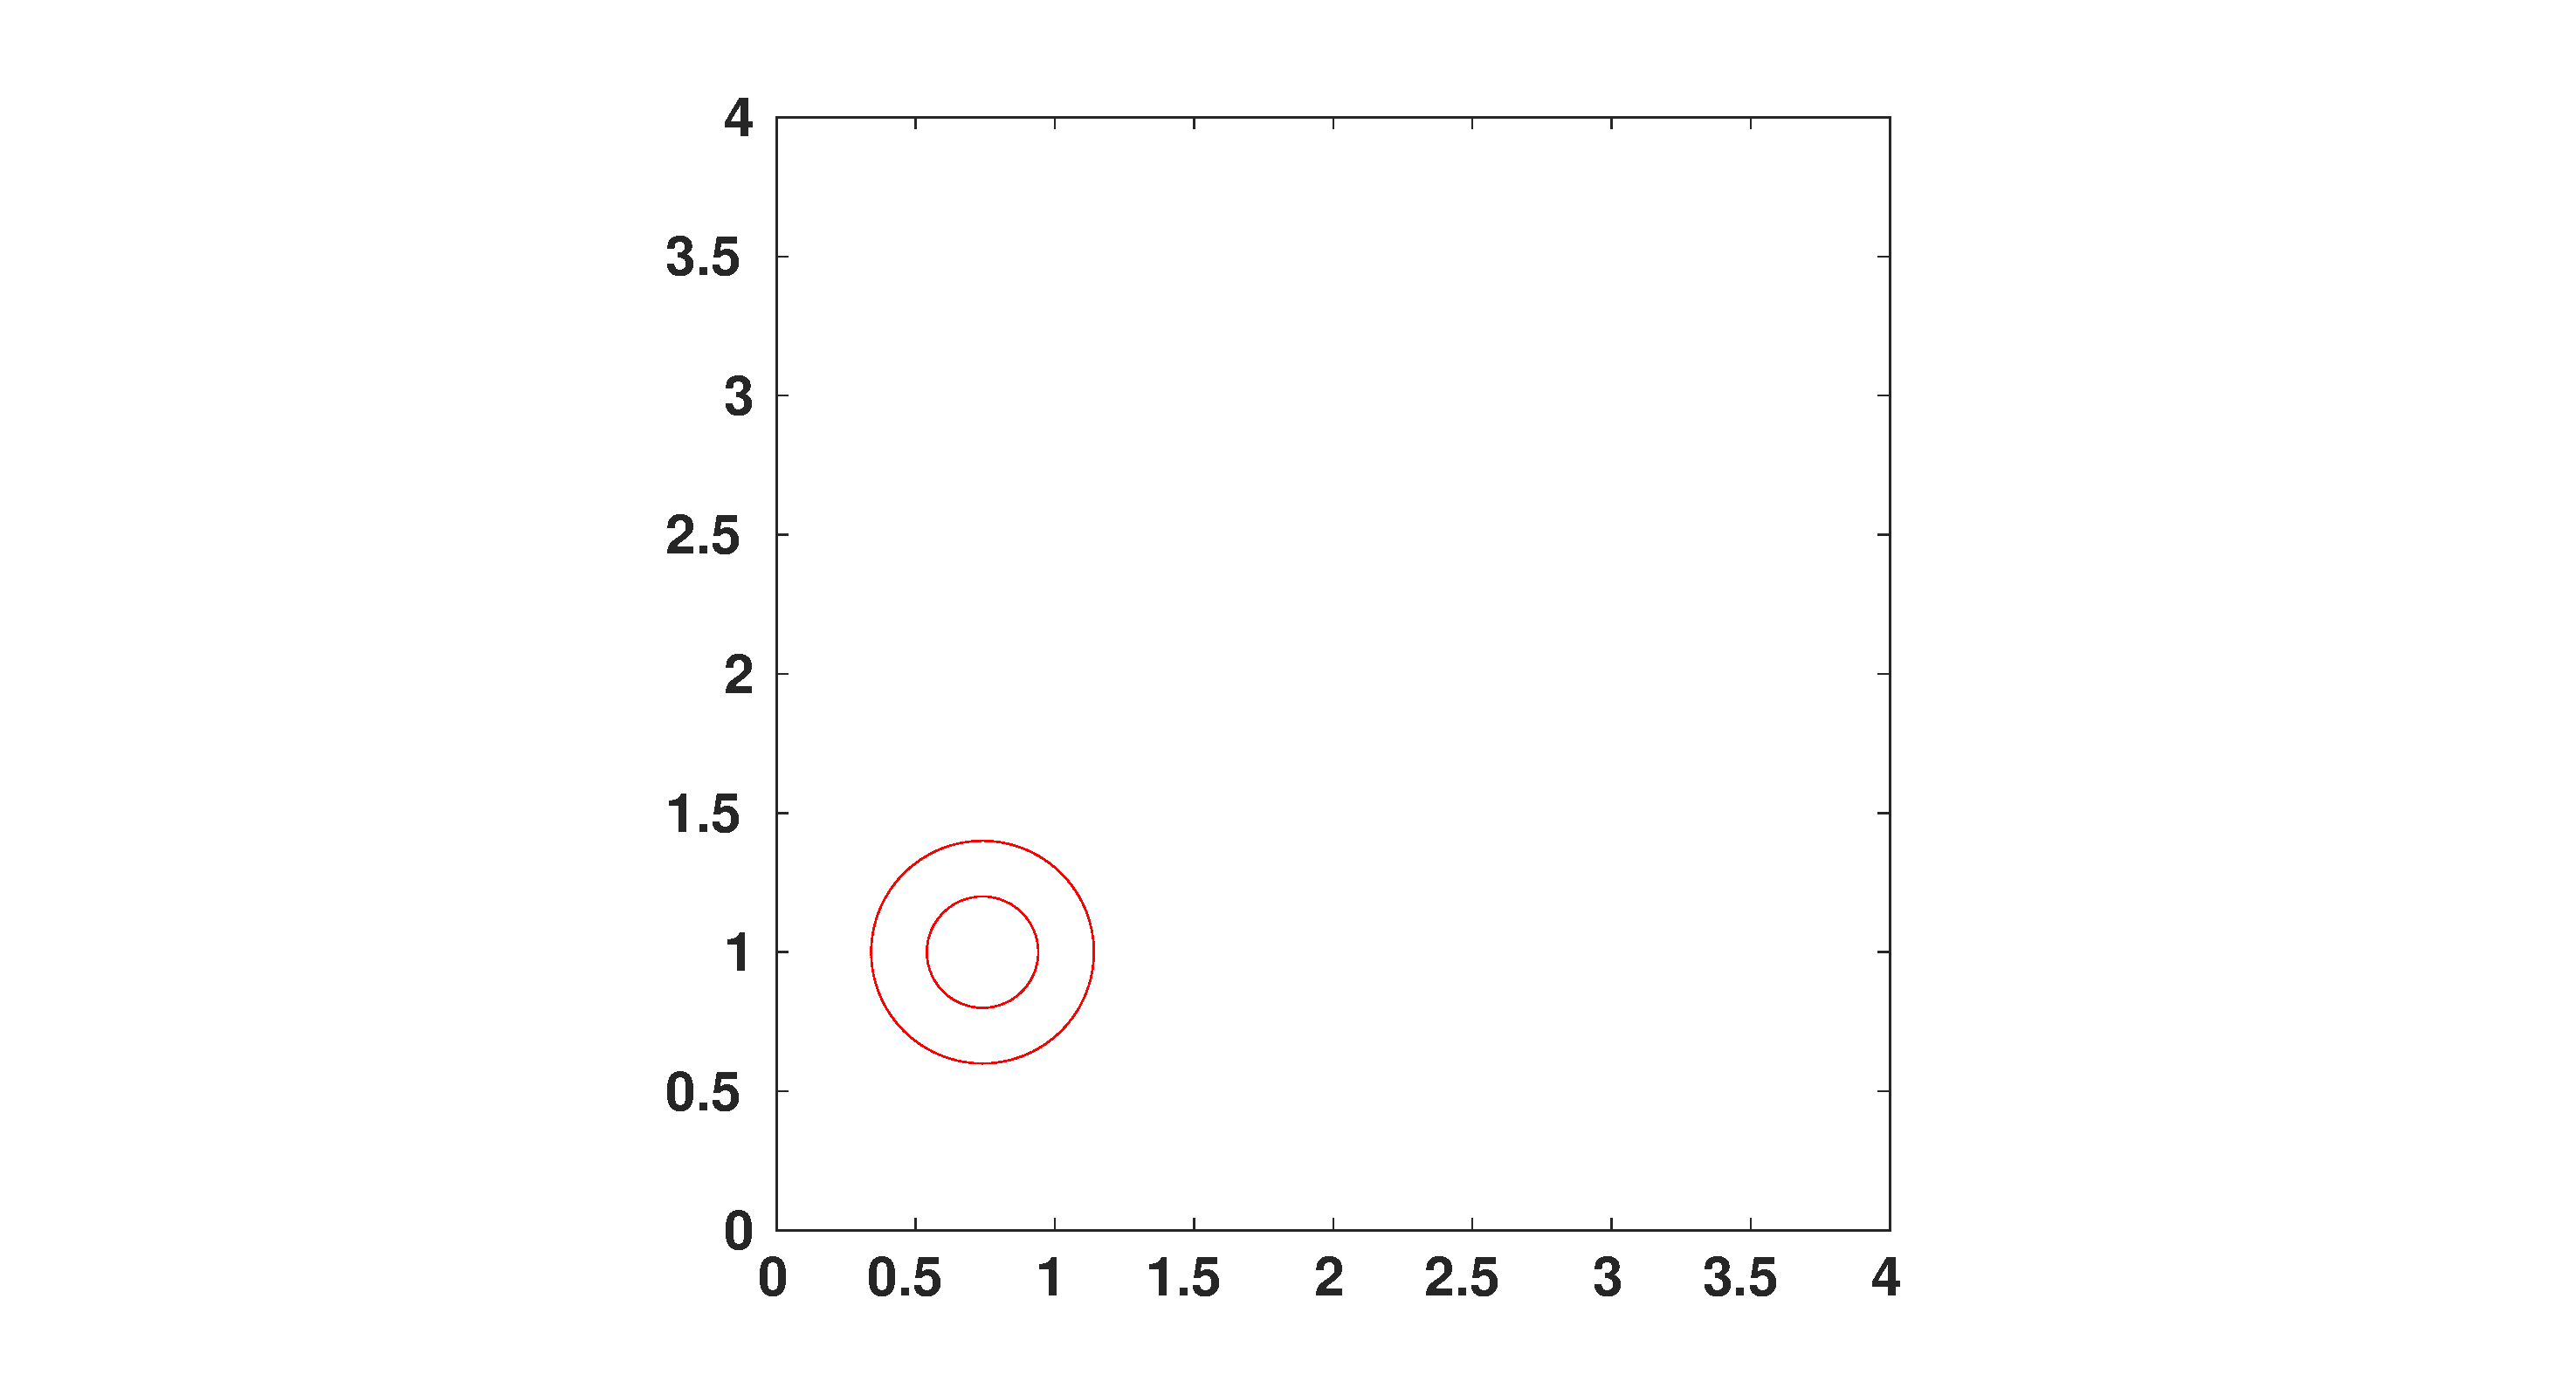
\includegraphics[width=0.5\textwidth]{CD_0.eps}
      }
   \subfloat[After advecting Volume Fraction for 20 time steps ]{%
      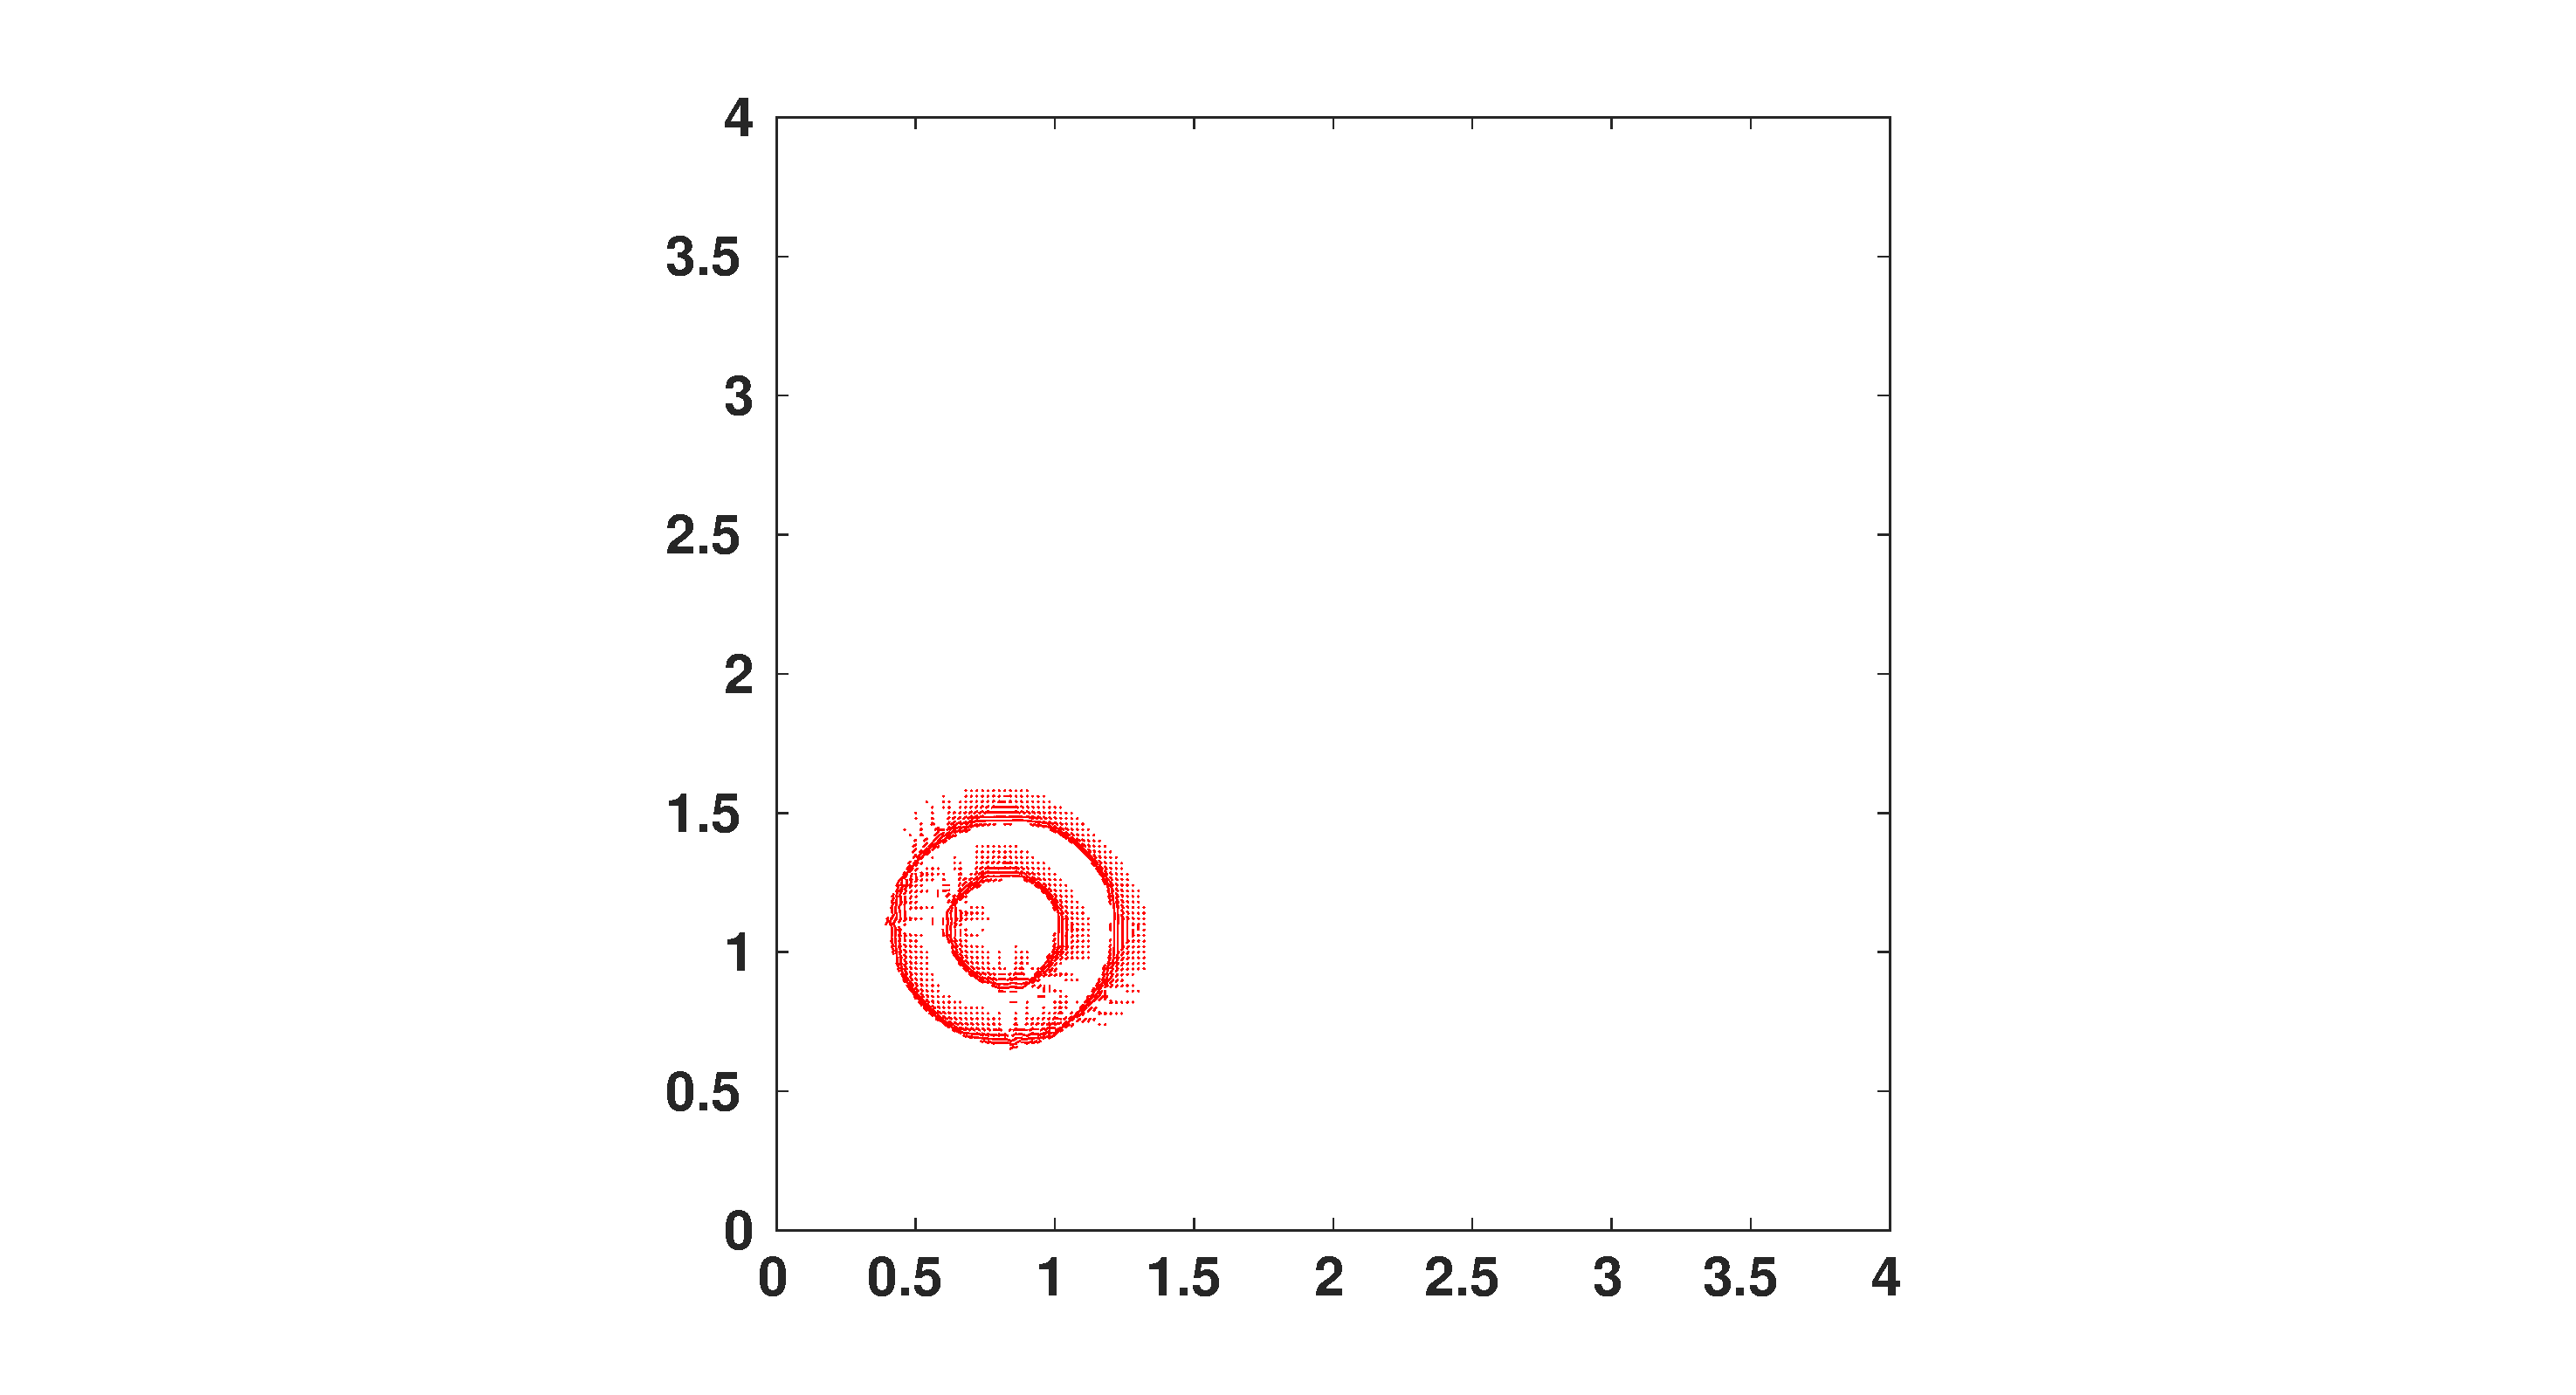
\includegraphics[width=0.5\textwidth]{CD_20.eps}
      } \\
        \subfloat[After Volume Fraction density for 20 time steps ]{%
      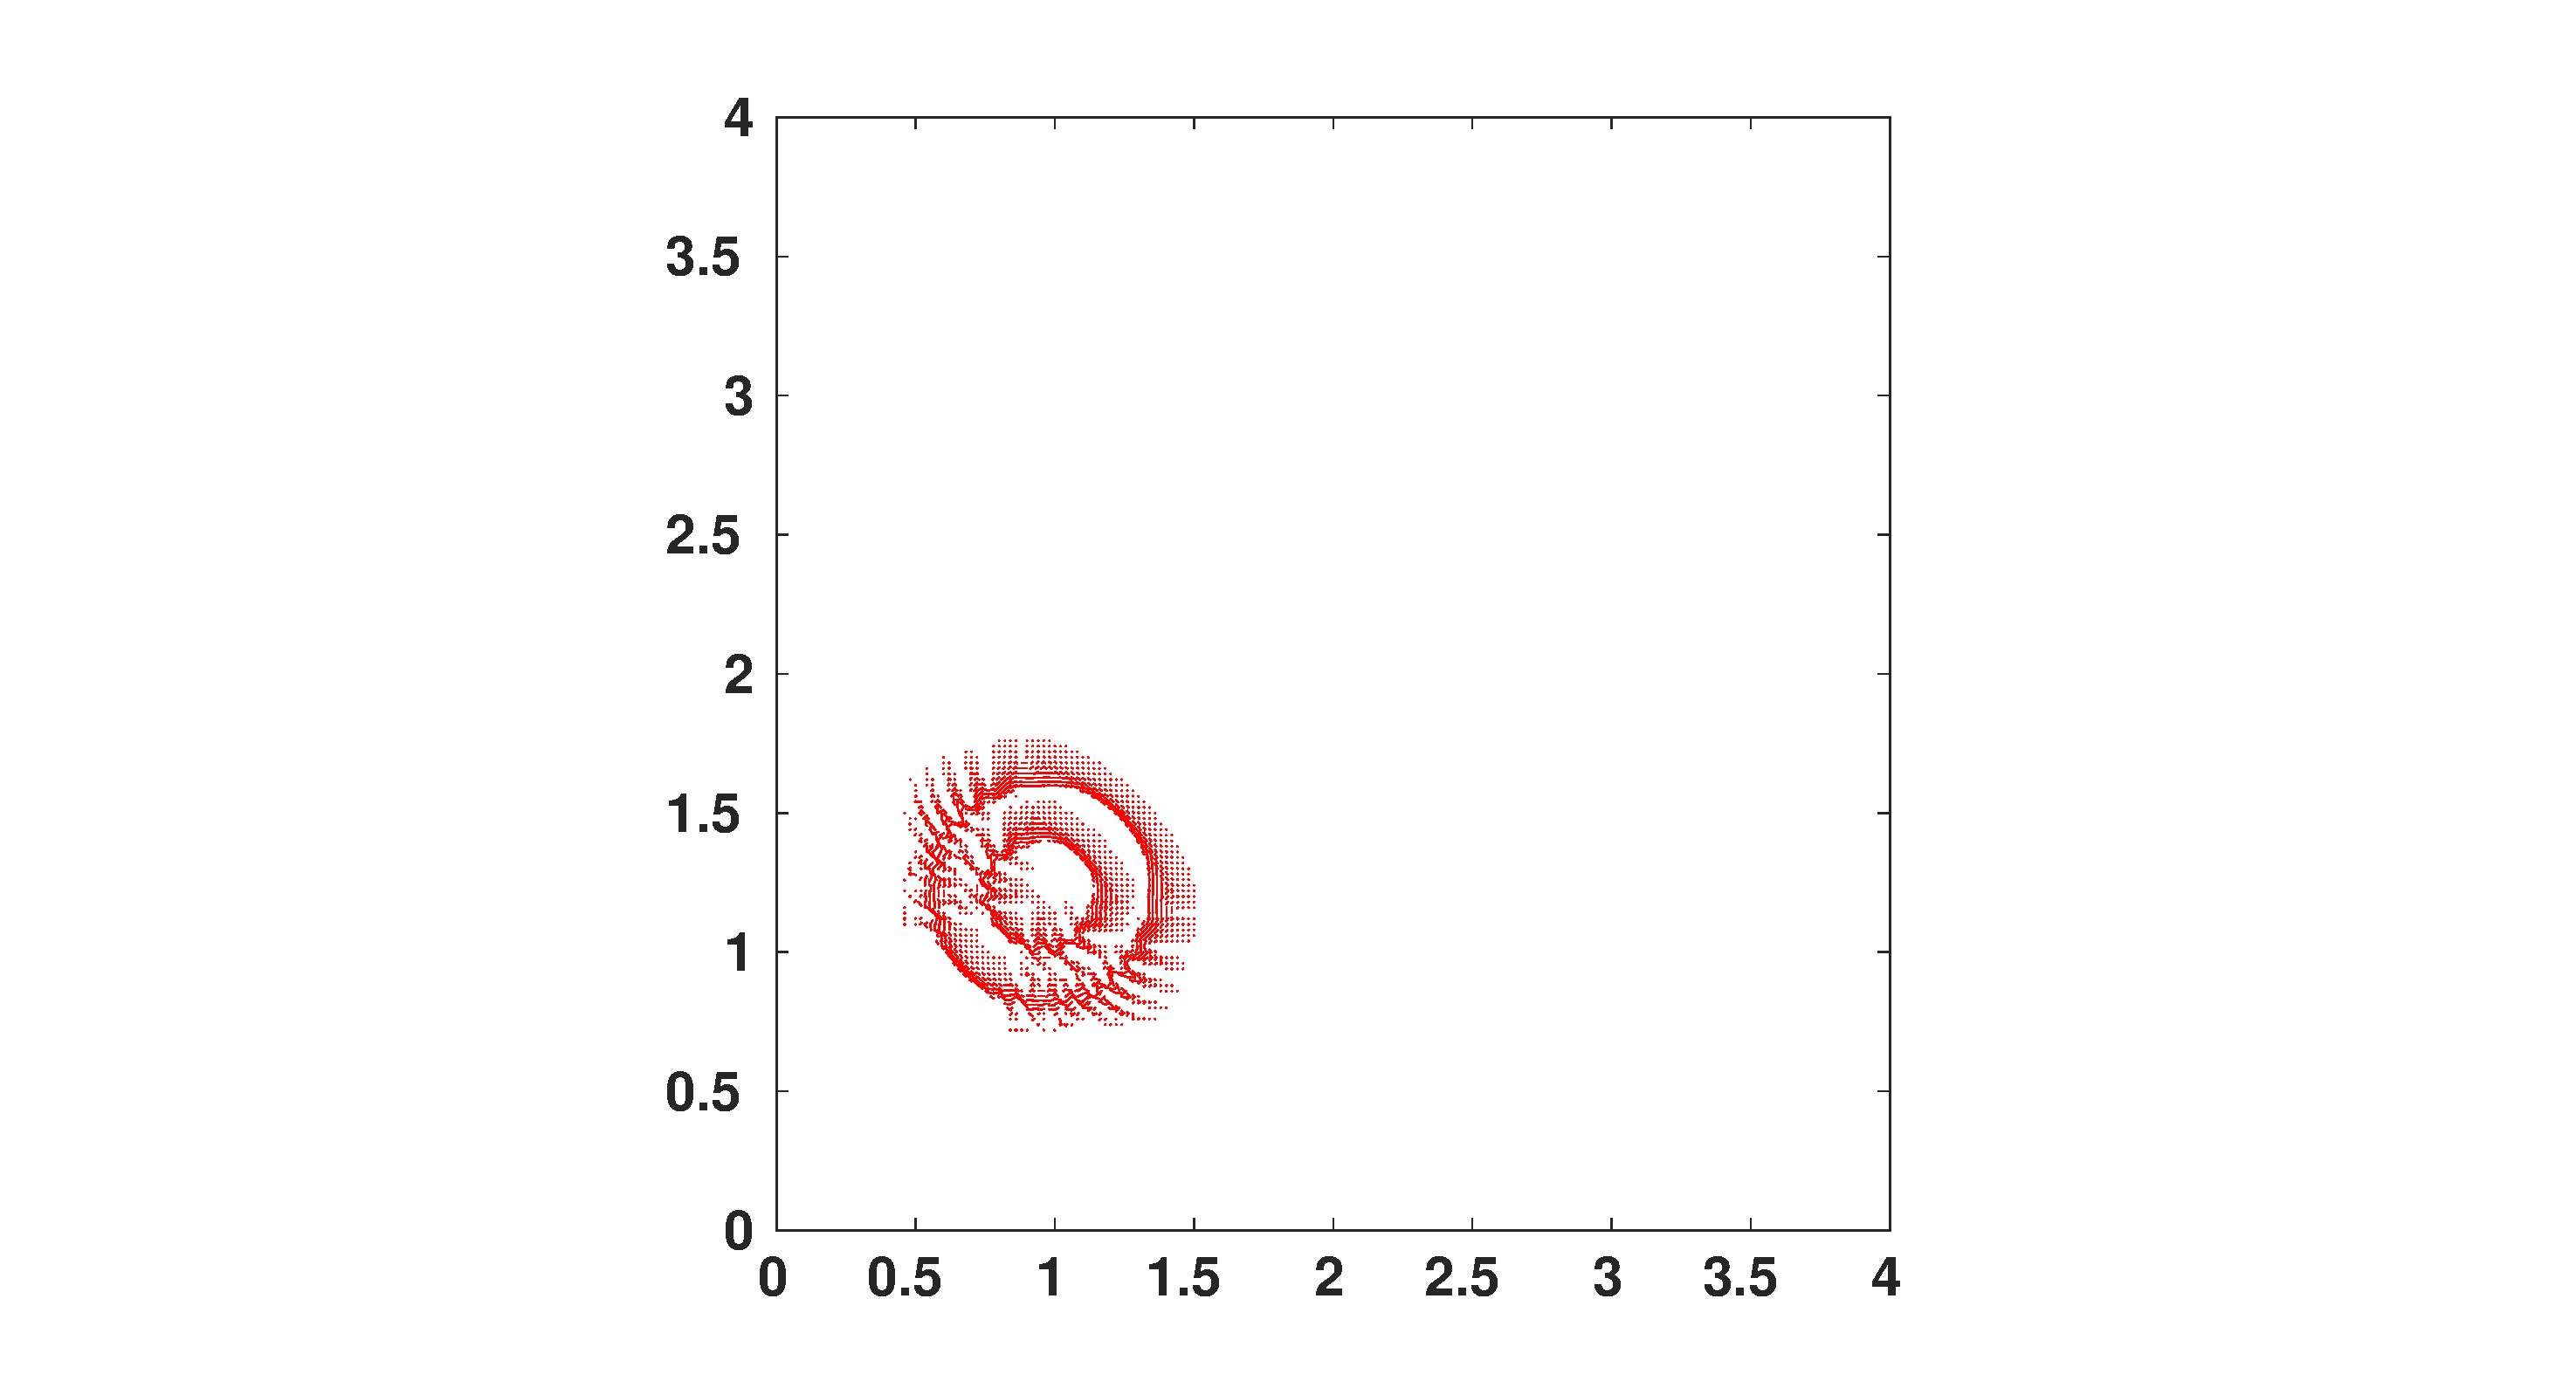
\includegraphics[width=0.5\textwidth]{CD_50.eps}
      }
        \subfloat[After Volume Fraction density for 50 time steps ]{%
      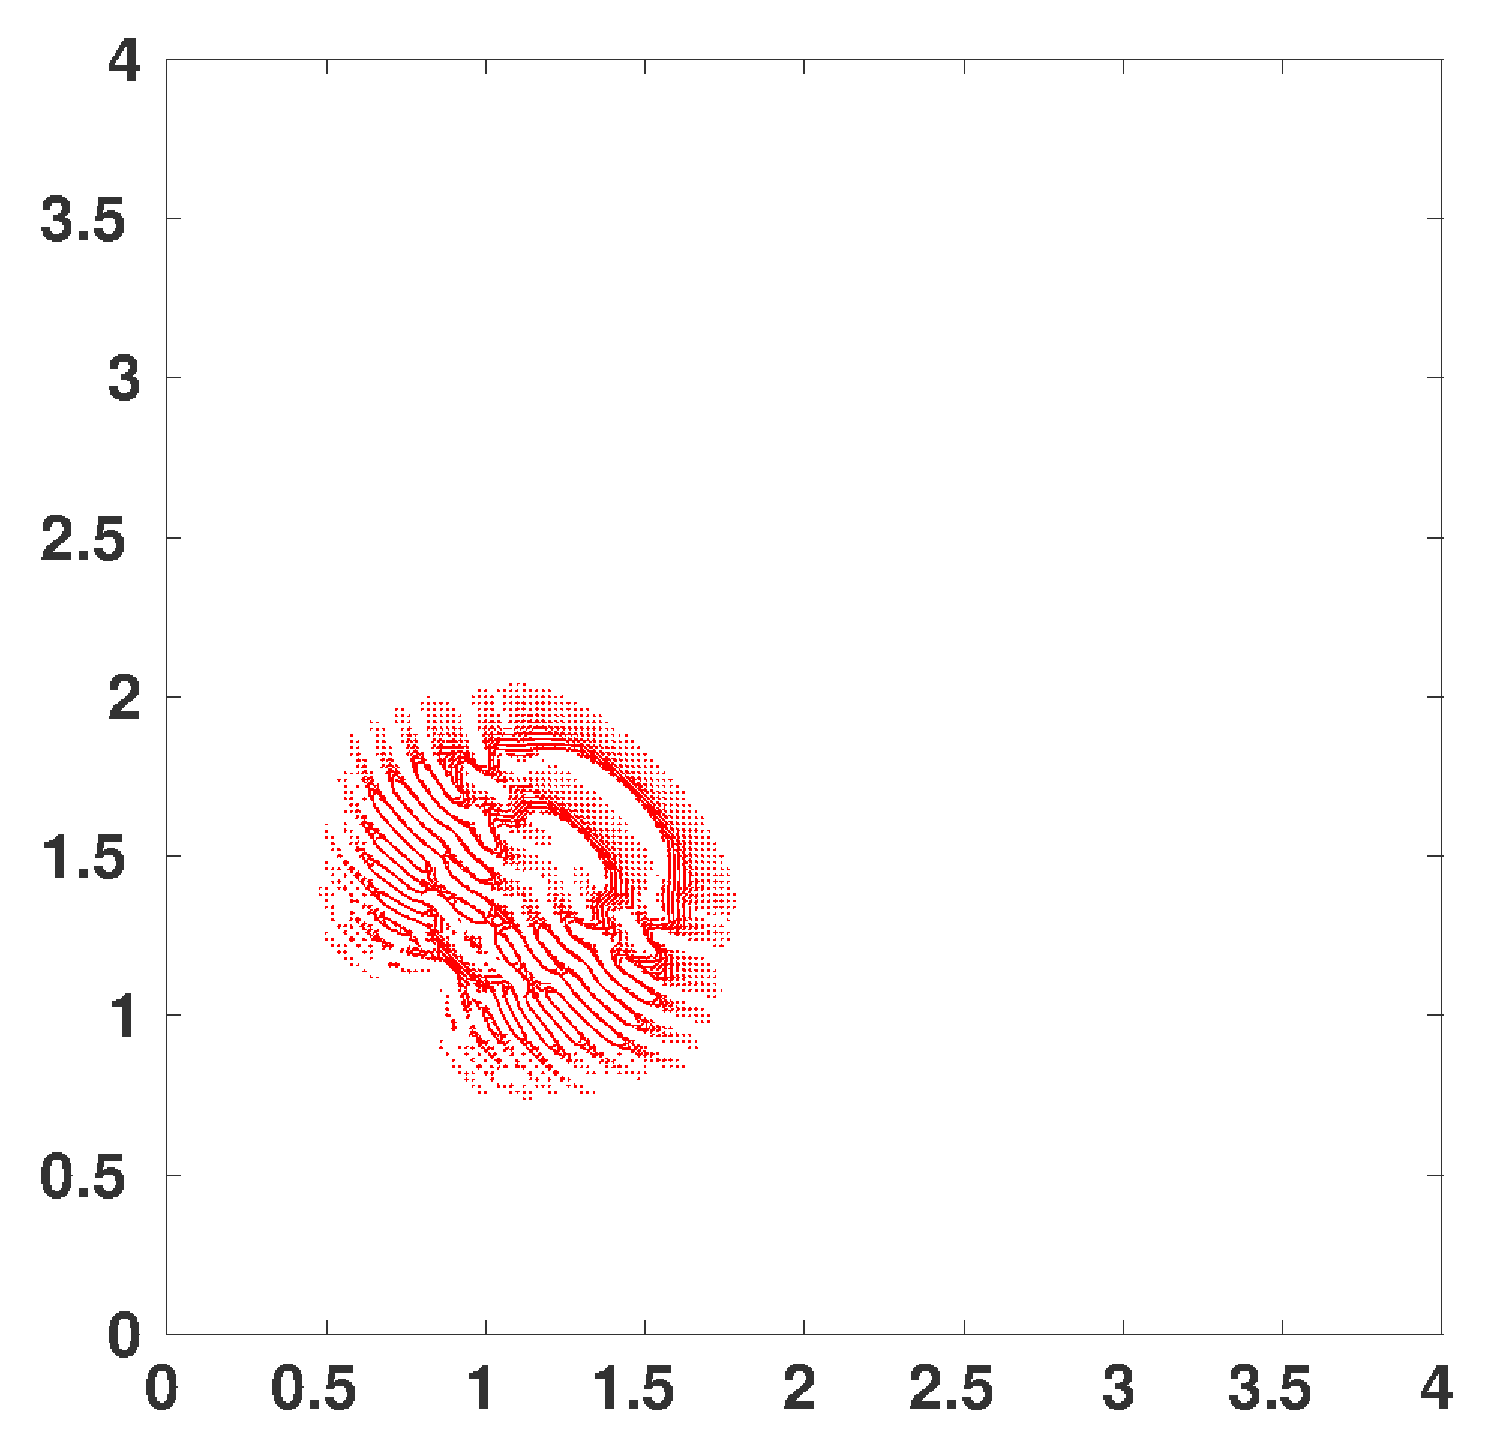
\includegraphics[width=0.5\textwidth]{CD_100.eps}
      }
 \caption{Advection of Volume Fraction using finite difference method}
 \label{Fig:smearing}
\end{figure}

\subsection{Interface Reconstruction}
As interface in Volume of fluid method can be reconstructed in many ways we choose the Least Squares Volume of 
Fluid Reconstruction Algorithm proposed by \cite{Pilliod2004} which is one of the most accurate algorithm available in literature. It is second order accurate in space 
and can be extended to the 3D. It represents the interface as a line in 2D and a plane in 3D. The VOF method achieves higher accuracy using geometrical techniques to reconstruct
and advect the interface.
Any interface reconstruction algorithm consists two basic steps:-
\begin{enumerate}
 \item Interface Reconstruction
 \item Advection of F field
\end{enumerate}
There are many steps involved in interface reconstruction explained and these are in following subsections.{\vspace{3cm}}\\
\underline{Least Squares of Volume of Fluid Interface Reconstruction Algorithm}
\subsubsection{Step I : Obtain F field}
At first an F-field is obtained by knowing the initial free surface and then by calculating the F values for each cell. 
For reconstruction of interface a cell having a value of F between 0 and 1 is located.

\subsubsection{Step II : Initial guess of slope}
The initial slope of the normal to the interface away from the dark fluid can obtained using (Green-Gauss gradient \cite{Gerlach2006}) which is  given by 
\begin{eqnarray}
  N_x=-\frac{1}{\Delta x}{[F_{r+1,c+1}+2F_{r,c+1}+F_{r-1,c+1}-F_{r+1,c-1}-2F_{r,c-1}-F_{r-1,c-1}]} \\
  N_y=-\frac{1}{\Delta y}{[F_{r+1,c+1}+2F_{r+1,c}+F_{r+1,c-1}-F_{r-1,c+1}-2F_{r-1,c}-F_{r-1,c-1}]}
  \label{Eq:GG}
\end{eqnarray}

\subsubsection{Step III: Quadrant Identification}
To get the interface as a line in 2D, we have to determine its shape and orientation in a cell. First step is to get the normal orientation in the quadrant.
 Signs of $N_x$ and $N_y$ will determine the quadrant in which the normal points away from the dark fluid present in the cell. 
  \begin{figure}%[H]
  \centering
   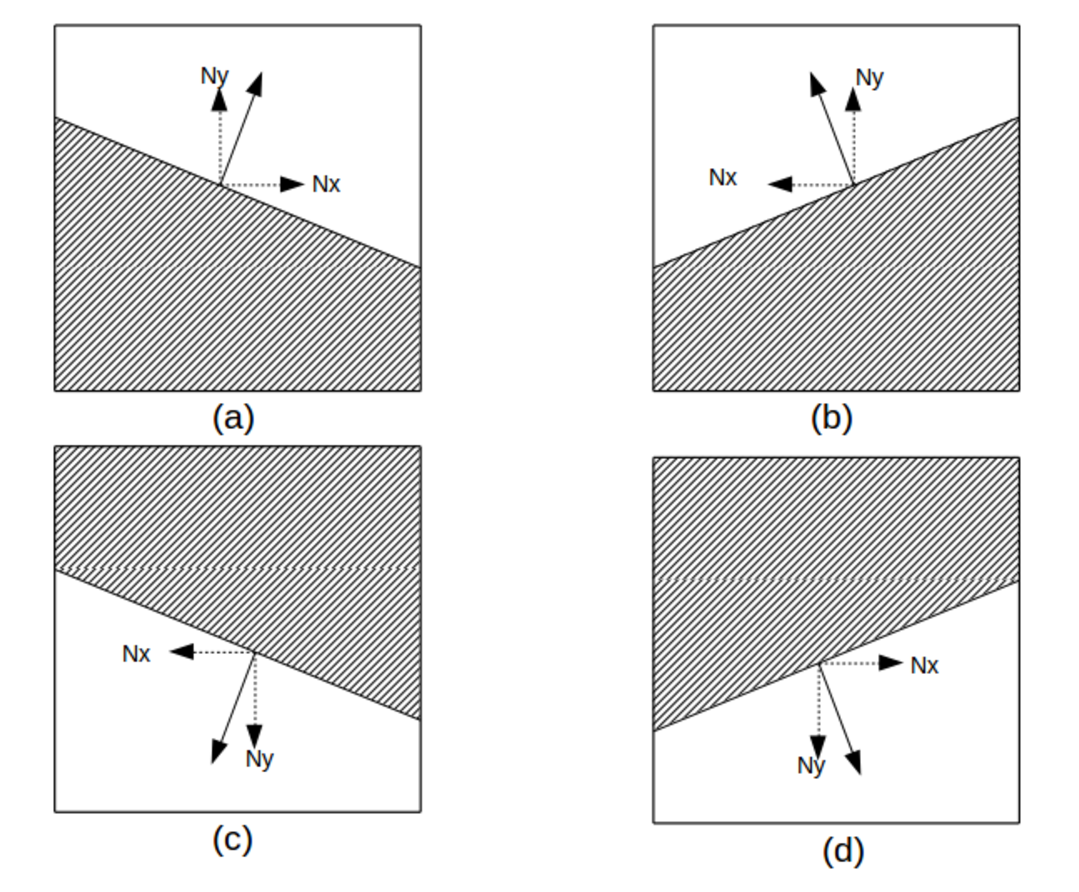
\includegraphics[scale=0.4]{quad.eps}
   \caption[Interface normal direction]{(a)I Quad (b) II Quad (c) III Quad (d) IV Quad }
   \label{Fig:quad}
  \end{figure}

\subsubsection{Step IV: Angle Calculation}
 The angle, $\theta$ is the positive acute angle made by the interface with x-axis if the normal points into first and the third quadrant and positive acute angle made by 
 the interface by y-axis if the normal points into the second and fourth quadrant. This definition is necessary because we treat all other quadrants as the $I^{st}$ quadrant
 by suitable rotation. So for the second and the fourth quadrant $\theta$ has to be redefined. Refer to Figure \ref{Fig:quad} for definition of theta. This is 
 required to do since the algorithm is developed in way it works for normal in first quadrant and all other cases has to be modified according to algorithm.
% 
%  Equation \ref{Eq:angle} gives the expression for calculating $\theta$
% \begin{equation}
%  \theta=\frac{\pi}{2}-tan^{-1}\left(\frac{N_x}{N_y}\right)
%  \label{Eq:angle}
%  \end{equation}
% \begin{wrapfigure}{r}{0.5\textwidth}
%   \begin{center}
%     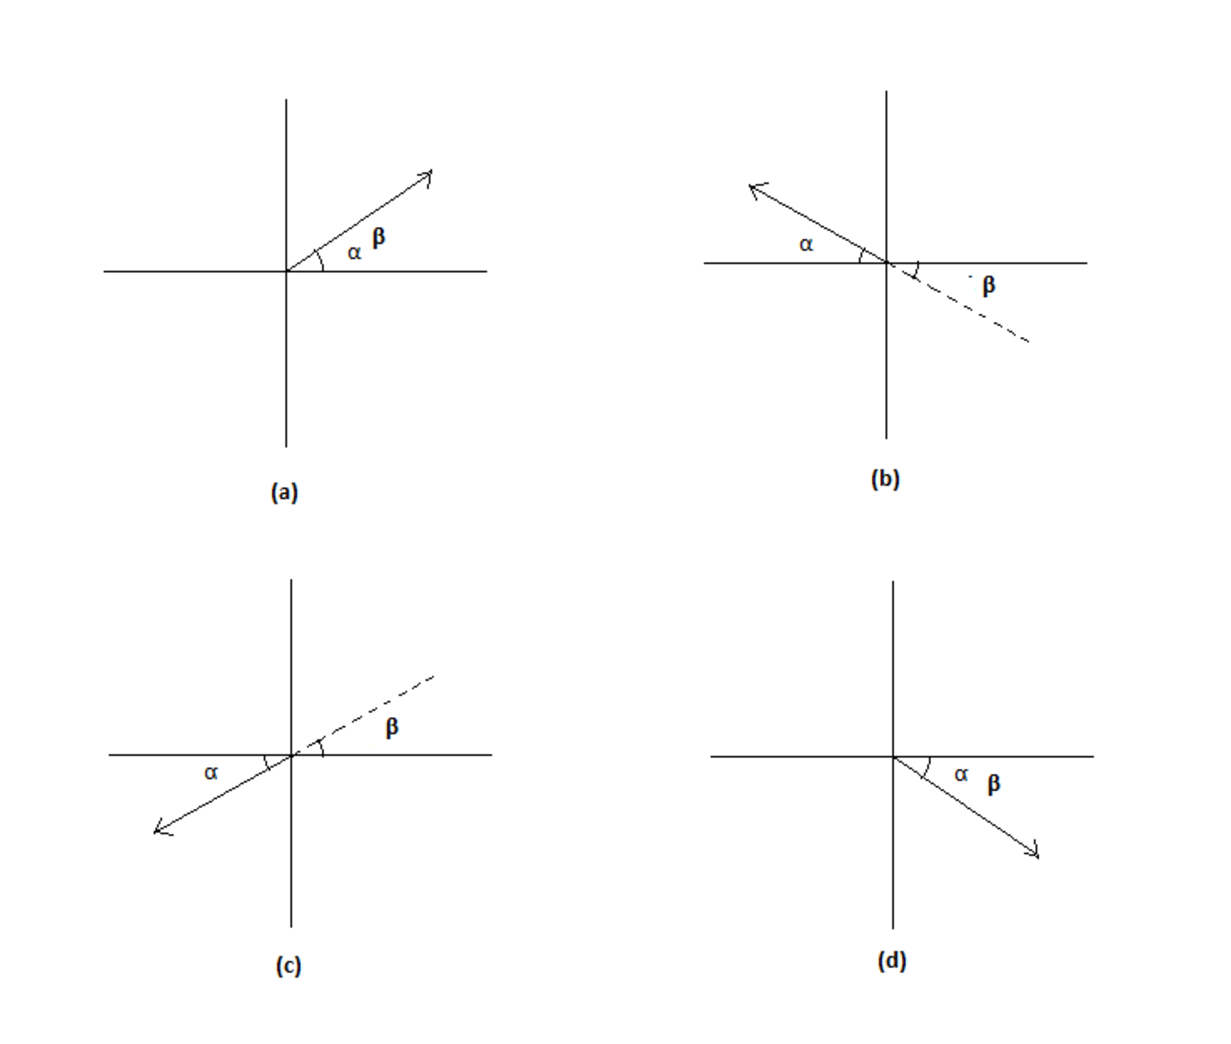
\includegraphics[width=0.48\textwidth]{atan.eps}
%   \end{center}
%   \caption{Angle value returned by gcc compiler}
%     \label{Fig:gcc}
% \end{wrapfigure}
%  
% The function atan() in GCC returns a value between $\frac{-\pi}{2}$ and $\frac{\pi}{2}$ as shown in Figure \ref{Fig:gcc}. The slope, $\frac{N_y}{N_x}$ of normal to interface
% is given as input to atan$\left(\frac{N_y}{N_x}\right)$ return the value of the acute angle made by the x-axis. 
% The returned value is positive when in first and third quadrant and negative when in second and fourth quadrant. 
% To make it positive the fabs function is used.
% \begin{eqnarray*}
% \beta = atan\left(\frac{N_y}{N_x}\right), 
% \qquad \alpha =\lvert\beta\lvert 
% \end{eqnarray*}
% 
% Hence, the expression for GCC to calculate theta becomes
% 
\begin{equation}
 \theta=\frac{\pi}{2}-fabs\left(atan\left(\frac{N_x}{N_y}\right)\right)
 \end{equation}
%  Note: Every step after calculating $\theta$, will have first reorient the normal to the first quadrant.
% The code treats all the quadrants as the first quadrant after suitable rotation.
 
\subsubsection{Step V: Shape Identification}
There are four possible shapes in a 2D reconstruction 
If the volume fraction and $\theta$ is fixed then the shape is decided as in Figure \ref{Fig:shape_region}. The various regions are identified as follows.
\begin{figure}
 \centering
    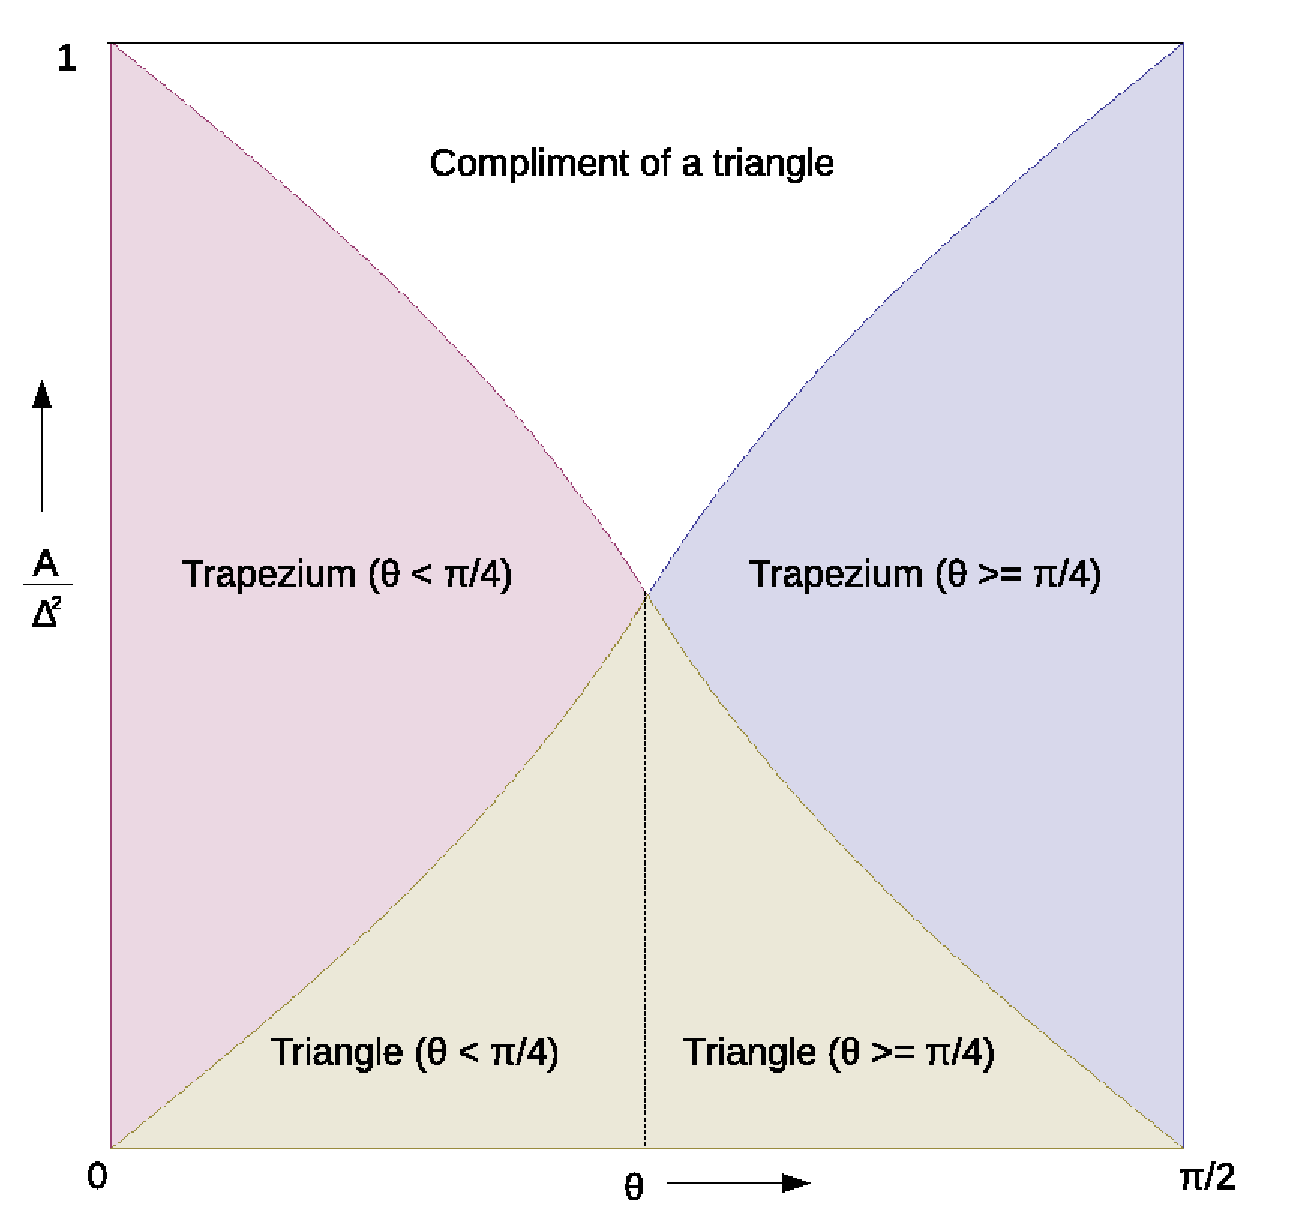
\includegraphics[scale=0.5]{shape_region.eps}
  \caption{Area and angle region}
  \label{Fig:shape_region}
\end{figure}
\underline{Triangle}\\
Area of fluid, $A=\Delta^2F$ 

From Figure \ref{Fig:triangle}, we get,

\begin{figure}%[H] 
\centering
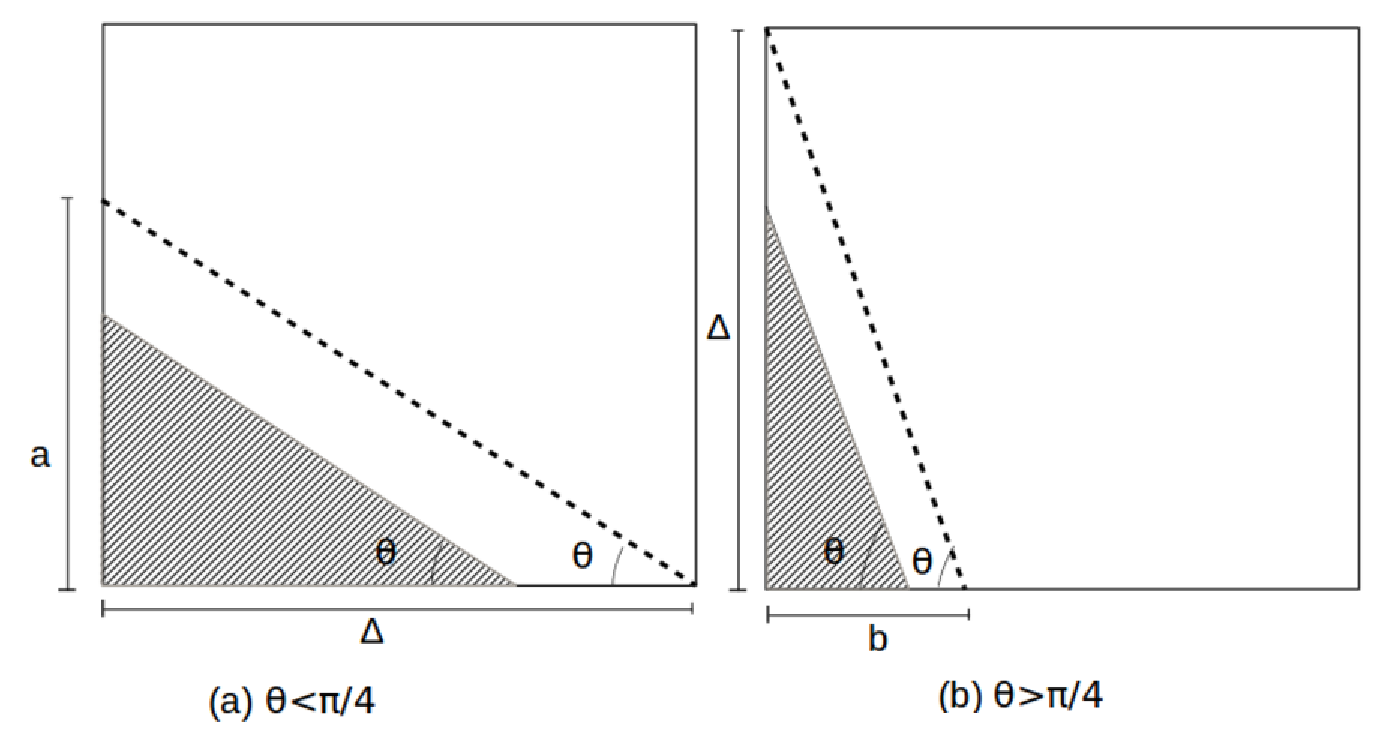
\includegraphics[scale=0.4]{triangle.eps}
\caption{Area of the triangle made by dark fluid in the cell}
\label{Fig:triangle}
\end{figure}

\begin{eqnarray*}
 a&=&\Delta tan\theta \text{\quad $\theta < \frac{\pi}{4}$} \\  
 b&=&\frac{\Delta}{tan\theta} \text{\quad $\theta >= \frac{\pi}{4}$}\\
\end{eqnarray*}

\begin{equation*}
\boxed{\begin{align}
    \frac{A}{\Delta^2} <= \frac{1}{2} tan\theta \qquad \text{for, }\theta < \frac{\pi}{4} \\
    \frac{A}{\Delta^2}<=  \frac{1}{2tan\theta} \qquad \text{for, }\theta > \frac{\pi}{4}   
    \end{align}}
\end{equation*}

\underline{}{For trapezium},\\

\begin{figure}%[H]
\centering
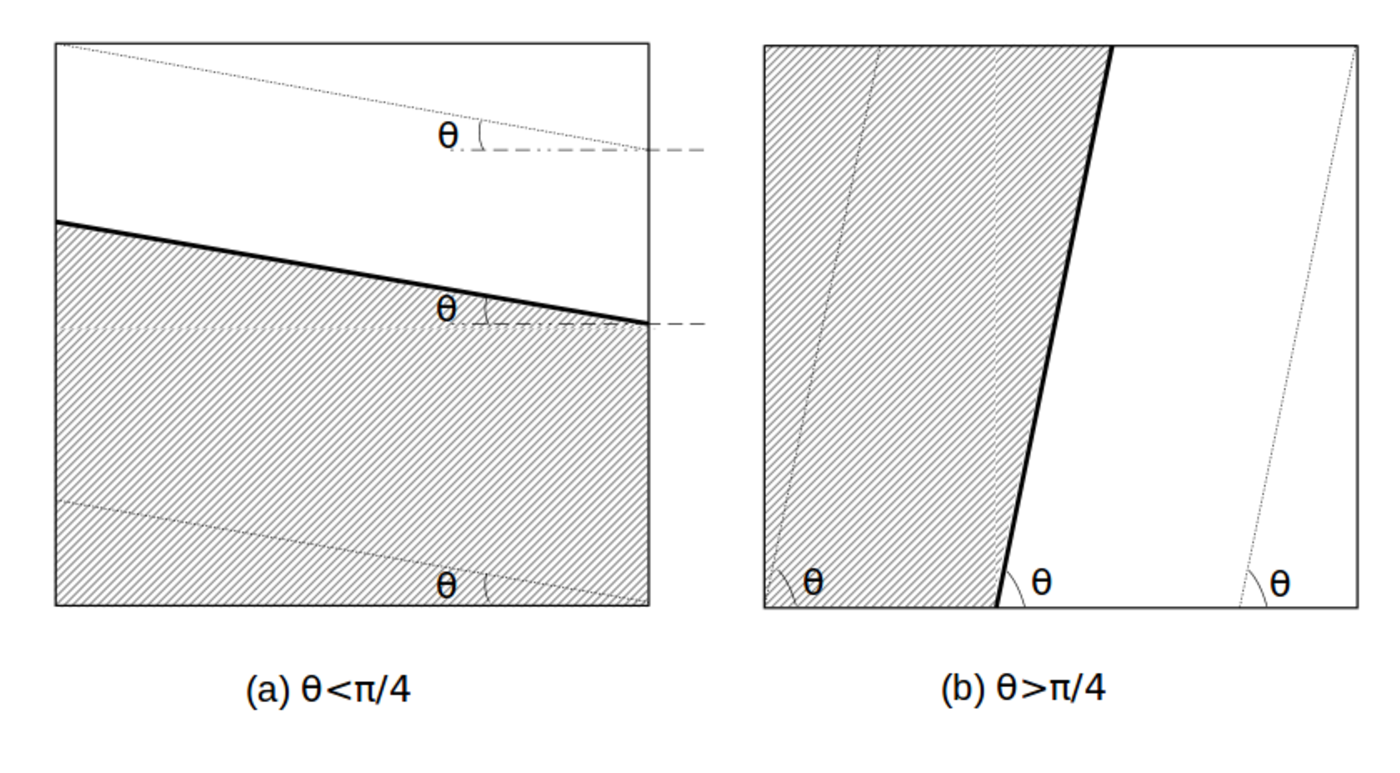
\includegraphics[scale=0.4]{trapezium.eps}
\caption{Area of a trapezium made by the dark fluid in the cell}
\end{figure}

\begin{figure}
 \centering
 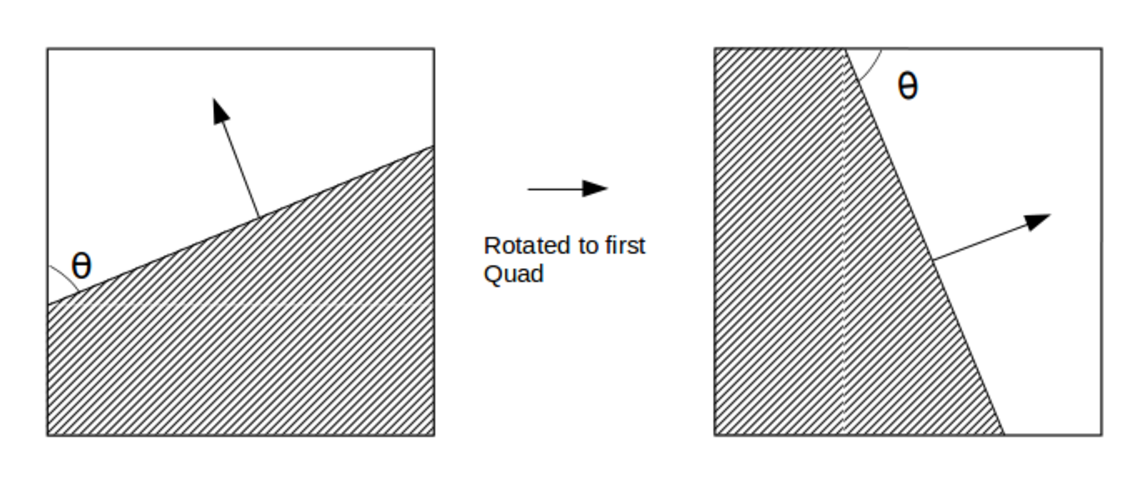
\includegraphics[scale=0.6]{2ndQuad.eps}
 \caption{When the cell is reoriented to make normal lie in first quadrant}
 \label{Fig:reorientation}
\end{figure}

In Figure \ref{Fig:reorientation}, it can be seen that when the cell reoriented to make the normal in first quadrant the $\theta$ becomes the angle with the horizontal axis.
Hence, the same calculations can be applied to this cell for what is done for first quadrant. 

\begin{equation*}
\boxed { \begin{align}
 \frac{1}{2} tan\theta <& \frac{A}{\Delta^2}< \left(1-\frac{1}{2} tan\theta\right)  \qquad \text{for, } \theta < \frac{\pi}{4} \nonumber	\\    
   \frac{1}{2tan\theta} <&   \frac{A}{\Delta^2}< \left(1-\frac{1}{2tan\theta}\right) \qquad \text{for, }  \theta >= \frac{\pi}{4}	
   \end{align}}
\end{equation*}
For all other cases the shape becomes a compliment of a triangle.

\subsubsection{Step VI: Perpendicular distance Calculation }
After reorientation, the perpendicular distance will now be always from the LHS corner of the cell.\\
\underline{Triangle}\\
Note the following formulae for Figure \ref{Fig:trianlge_p}

\begin{eqnarray*}
c=\frac{b}{cos\theta},
\qquad b=\frac{p}{sin\theta},  
\qquad  c=\frac{p}{sin\theta cos\theta},
\qquad   \frac{1}{2}pc=F\Delta^2,
\qquad  \frac{p^2}{sin2\theta}=F\Delta^2 \nonumber
\end{eqnarray*}

\begin{equation*}
\boxed{ \begin{align}
  p=\sqrt{F\Delta^2sin2\theta}
  \end{align} }
\end{equation*}
  
\begin{figure}
\centering
 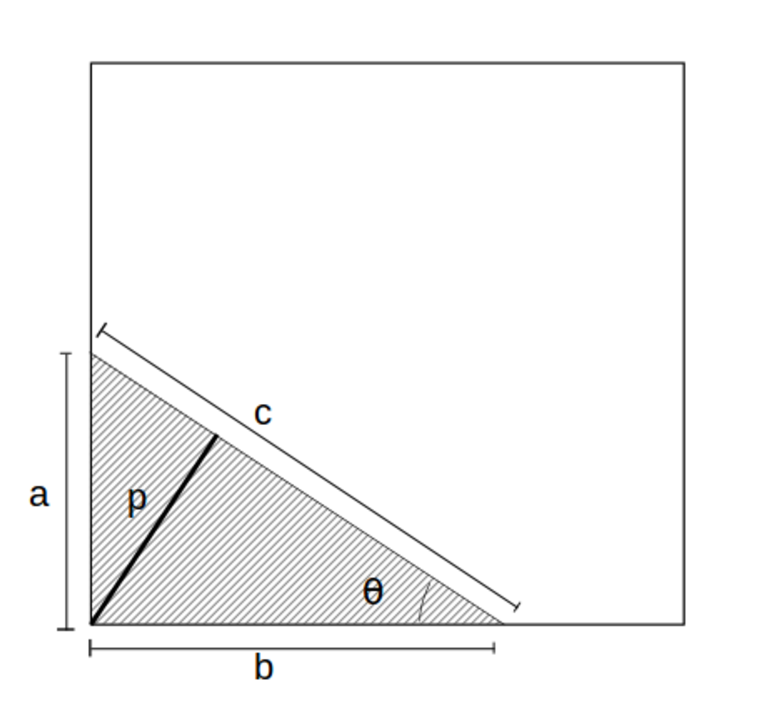
\includegraphics[scale=0.4]{triangle_p.eps}
 \caption{Perpendicular distance in a triangle}
 \label{Fig:trianlge_p}
\end{figure}

\underline{Trapezium}, \\
  \begin{figure}
  \centering
    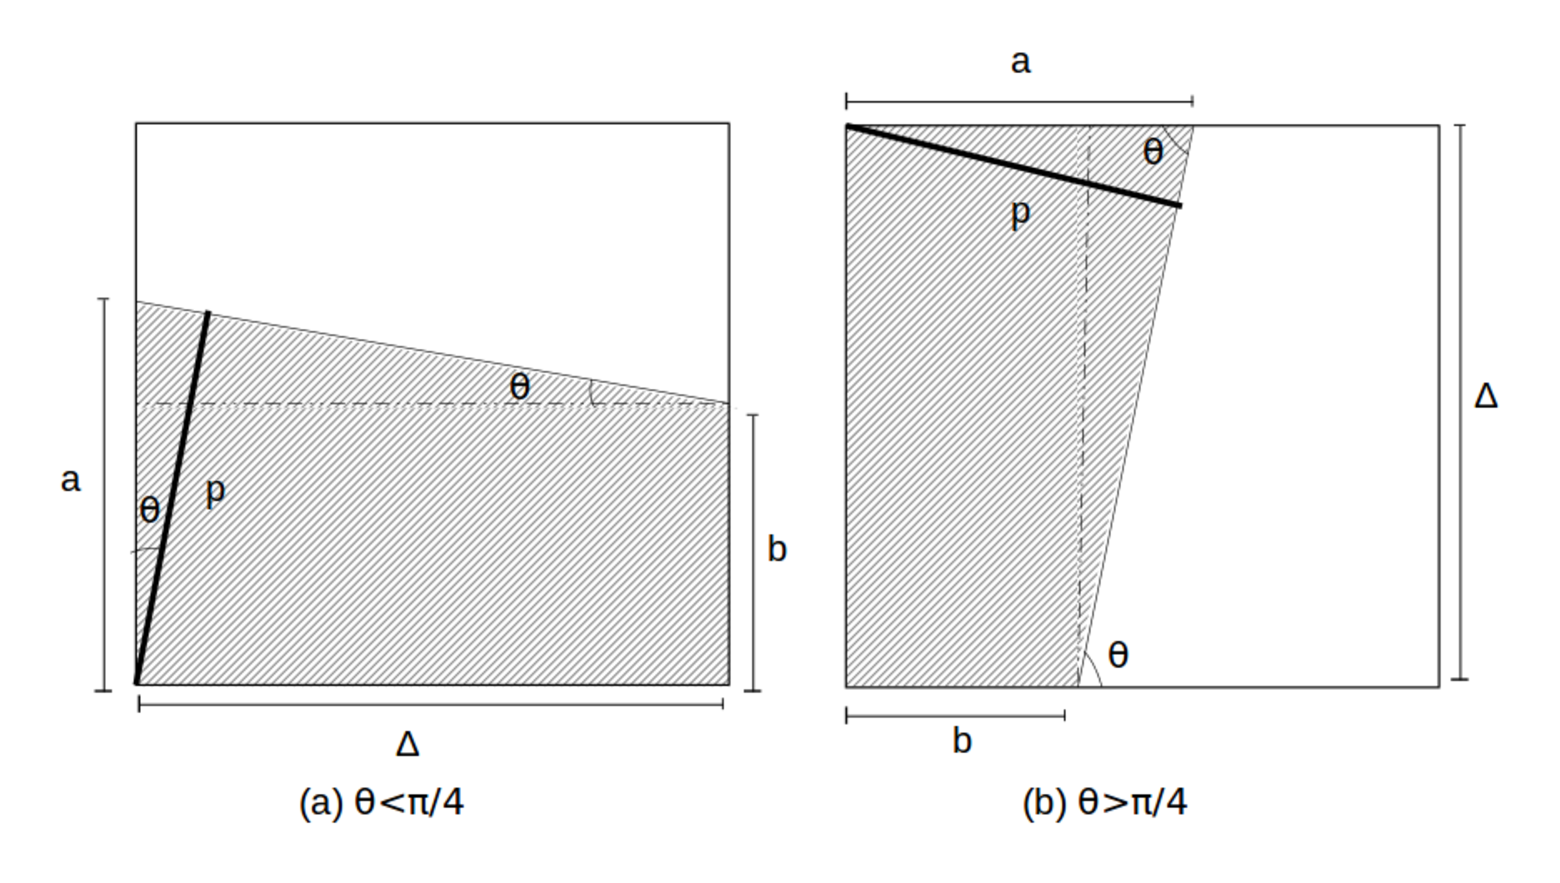
\includegraphics[scale=0.4]{trapezium_p.eps}
    \caption{Perpendicular distance for a trapezium}
    \label{Fig:trapezium_p}
  \end{figure}
  Note the formulae for Figure \ref{Fig:trapezium_p}
  
  \begin{equation*}
  \begin{aligned}  
     \text{For} \quad \theta  < \frac{\pi}{4}, 
    \qquad  \Delta^2 F &=\frac{(a+b)\Delta}{2},
    \qquad a=\frac{p}{cos\theta},
      \qquad tan\theta=\frac{a-b}{\Delta},
      \qquad b=\frac{p}{cos\theta}-\Delta tan\theta, \\
      \\
      \text{or,}\qquad \frac{1}{2}\Delta\left(\frac{2p}{cos\theta}-\Delta tan\theta\right)&=\Delta^2 F,
      \qquad \boxed{p=\Delta Fcos\theta+\frac{1}{2}\Delta sin\theta} \\
      \\
\text{For} \quad \theta  >= \frac{\pi}{4},
\qquad
\Delta^2 F &=\frac{(a+b)\Delta}{2}
\qquad
a=\frac{p}{sin\theta},
\qquad
tan\theta=\frac{\Delta}{a-b},
\qquad
b=\frac{p}{sin\theta}-\frac{\Delta}{tan\theta},\\
\\
\text{or,}\qquad 0.5\Delta\left(\frac{2p}{sin\theta}-\frac{\Delta}{tan\theta}\right)&=\Delta^2 F,
\qquad
\boxed{p=\Delta Fsin\theta+\frac{1}{2}\Delta cos\theta}
\end{aligned}
  \end{equation*}
  
\underline{For compliment of triangle},
\begin{figure}[H]
\centering
 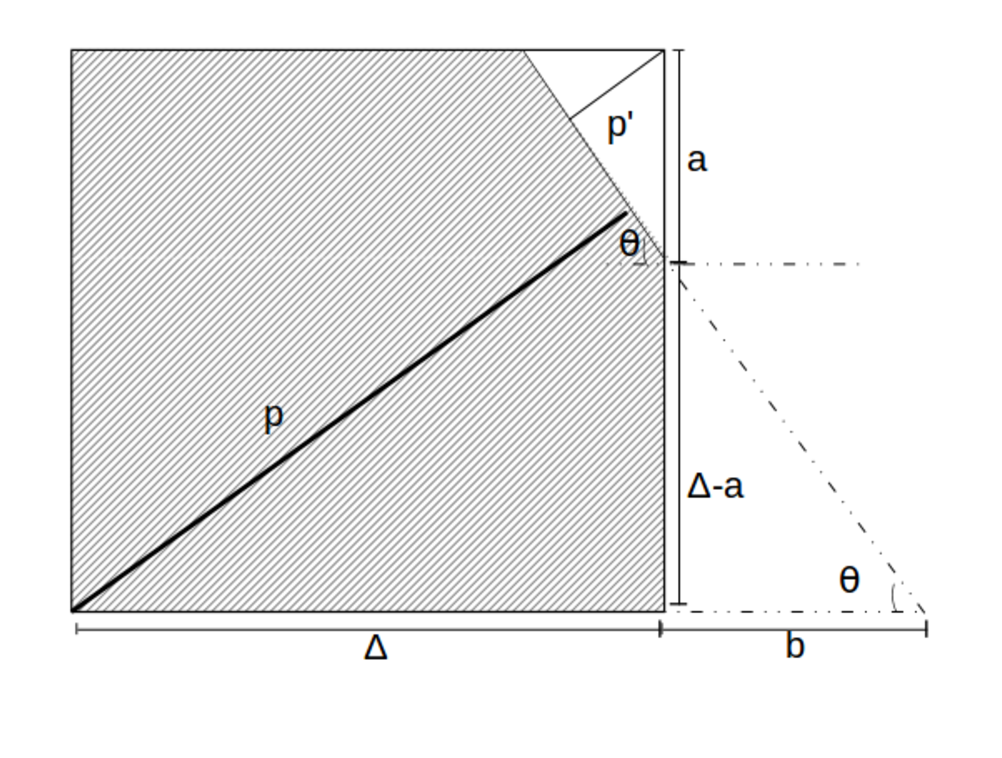
\includegraphics[scale=0.3]{compliment_p.eps}
 \caption{Perpendicular distance for compliment of the triangle}
\end{figure}

\begin{equation*}
\begin{align}
 p'&=&\sqrt{F\Delta^2sin2\theta},
\qquad a=\frac{p'}{cos\theta},\\
\\
\text{or,}\qquad b&=&\frac{\Delta-a}{tan\theta},
\qquad \boxed{p=\Delta(sin\theta+cos\theta)-p'}
\end{align}
\end{equation*}

\subsubsection{Step VII : Line Extrapolation}
After, reorientation of the line to the first quadrant. A line can be constructed with the $\theta$ and perpendicular distance using normal form, (See Figure \ref{Fig:normal})
\begin{figure}
 \centering
 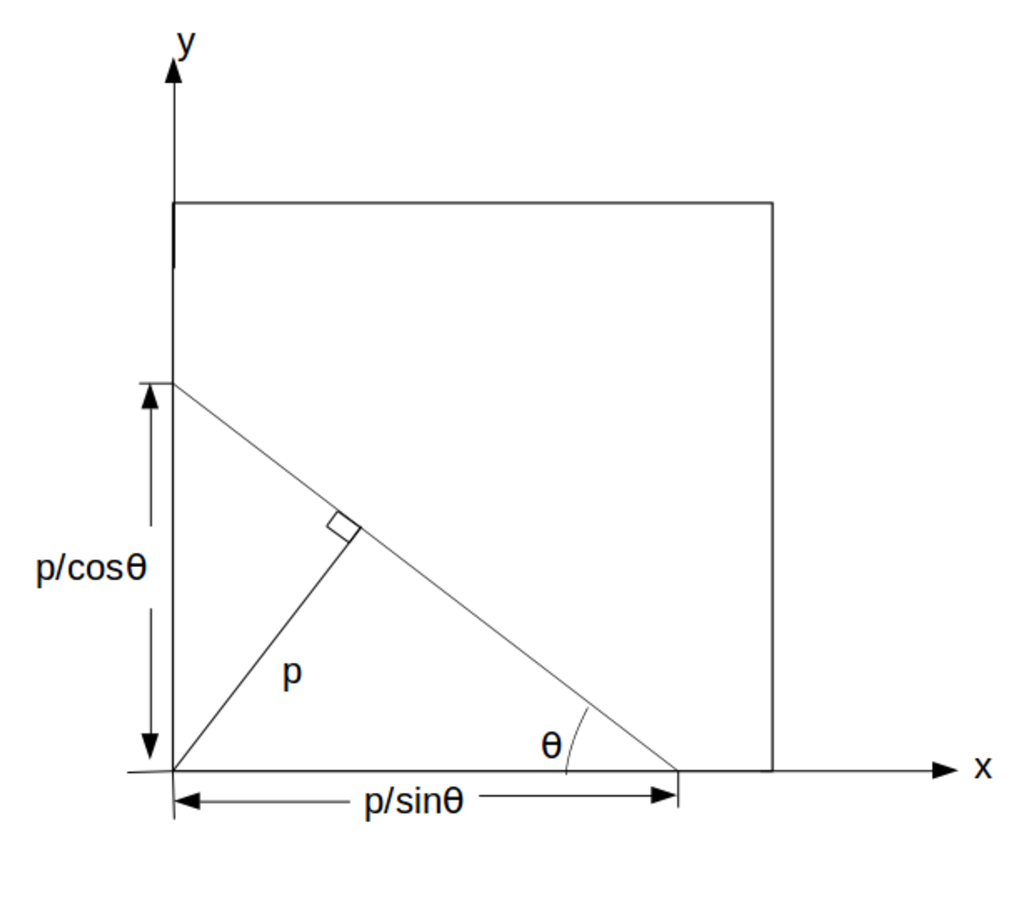
\includegraphics[scale=0.4]{normal_form.eps}
 \caption{Normal form of a line in the cell}
 \label{Fig:normal}
\end{figure}
\begin{equation}
 x\sin\theta+y\cos\theta = p
\end{equation}

Refer to Figure \ref{Fig:extrapolation} for extrapolation,

\begin{figure}%[H]
 \centering
 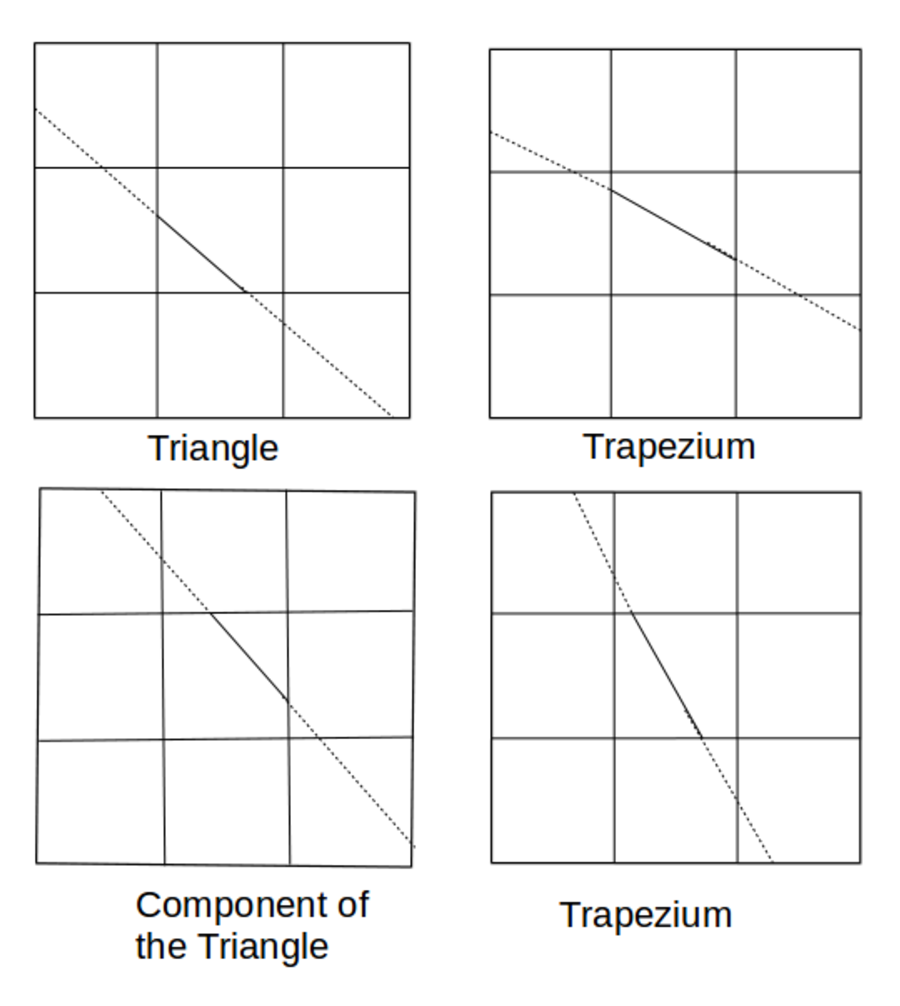
\includegraphics[scale=0.4]{extrapolate.eps}
 \caption{Extrapolation of the line in 3 X 3 cell}
 \label{Fig:extrapolation}
\end{figure}

After extrapolation the new volume fraction is calculated under each cell below the line, which is then used to calculate the norm.
\subsubsection{Step VIII: Norm Calculation}
Let the new volume fraction calculated be $\widetilde F_{r,c}$. Now the norm which is here the difference of original volume fraction and new 
volume fraction calculated after the extrapolation are squared and then summed over 3 X 3 stencil. Also, called as $L^2$ norm, \\
\begin{equation*}
 \boxed{L^2(\theta) =  \sum_{k,l=-1}^{1}(\widetilde F_{r+k,c+l}-F_{r+k,c+l})^2}
\end{equation*}

\subsubsection{Step IX : Norm Minimization}
After calculating norm the initial guess of slope and $\theta$ is changed with small step size but it should not be confused with rotation of interface or normal.
All the steps are repeated to after modifying theta and norm is again calculated. This process repeats when a minima of norm reached. And the final values of $\theta$,
shape, and quadrant are assigned to the cell.

\subsection{Advection}
The Equation \ref{Eq:advection_vof} is also solved using geometrical technique by calculating fluxes across the cells and then updating the F-field in each time step. Direct finite differencing
of this equation will lose the discontinuous property of F-field and cause smearing of interface as shown in Figure \ref{Fig:smearing}\\
% 
\underline{Flux Calculation}\\
% The flux is calculated through the wall of the cells in X an Y directions.
% for first quadrant all cases are discussed below, for all other quadrants reorientation of normal works,
% For X-Flux when velocity in x-direction, u is positive then only the right wall of the left cell will affect the flux (See Figure 11)
The flux of fluid through the walls is calculated using a graphical technique. A typical cell is shown in Figure \ref{Fig:triangle_t} and the through its right wall is calculated .
Various possibilities arise and these are discussed below.
\subsubsection{\underline{Triangle}}
For a triangle there are two cases:-\\
if $(\Delta-udt)>x_0$, Nothing will leave from the right wall \\
if $(\Delta-udt)<x_0$, A triangle leaves. \\
here $x_0$ is the value of x at $y=0$.
\begin{figure}%[H]
 \centering
 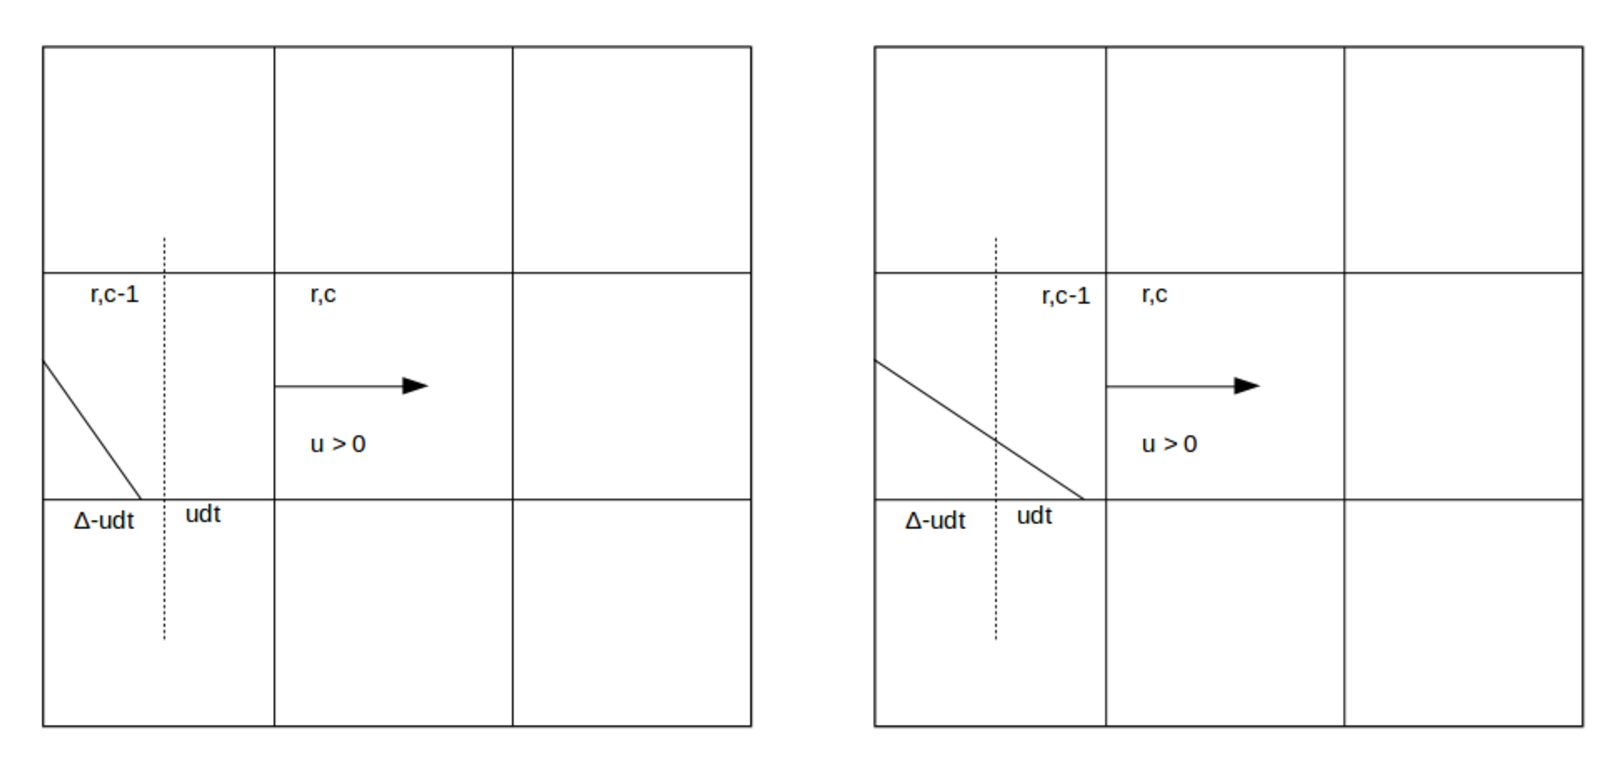
\includegraphics[scale=0.4]{ad_triangle.eps}
 \caption{Cases for a triangle in flux calculation}
 \label{Fig:triangle_t}
\end{figure}
The area of this triangle is given by,
\begin{equation*}
 \boxed{Flux = \frac{1}{2}(x_0 - \Delta + udt)^2 \tan\theta}
\end{equation*}

\subsubsection{\underline{Trapezium}}
Two types of trapezium can be in the first quadrant, $\theta<\frac{\pi}{4}$, and $\theta>\frac{\pi}{4}$, \\
(See Figure \ref{Fig:trapezium} and \ref{Fig:trapezium_cases}) \\
\begin{figure}%[H]
\centering
 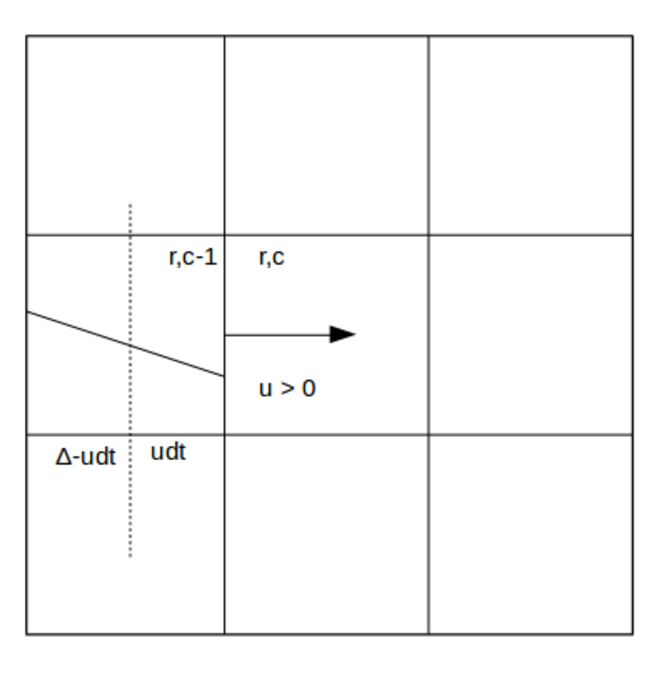
\includegraphics[scale=0.4]{ad_trapezium.eps}
 \caption{Flux calculation for trapezium for $\theta<\frac{\pi}{4}$}
 \label{Fig:trapezium}
\end{figure}

\begin{figure}%[H]
 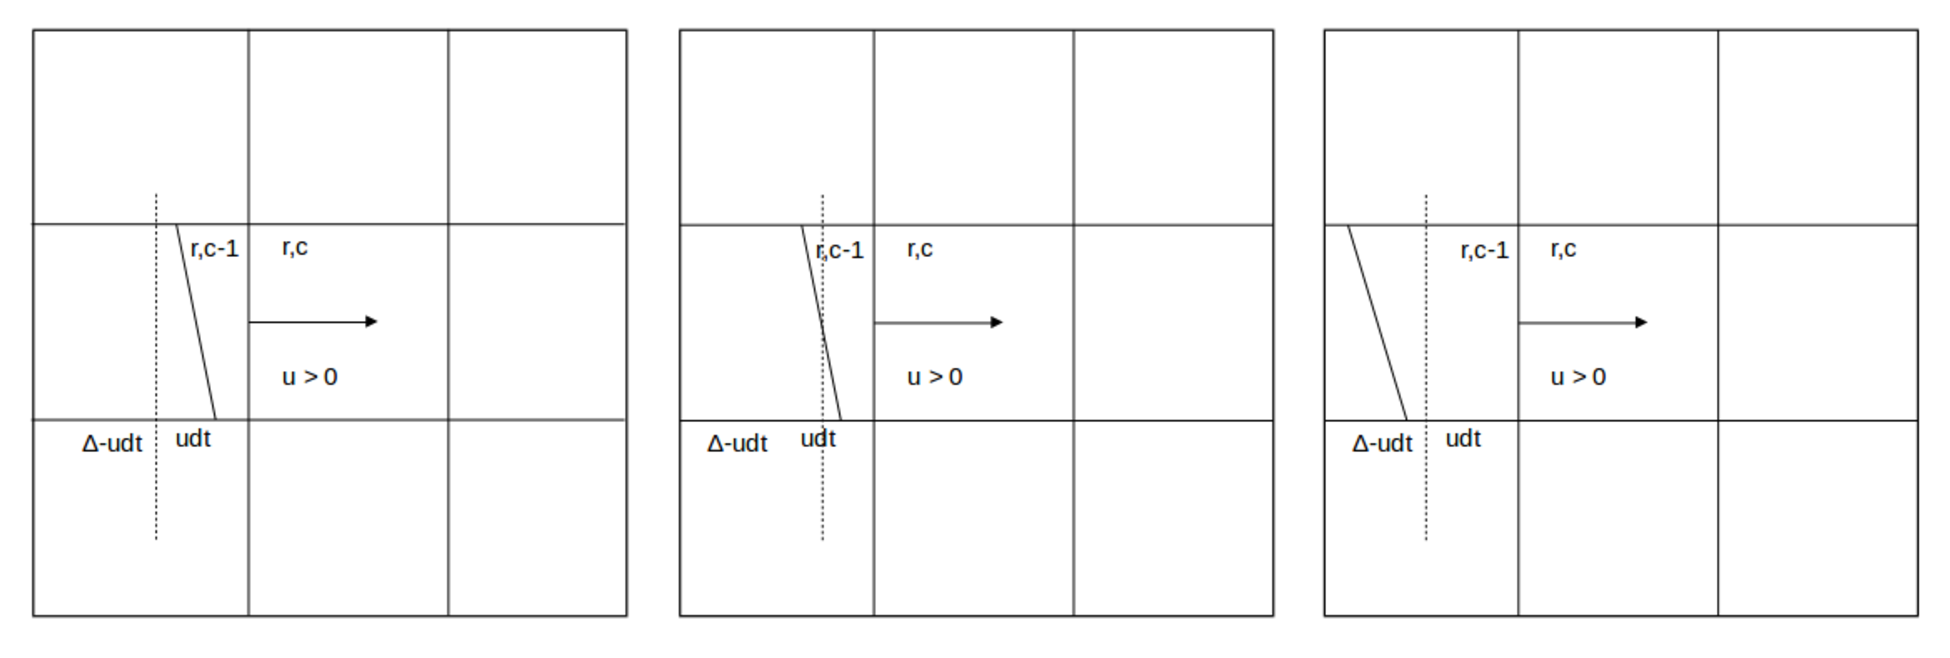
\includegraphics[scale=0.4]{ad_trap_pi4.eps}
 \caption[Different cases for flux calculation for trapezium]{(a)$(\Delta-udt)<x_{del}$, (b)$x_{del}<=(\Delta-udt)<x_0$, (c)$(\Delta-udt)>=x_0$}
 \label{Fig:trapezium_cases}
\end{figure}

For $\theta<\frac{\pi}{4}$, the only possibility is that a trapezium leaves and its area is given by,
\begin{eqnarray*}
 Flux = \frac{1}{2}( y_0 - ((\Delta - udt) \tan\theta) + y_{del} ) udt \\
\end{eqnarray*}

\begin{equation*}
 \begin{align}
 &\text{For } \theta>\frac{\pi}{4}, \\
 \text{For } &(\Delta-udt)<x_{del},  \text{ a trapezium leaves the cell and the Flux is given by,} \\
&\boxed{ Flux = \frac{\Delta}{2}(x_{del} - (2(\Delta - udt)) + x_0) }\\
 \text{For }  &x_{del}<=(\Delta-udt)<x_0,  \text{ a triangle leaves the cell and the flux is given by,} \\
&\boxed{Flux =\frac{1}{2\tan\theta} (y_0 - (\Delta - udt)\tan\theta))^2} \\
\text{For } & ((\Delta-udt))>=x_0,  \text{nothing leaves from the cell.} \\
&\boxed{Flux =0}
\end{align}
\end{equation*}

\subsubsection{\underline{Compliment of a triangle}}
For compliment of a triangle two cases arise, (See Figure \ref{Fig:compliment_triangle})
\begin{figure}%[H]
 \centering
 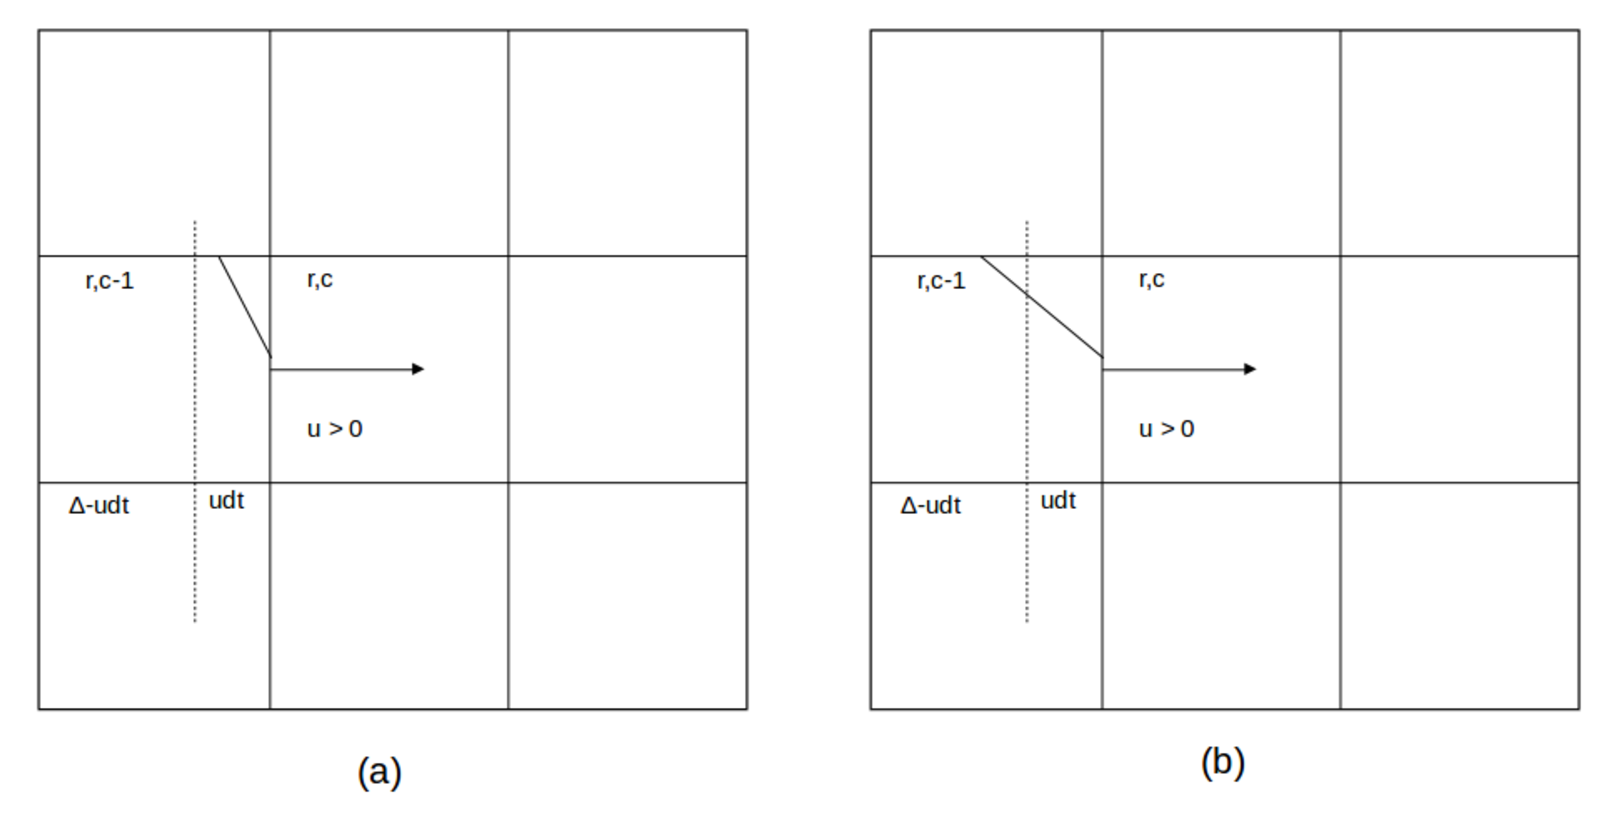
\includegraphics[scale=0.4]{ad_comp.eps}
 \caption[Different cases for flux calculation for compliment of a triangle]{(a)$(\Delta-udt) < x_{del}$, (b)$(\Delta-udt) >= x_{del}$}
 \label{Fig:compliment_triangle}
\end{figure}
\begin{equation*}
\begin{aligned}
\text{if, } \Delta -udt &< x_{del}, \text{ A 5-Sided figure leaves,  and Flux is given by,} \\
&\boxed{Flux = \Delta(x_{del} - \Delta + udt)) + \frac{1}{2}((\Delta + y_{del})(\Delta - x_{del}))} \text{ (sum of rectangle and trapezium)} \\
\text{if, } \Delta -udt &>= x_{del},  \text{ A trapezium leaves, and Flux is given by,} \\
&\boxed{Flux =  \frac{udt}{2}( y_{del} + y_0 - (\Delta - udt)\tan\theta)}
\end{aligned}
\end{equation*}

\subsection{Volume Fraction Calculation}
The fluxes calculated in the previous section are used to update the volume fractions in the cells for the next time step. For this we use \textit{Direction Split Young's method} (DSY).
\cite{Youngs1982}. In this method the order of directions is interchanged after each time step in order to avoid systematic errors. To achieve mass conservation, for this the 
basic condition is velocity divergence. In this method, the mass cannot be conserved until all directions are taken into consideration. Hence the values of volume fraction larger than unity
and less than zero may arise after first sweep which violates the restriction, $0\leqslant F\geqslant=1$ for the next sweep. This difficulty can be solved by introducing effective 
volume of the cells (\cite{Rudman1997}). But this induces risks of small under- or overshoots. Undershoot occurs when the all the volume fraction has to be fluxed out from the cell 
but it does not and cell cannot be emptied, overshoot occurs when the cell in fluxed with the volume fraction to get filled but it does not. Both occurs because of use of effective volume
in calculation of fluxes through wall. This can be resolved by using flux correction in the second sweep \cite{Lorstad2004}. The following algorithm is used to calculate the volume 
fractions for the 2D flow. \\
Effective volume(non-dimensional, characteristic area $\Delta^2$) for the $I^{st}$ sweep,
\begin{equation*}
 \delta V^I_{r,c} = 1 - \Delta t \frac{V_{out}-V_{in}}{\Delta} 
\end{equation*}
where, $\delta V^I_{r,c}$ is the effective volume after $I^{st}$ sweep. \\
Net Flux out $\Delta J_{out}$, (non-dimensional) in or out in a cell is given by,
\begin{equation*}
 \Delta J_{out} = \frac{(J_{out}-J_{in})}{\Delta^2} 
\end{equation*}

From which Volume Fraction after $I^{st}$ of the cell is given by,
\begin{equation*}
\boxed{F_{r,c}^I =  \frac{F^0 - \Delta J_{out}}{\delta V^1_{r,c}}}
\end{equation*}
where, $F^0$ and $F^I$ are the volume fractions before $I^{st}$ sweep and after $I^{st}$ sweep respectively.

For $II^{nd}$ sweep, 
\begin{equation*}
 \begin{align}
U^*_{out}  &= \frac{\Delta t}{\Delta}u_{out} \\
 \zeta &=
\begin{cases}
 \zeta_1 = \frac{J_{out}}{U^*_{out}} & \text{if} |\zeta_1-\frac{1}{2}| \geqslant  |\zeta_2-\frac{1}{2}| \\
\zeta_2 = \frac{F_{r,c}-J_{out}}{1-U^*_{out}} & \text{if} |\zeta_1-\frac{1}{2}| <  |\zeta_2-\frac{1}{2}| 
\end{cases} \\
\text{Corrected volume is given by,} \\
\delta V^{corr} &= F_{r,c} + (1-\delta V_{r,c}^I)\zeta \\
\text{Corrected outgoing flux is given by,} \\
J_{out}^{corr} &=  \delta V_{r,c}^I (J_{out}-U^*_{out}) + \delta V^{corr} U^*_{out} \\
\text{Corrected Total flux out from the cell is given by }\\
 \Delta J_{out}^{corr} &= J_{out}^{corr} - J_{in} \\
 \end{align}
 \end{equation*}
 \begin{equation*}
 \begin{align}
 \text{Final flux after last sweep is given by,}\\
 \boxed{F_{r,c}^{II} = F_{r,c}^{I} \delta V_{r,c}^I -  \Delta J_{out}^{corr}}
 \end{align}
\end{equation*}
\section{Verification}
There are standard test cases are available in the literature: \cite{Zalesak1979}, \cite{Puckett1997}, \cite{Anton2001}, \cite{Gerlach2006} etc.
These involve advecting the interface with a fixed underlying velocity field of varying degree of complexity.
Volume of Fluid method is validated by choosing three test cases from \cite{Rudman1997}, 

\begin{enumerate}
 \item \textbf{Circle in translational flow} \\
 In this test the velocity field has zero velocity gradient and it is the simplest of all the tests.
 \item \textbf{Solid body rotation of slotted circle} \\
 The test has rate of strain tensor zero and gradient of velocity only has the vorticity component with constant angular velocity at every point in space.
 \item \textbf{Circle in shear flow} \\
Vorticity tensor in this test is zero and there is only the rate of strain tensor.
\end{enumerate}

\subsection{Advection of circle in translational flow}
The algorithm is tested for the simplest case of unidirectional velocity field. Two concentric circles are used as the initial 
condition for translational test, with center at (0.75,1) and diameter of inner and outer circle is 0.4 and 0.8 respectively (Figure \ref{Fig:translational_test}).
The volume fraction scalar field is advected by two velocity fields u=1,v=0 and u=2,v=1. The refinement of the domain which is [0,4] x [0,4] is 200 x 200. The time
step is 0.005 units and advection proceeds for 500 and 504 steps for case 1 and case 2 respectively.

\begin{figure}%[H]
 \centering
 \subfloat[Initial Condition for translational test]{%
      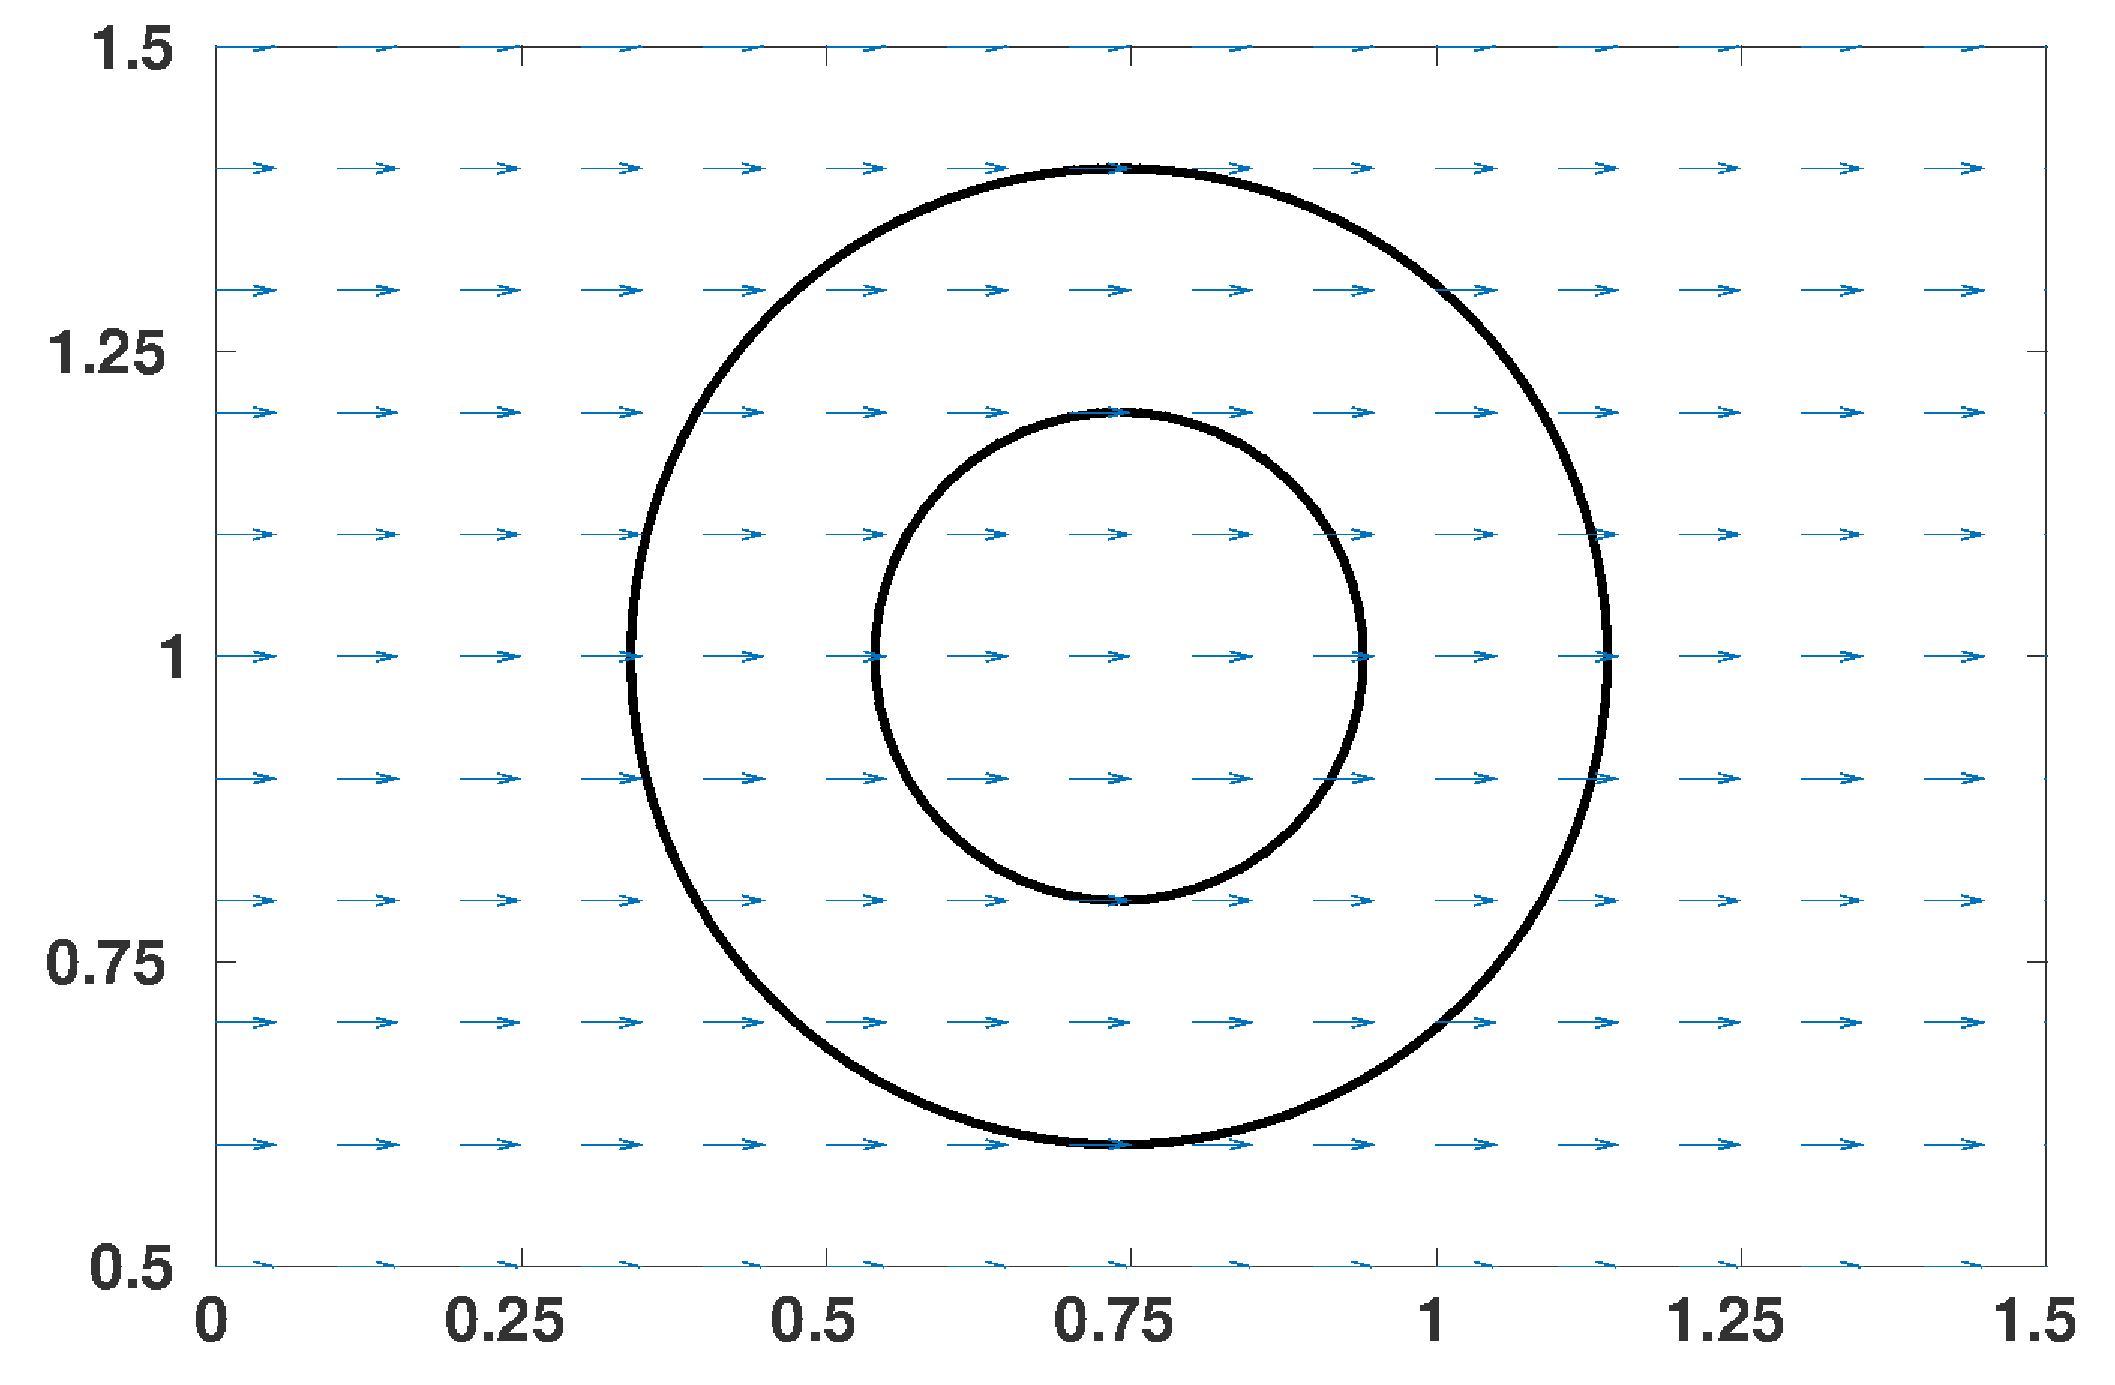
\includegraphics[width=0.5\textwidth]{IC.eps}
      }
  \subfloat[After advecting 500 steps ]{%
      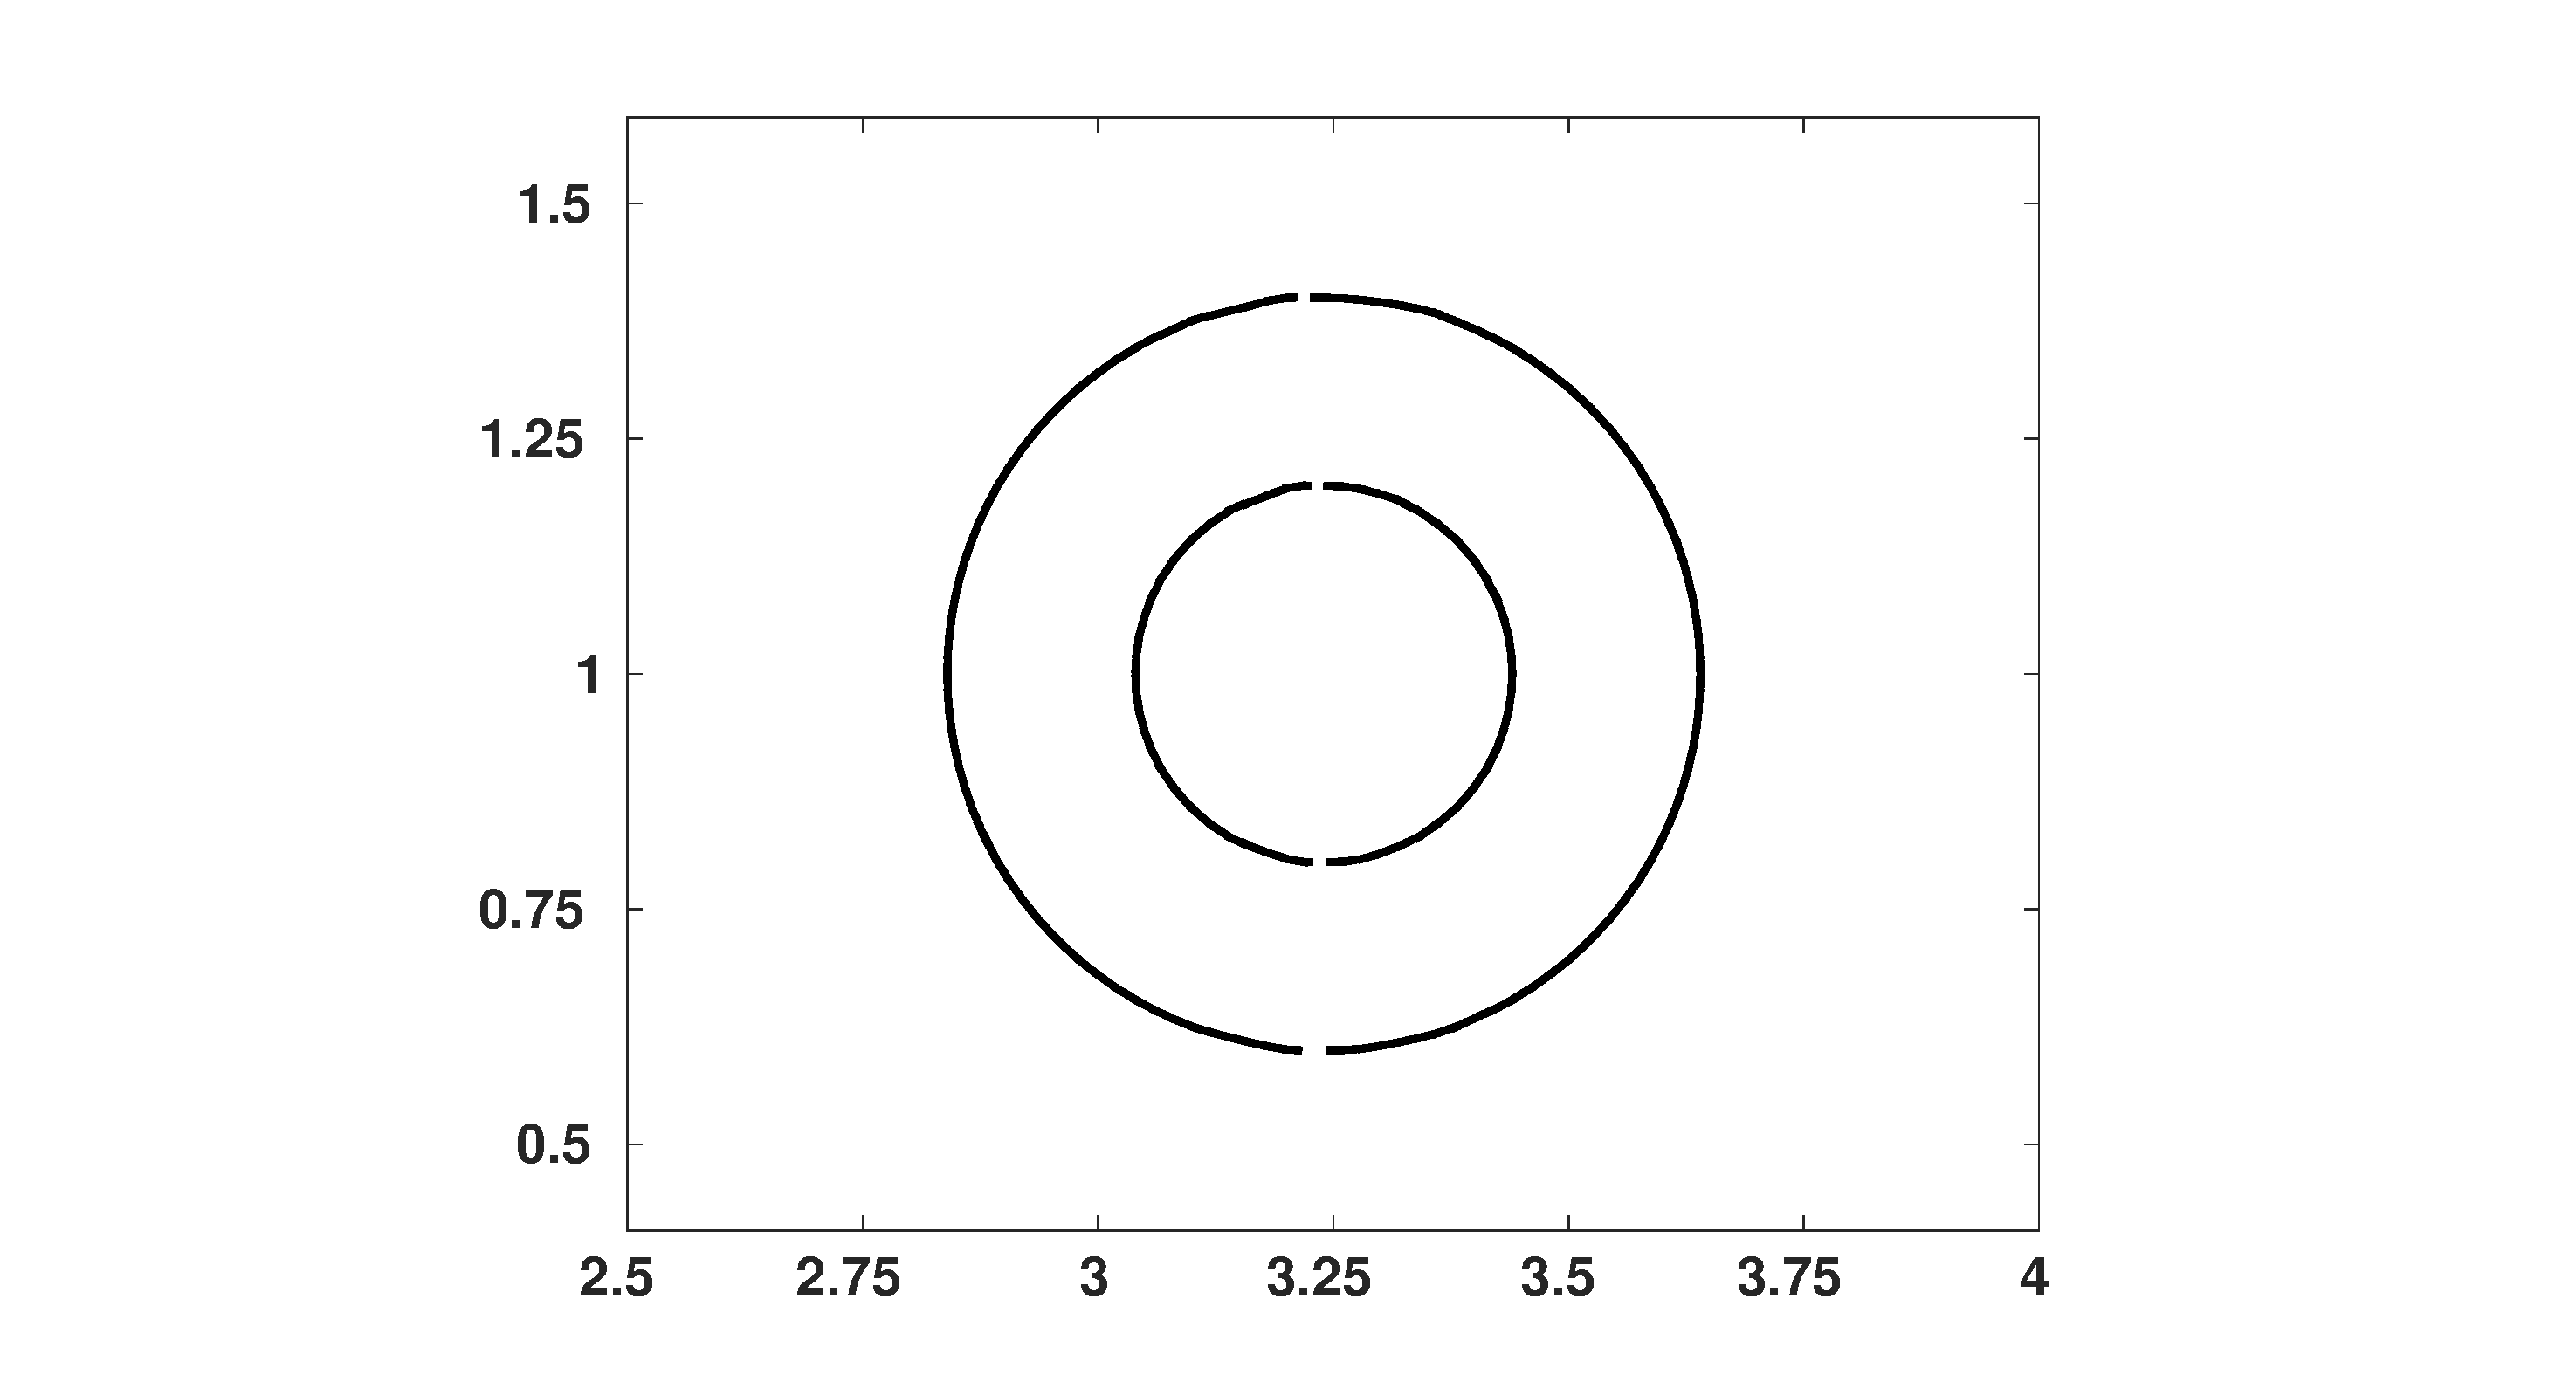
\includegraphics[width=0.5\textwidth]{final500.eps}
      }
 \caption{Advection test for velocity field u=1,v=0}
 \label{Fig:translational_test}
\end{figure}

\begin{figure}%[H]
 \centering
 \subfloat[Initial Condition for translational test ]{%
      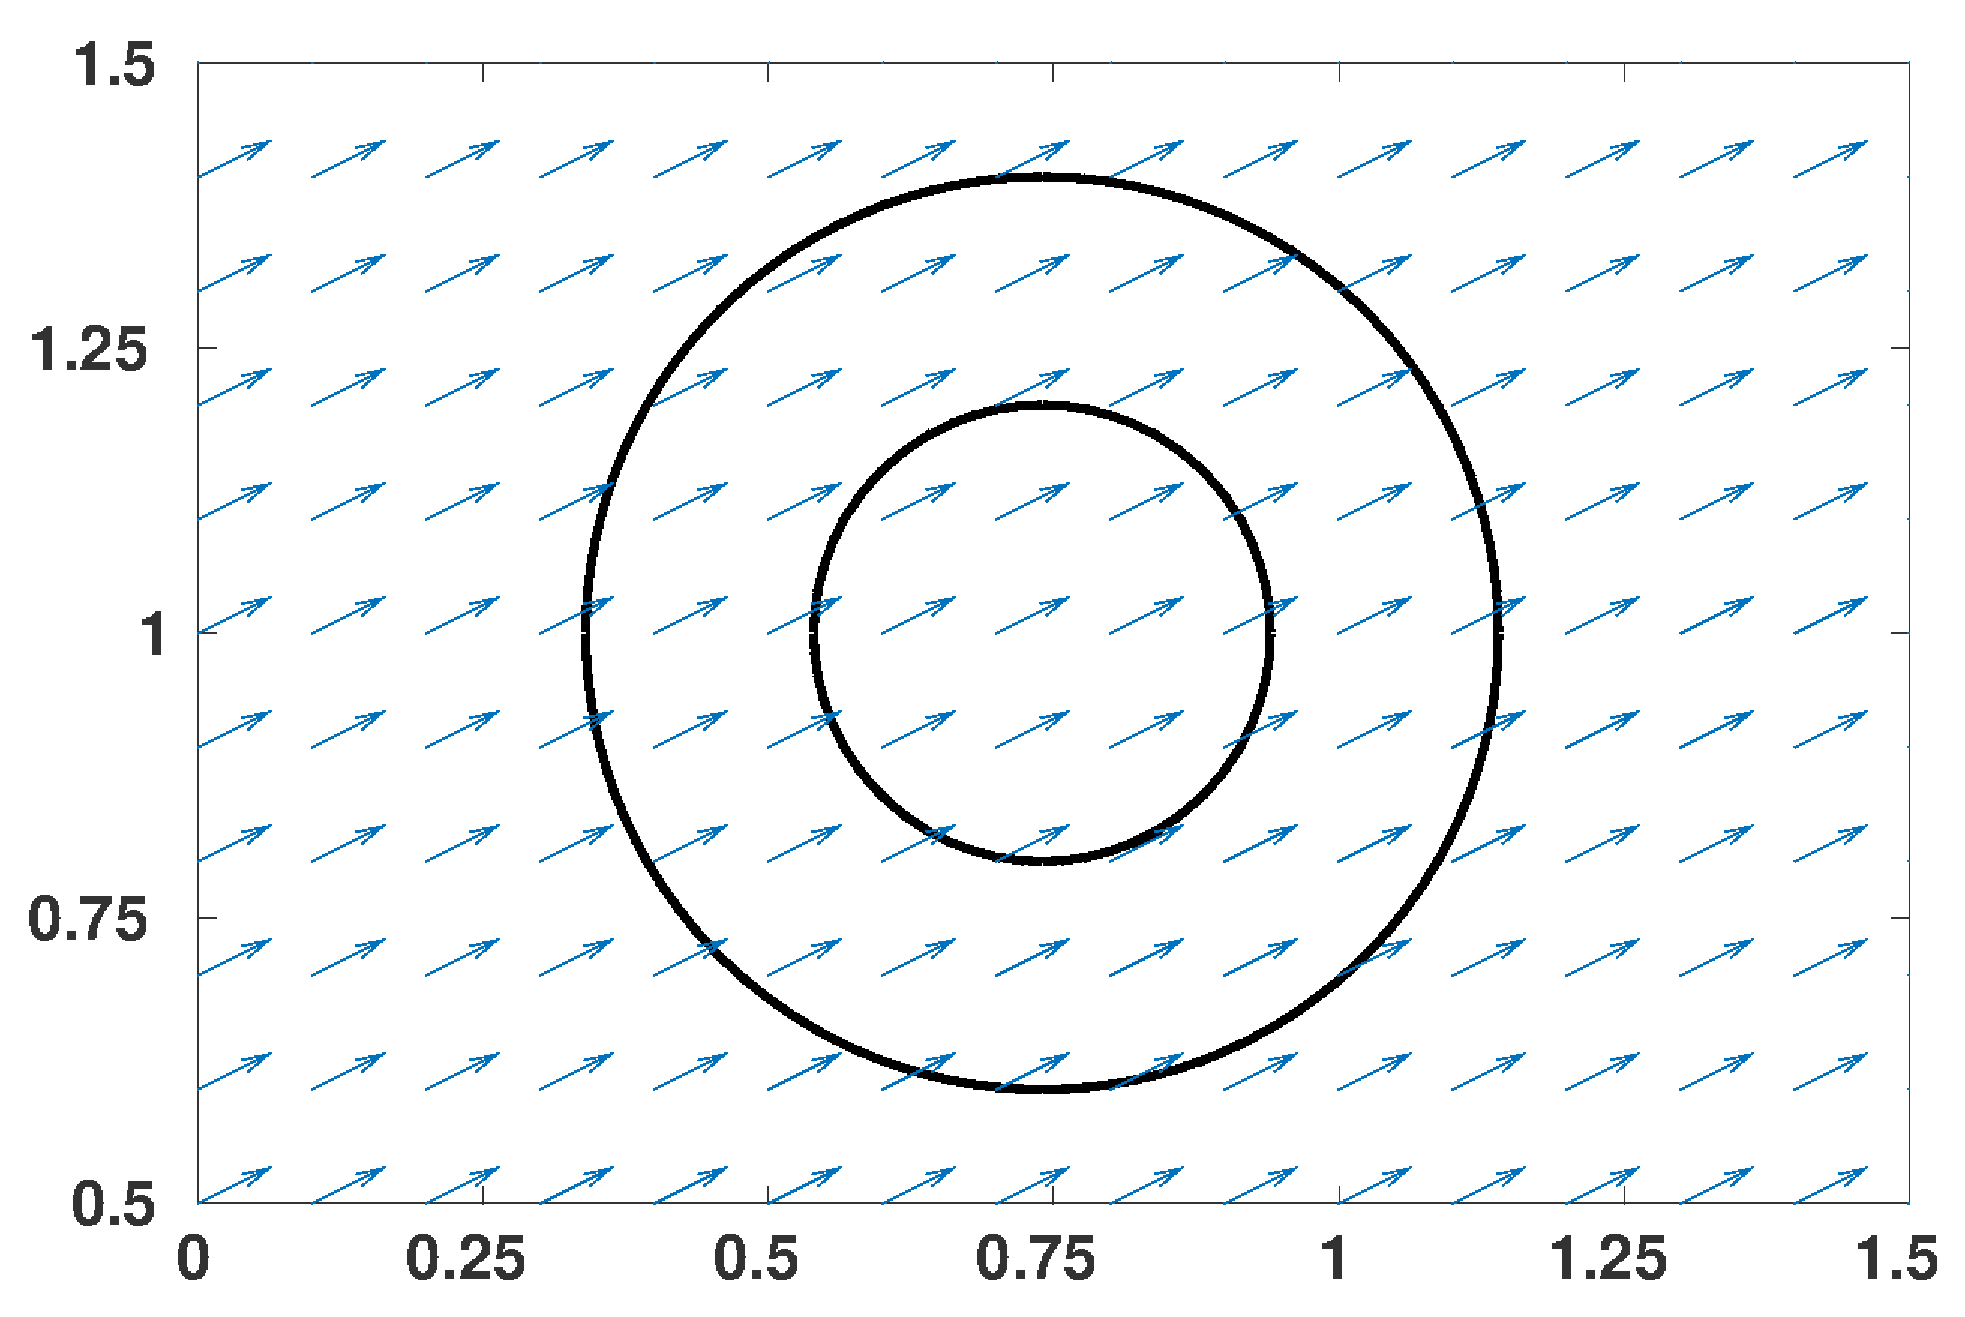
\includegraphics[width=0.5\textwidth]{IC21.eps}
      }
\subfloat[After advecting 504 steps ]{%
      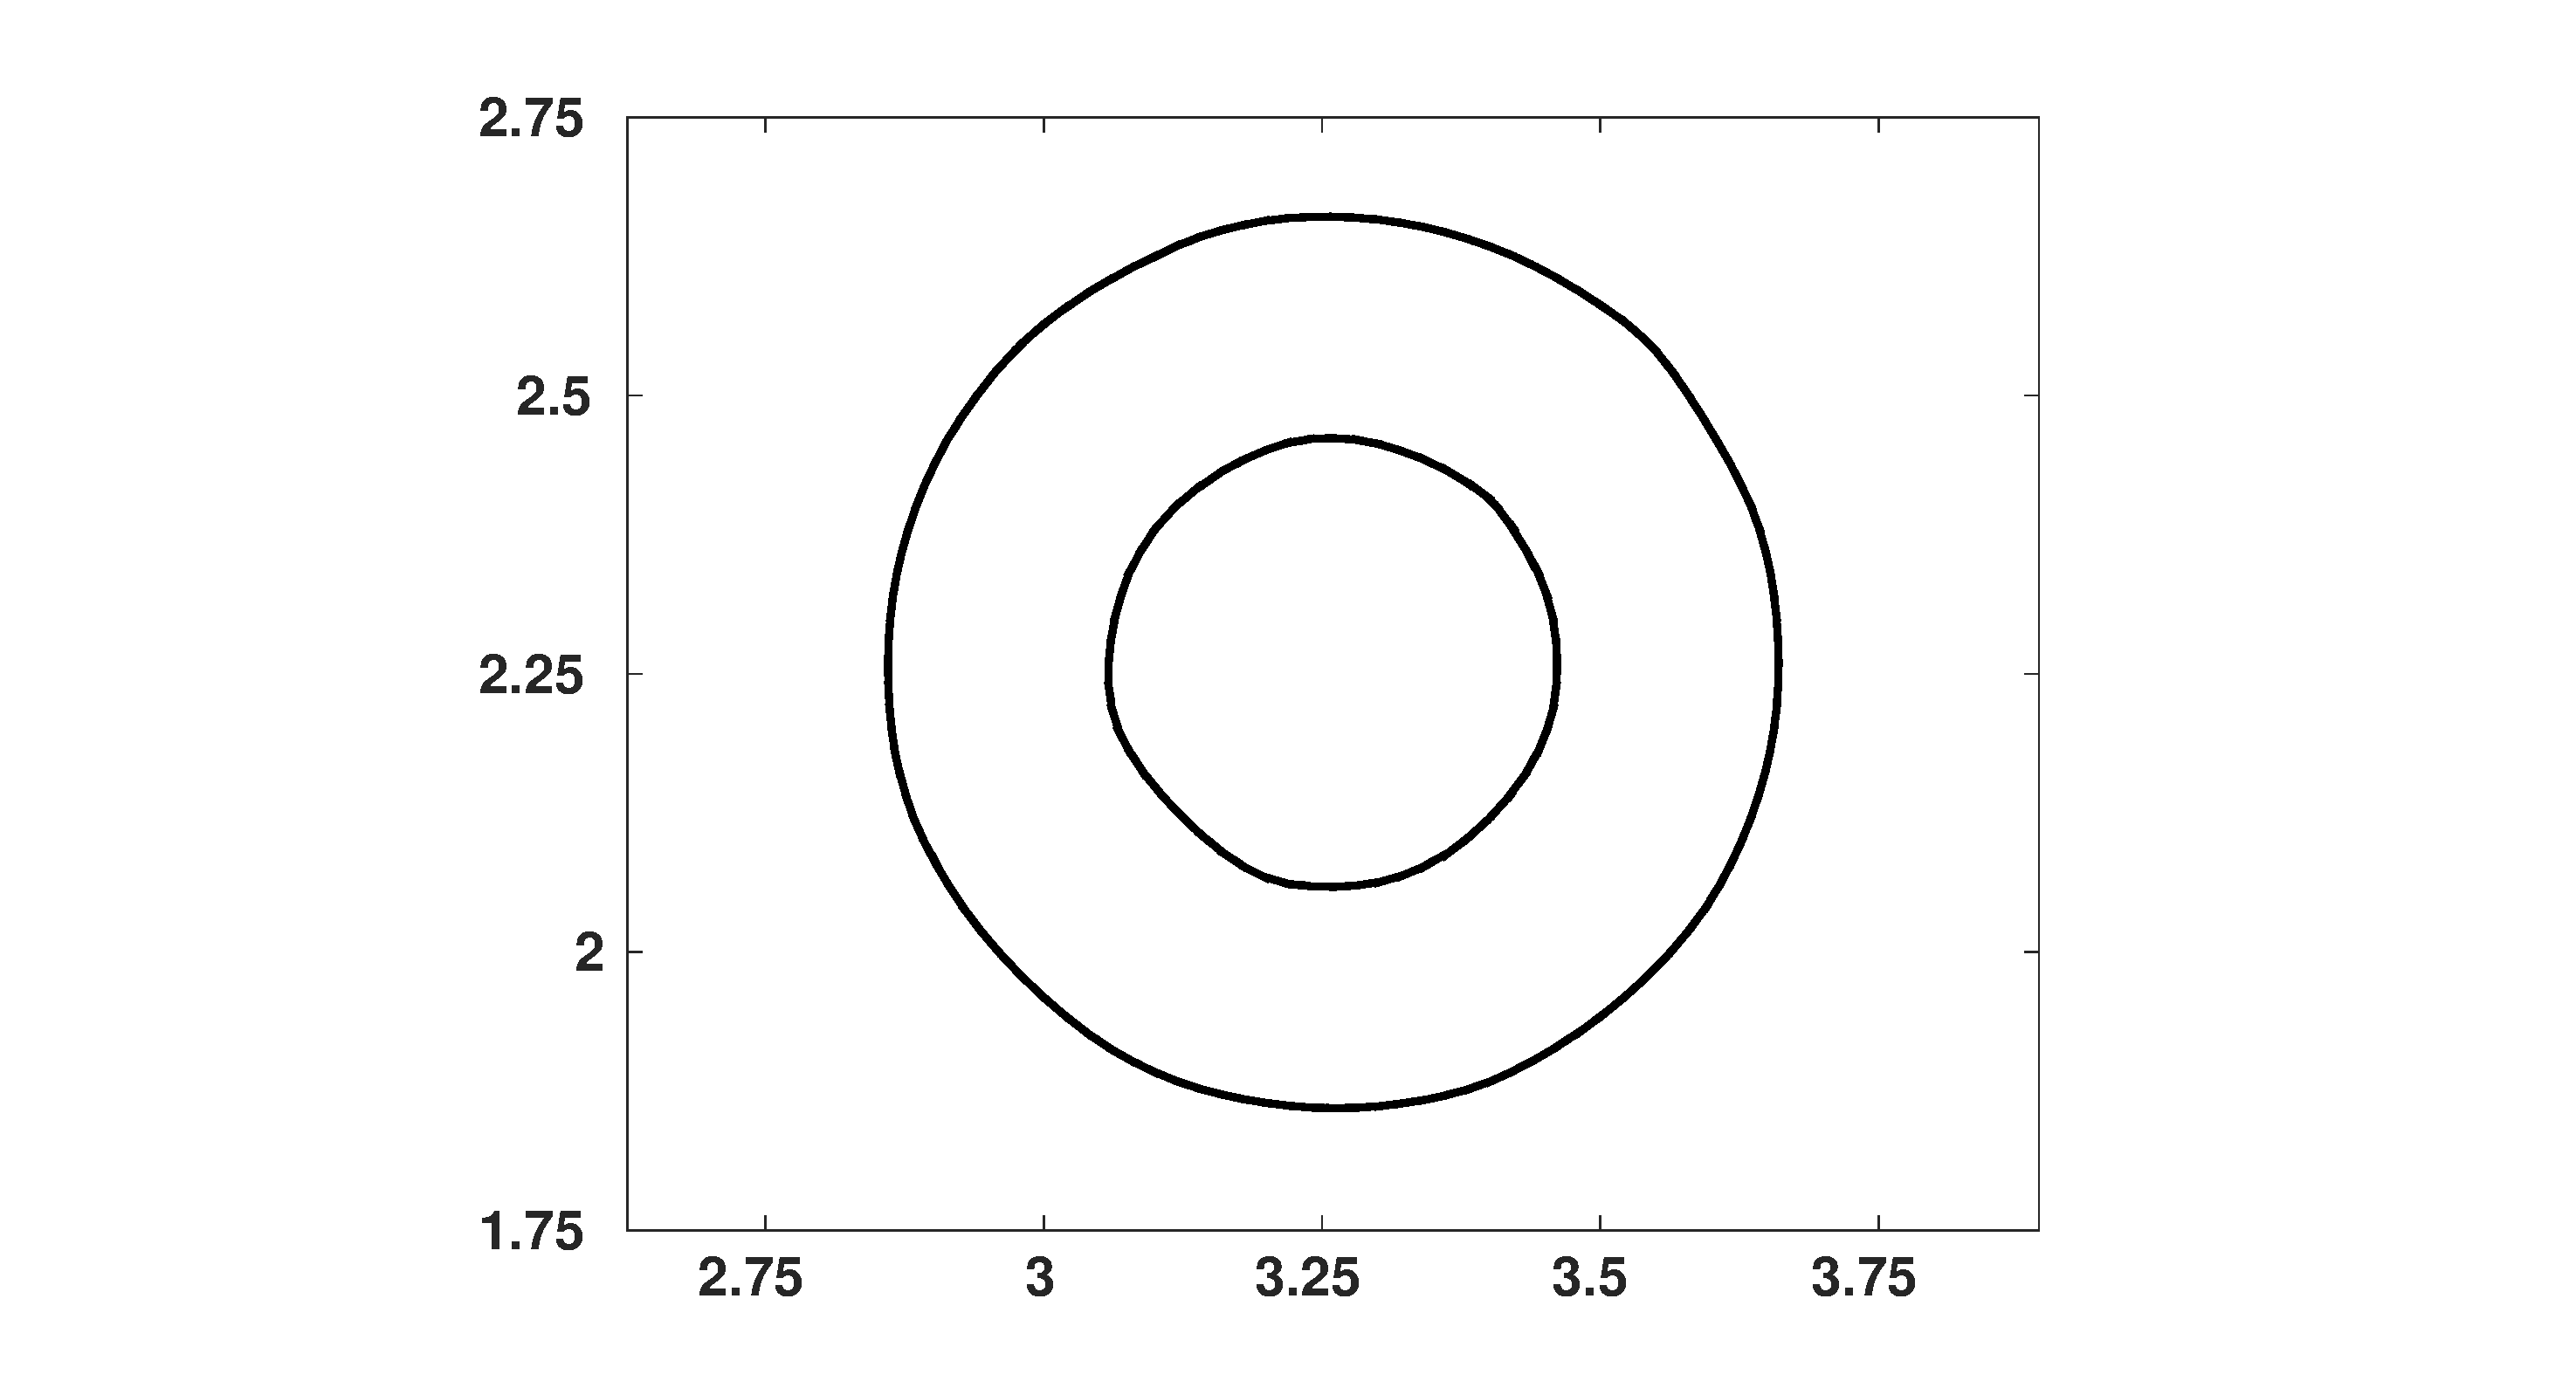
\includegraphics[width=0.5\textwidth]{final504.eps}
      }
 \caption{Advection test for velocity field u=2,v=1}
\end{figure}

\subsection{Advection test for solid body rotation}
For solid body rotation test a slotted circle configuration is taken from \cite{Zalesak1979}, the center of slotted circle is at
(2.0,2.75) and diameter is 1.0. The length and width of slot is 0.6 and 0.12 respectively.(Figure \ref{Fig:rotation} and \ref{Fig:rotation2})  
The refinement of the domain which is [0,4] x [0,4] is 200 x 200 . A velocity field is given by $u=-\Omega(y-y_0),v=\Omega(x-x_0)$, 
where axis of rotation passes through the $(x_0,y_0)$ and normal to the x-y plane. $\Omega$ is the angular velocity. 
Here $\Omega = 0.5$ and $(x_0,y_0)$ is $(2,2)$. The time step is 0.005.
\begin{enumerate}
 \item Domain: [0,4] x [0,4]
 \item Grid Size: 200 x 200
 \item Radius of circle :0.5
 \item Center : (2.0,2.75)
 \item Velocity field:  $u=-0.5(y-2),v=0.5(x-2)$
\end{enumerate}

% 
\begin{figure}
  \subfloat[After advecting 628 steps ]{%
      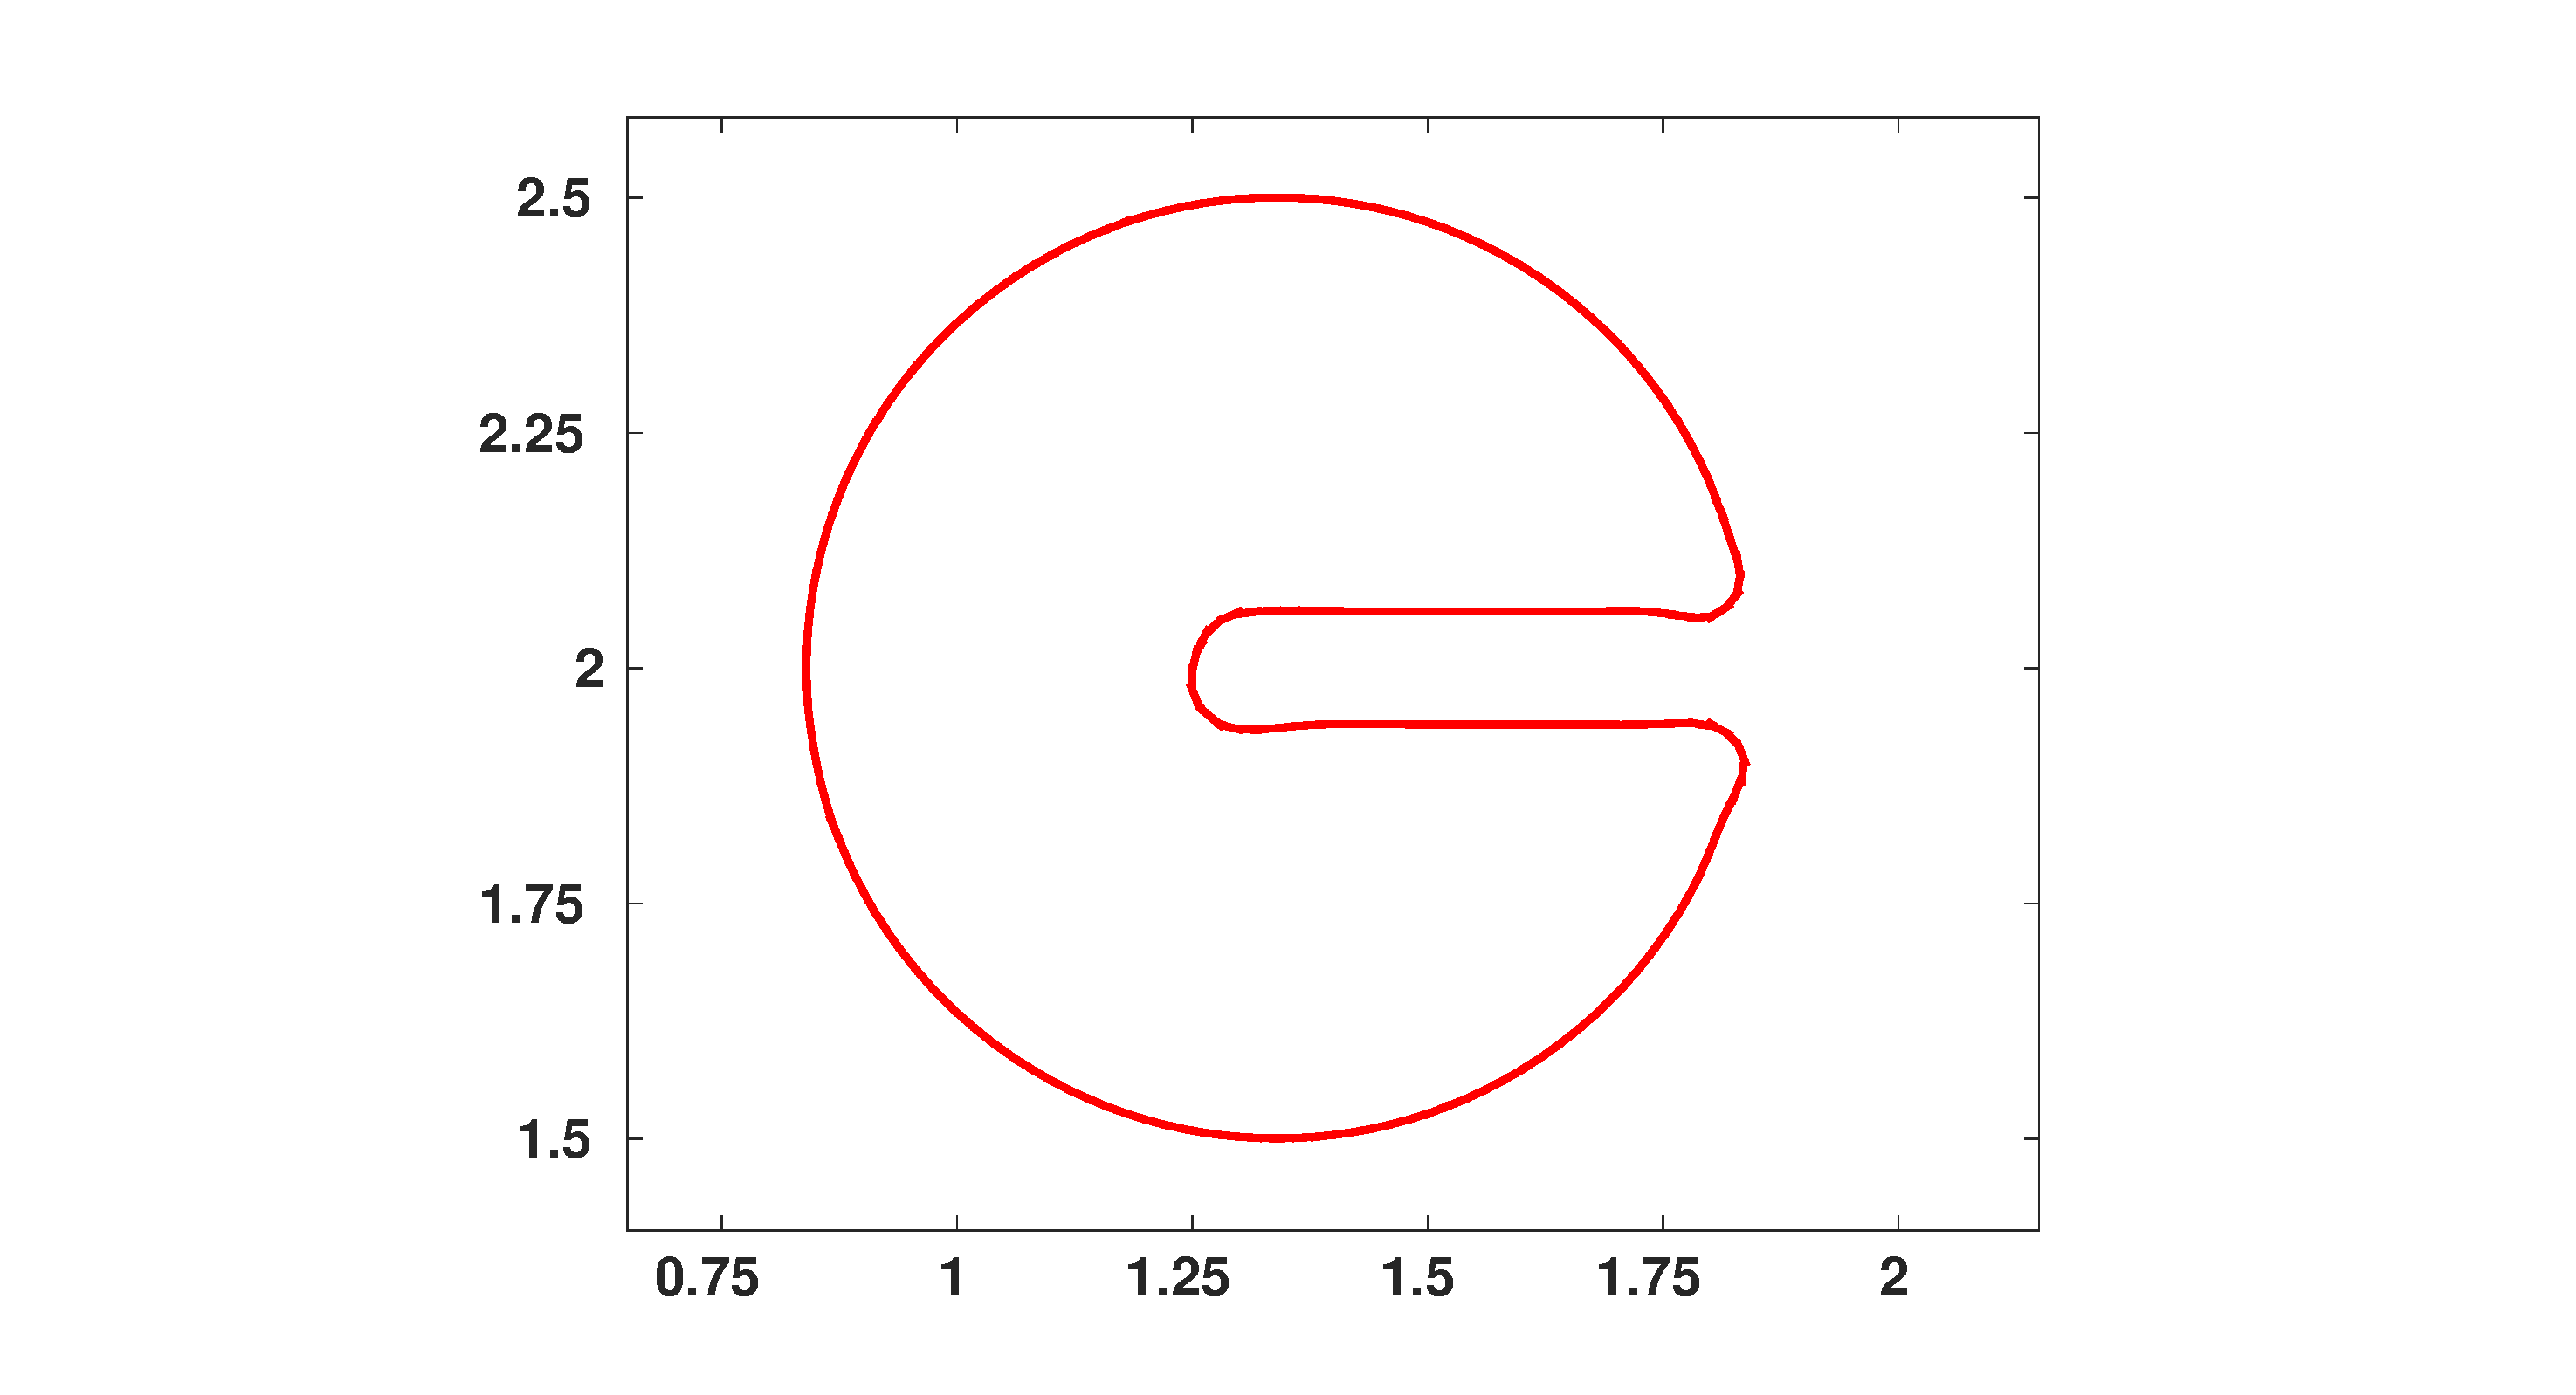
\includegraphics[width=0.5\textwidth]{SC_628.eps}
      }
     \subfloat[After advecting 1256 steps ]{%
      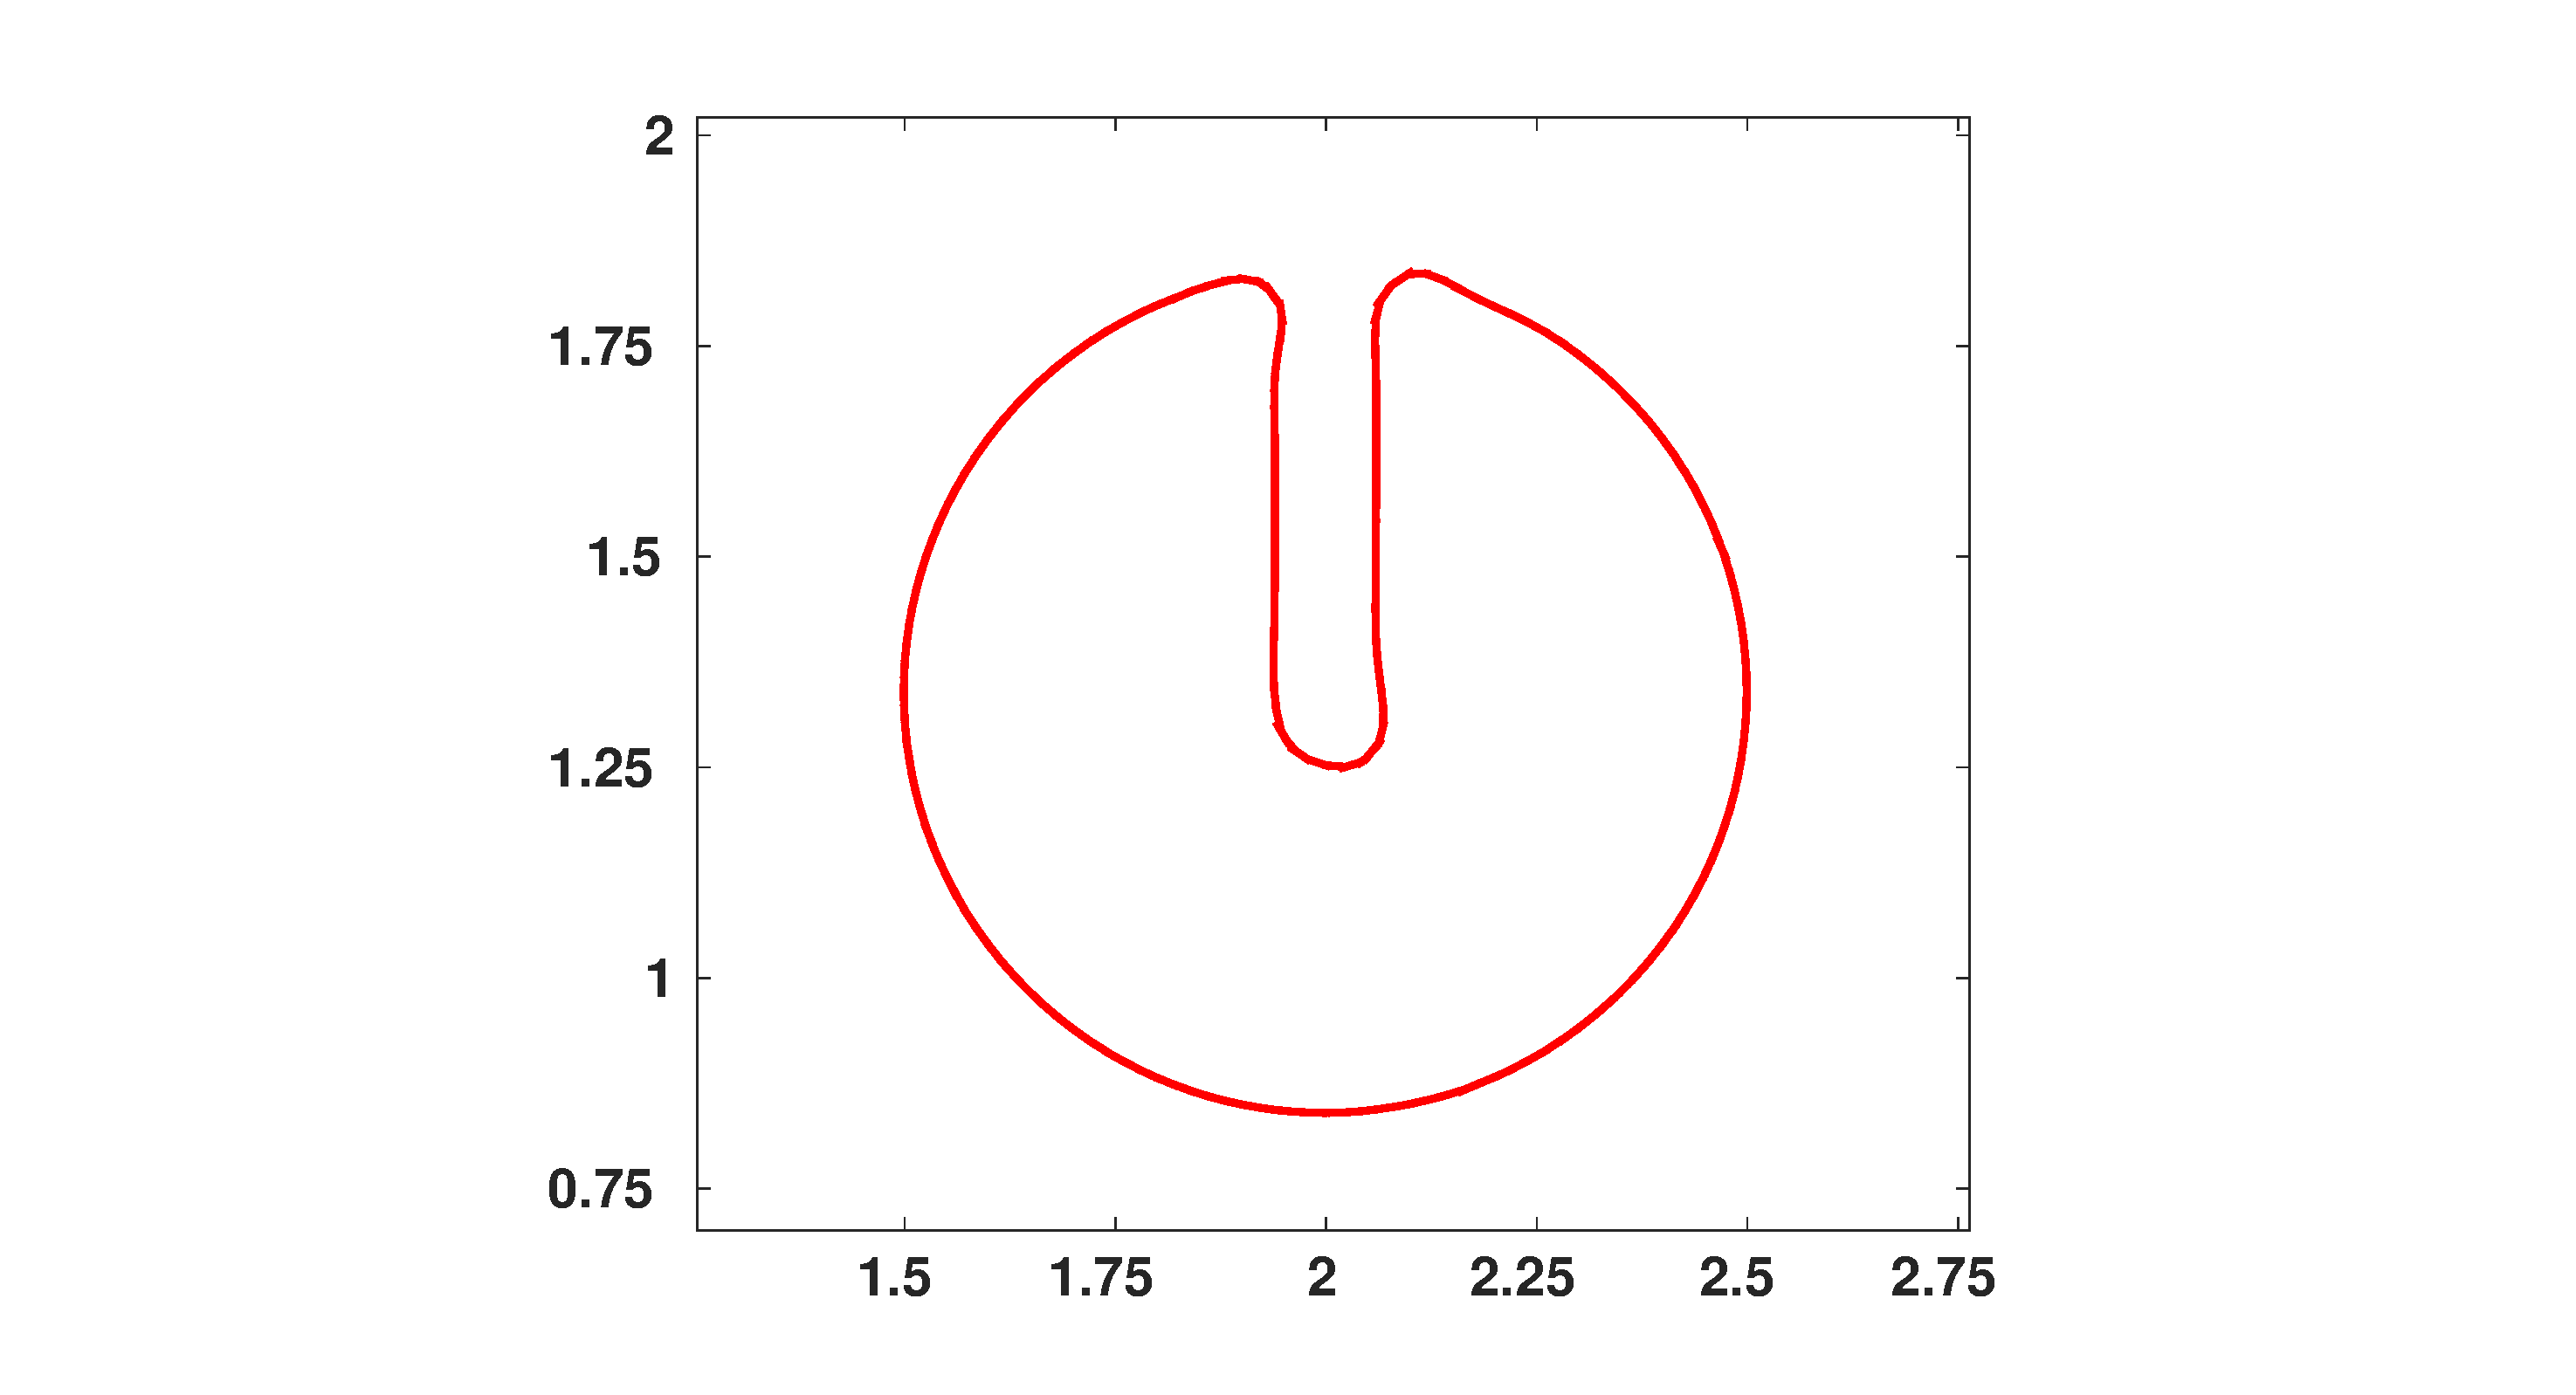
\includegraphics[width=0.5\textwidth]{SC_1256.eps}
      }\\
        \subfloat[After advecting 1885 steps ]{%
      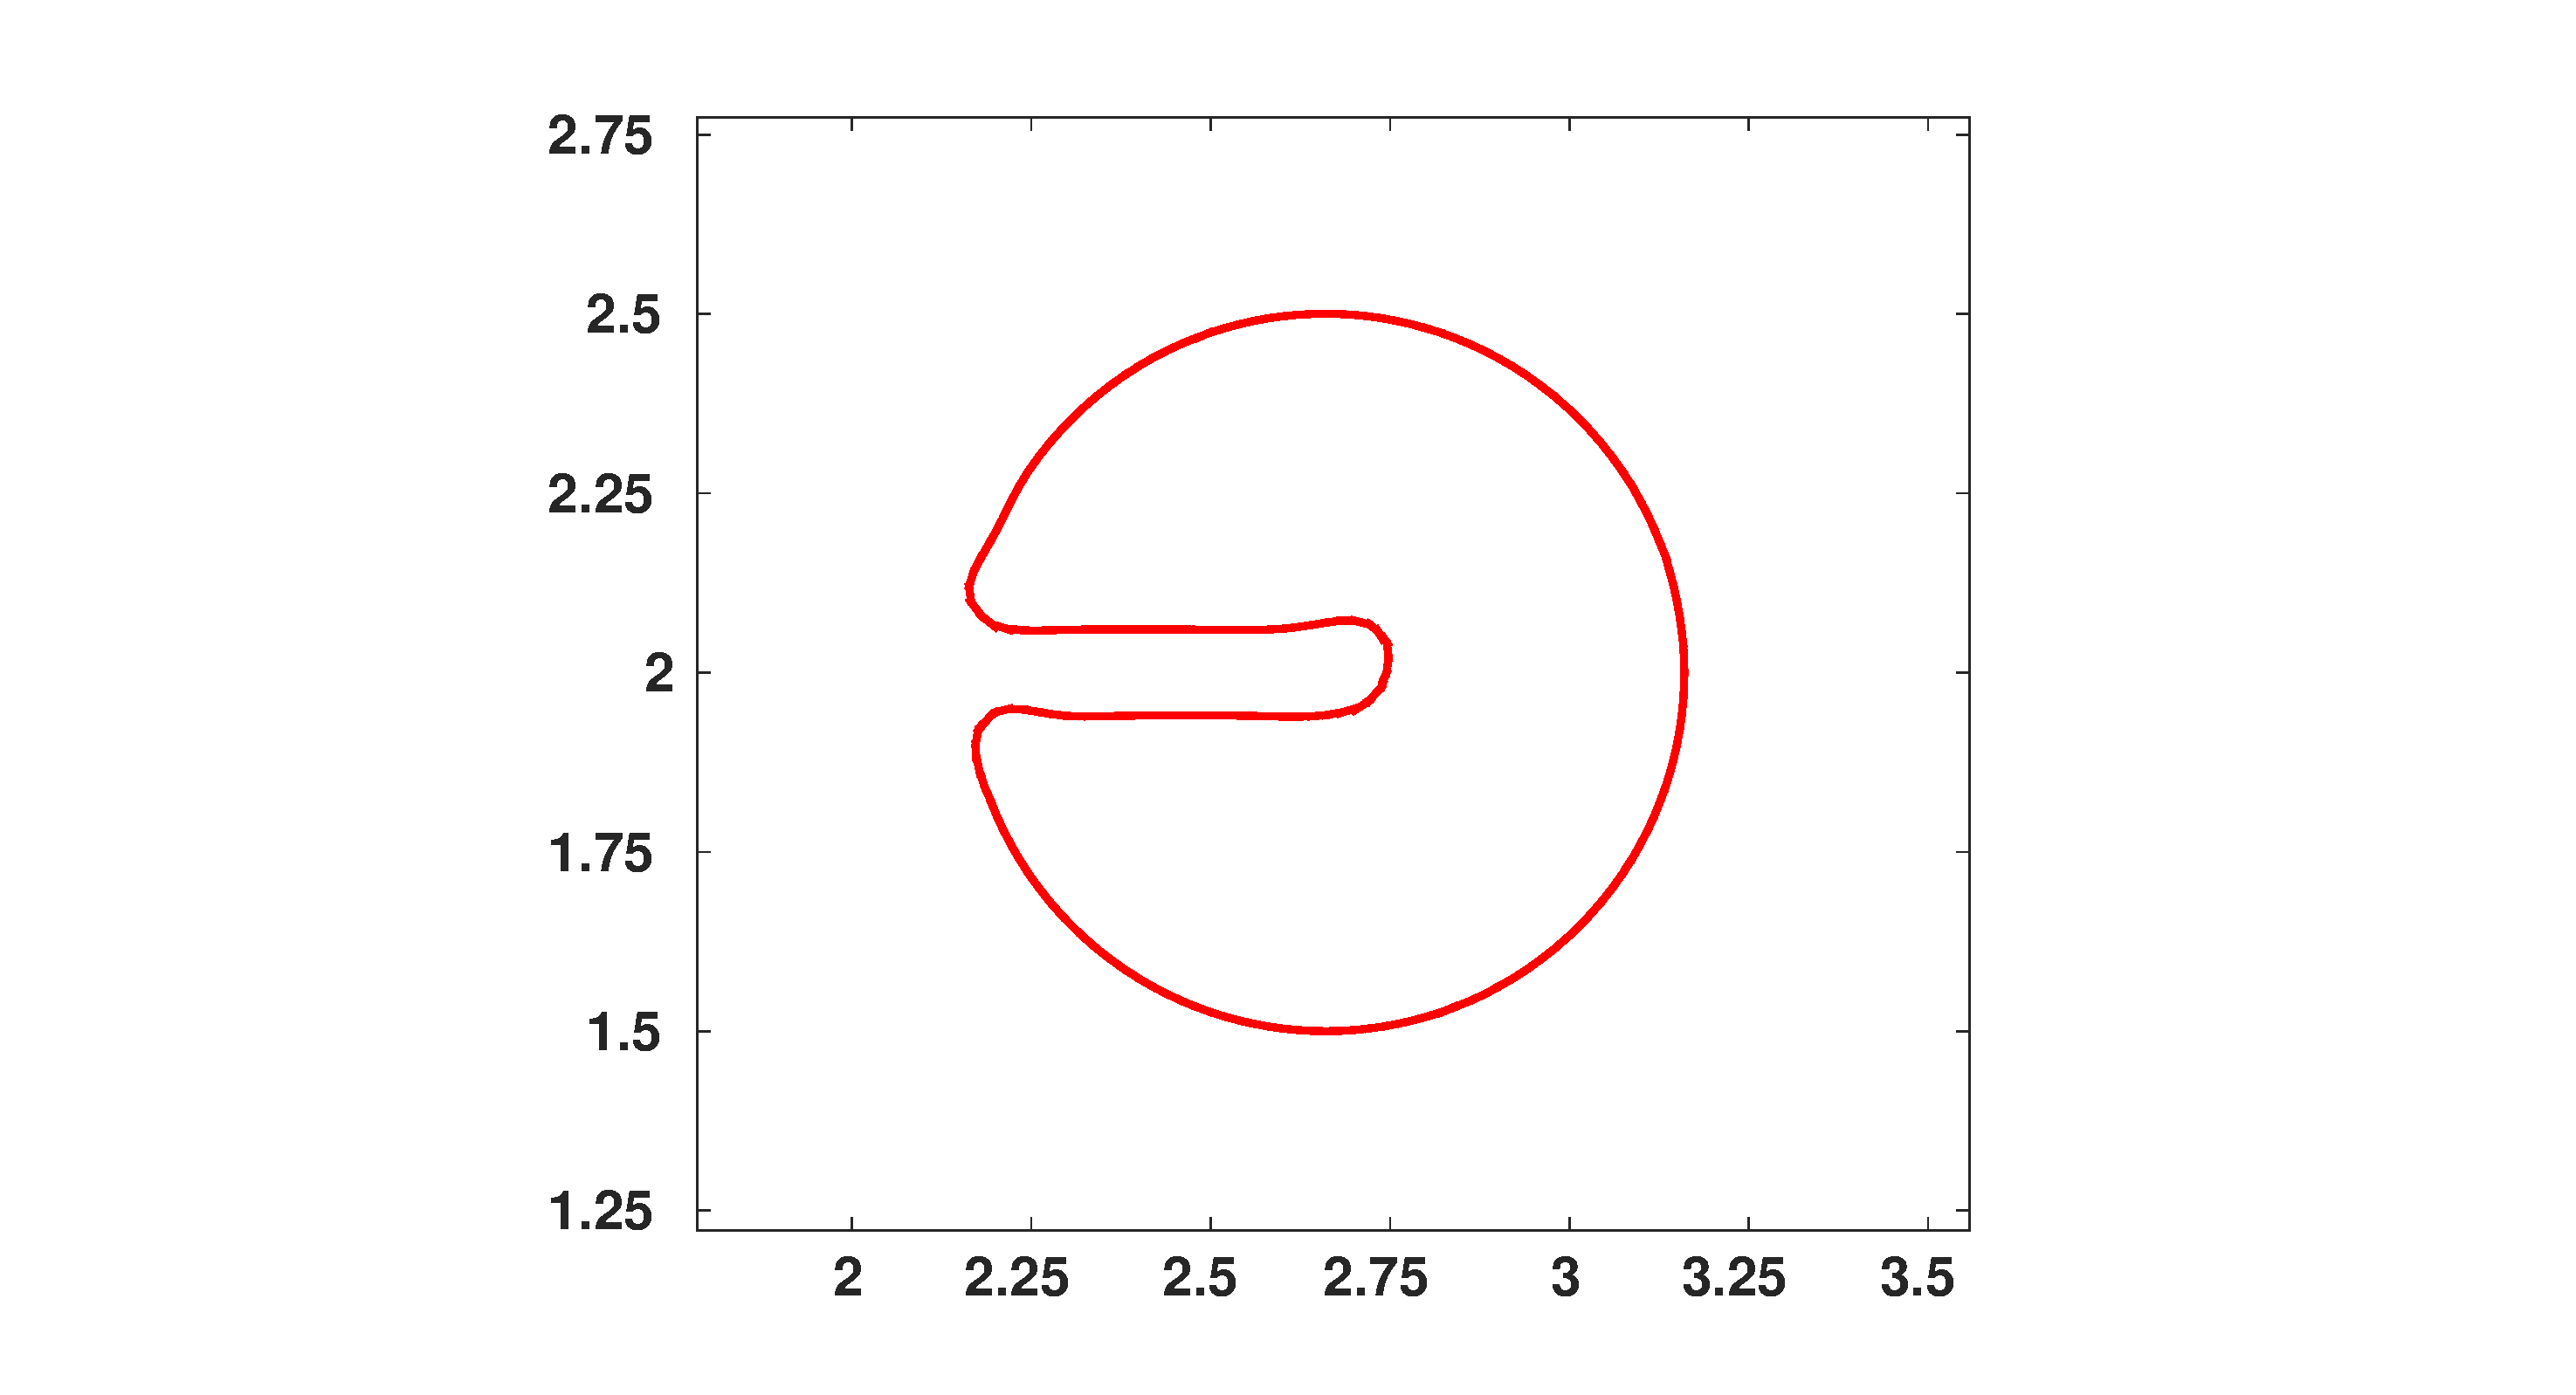
\includegraphics[width=0.5\textwidth]{SC_1885.eps}
      }
        \subfloat[After advecting 2513 steps ]{%
      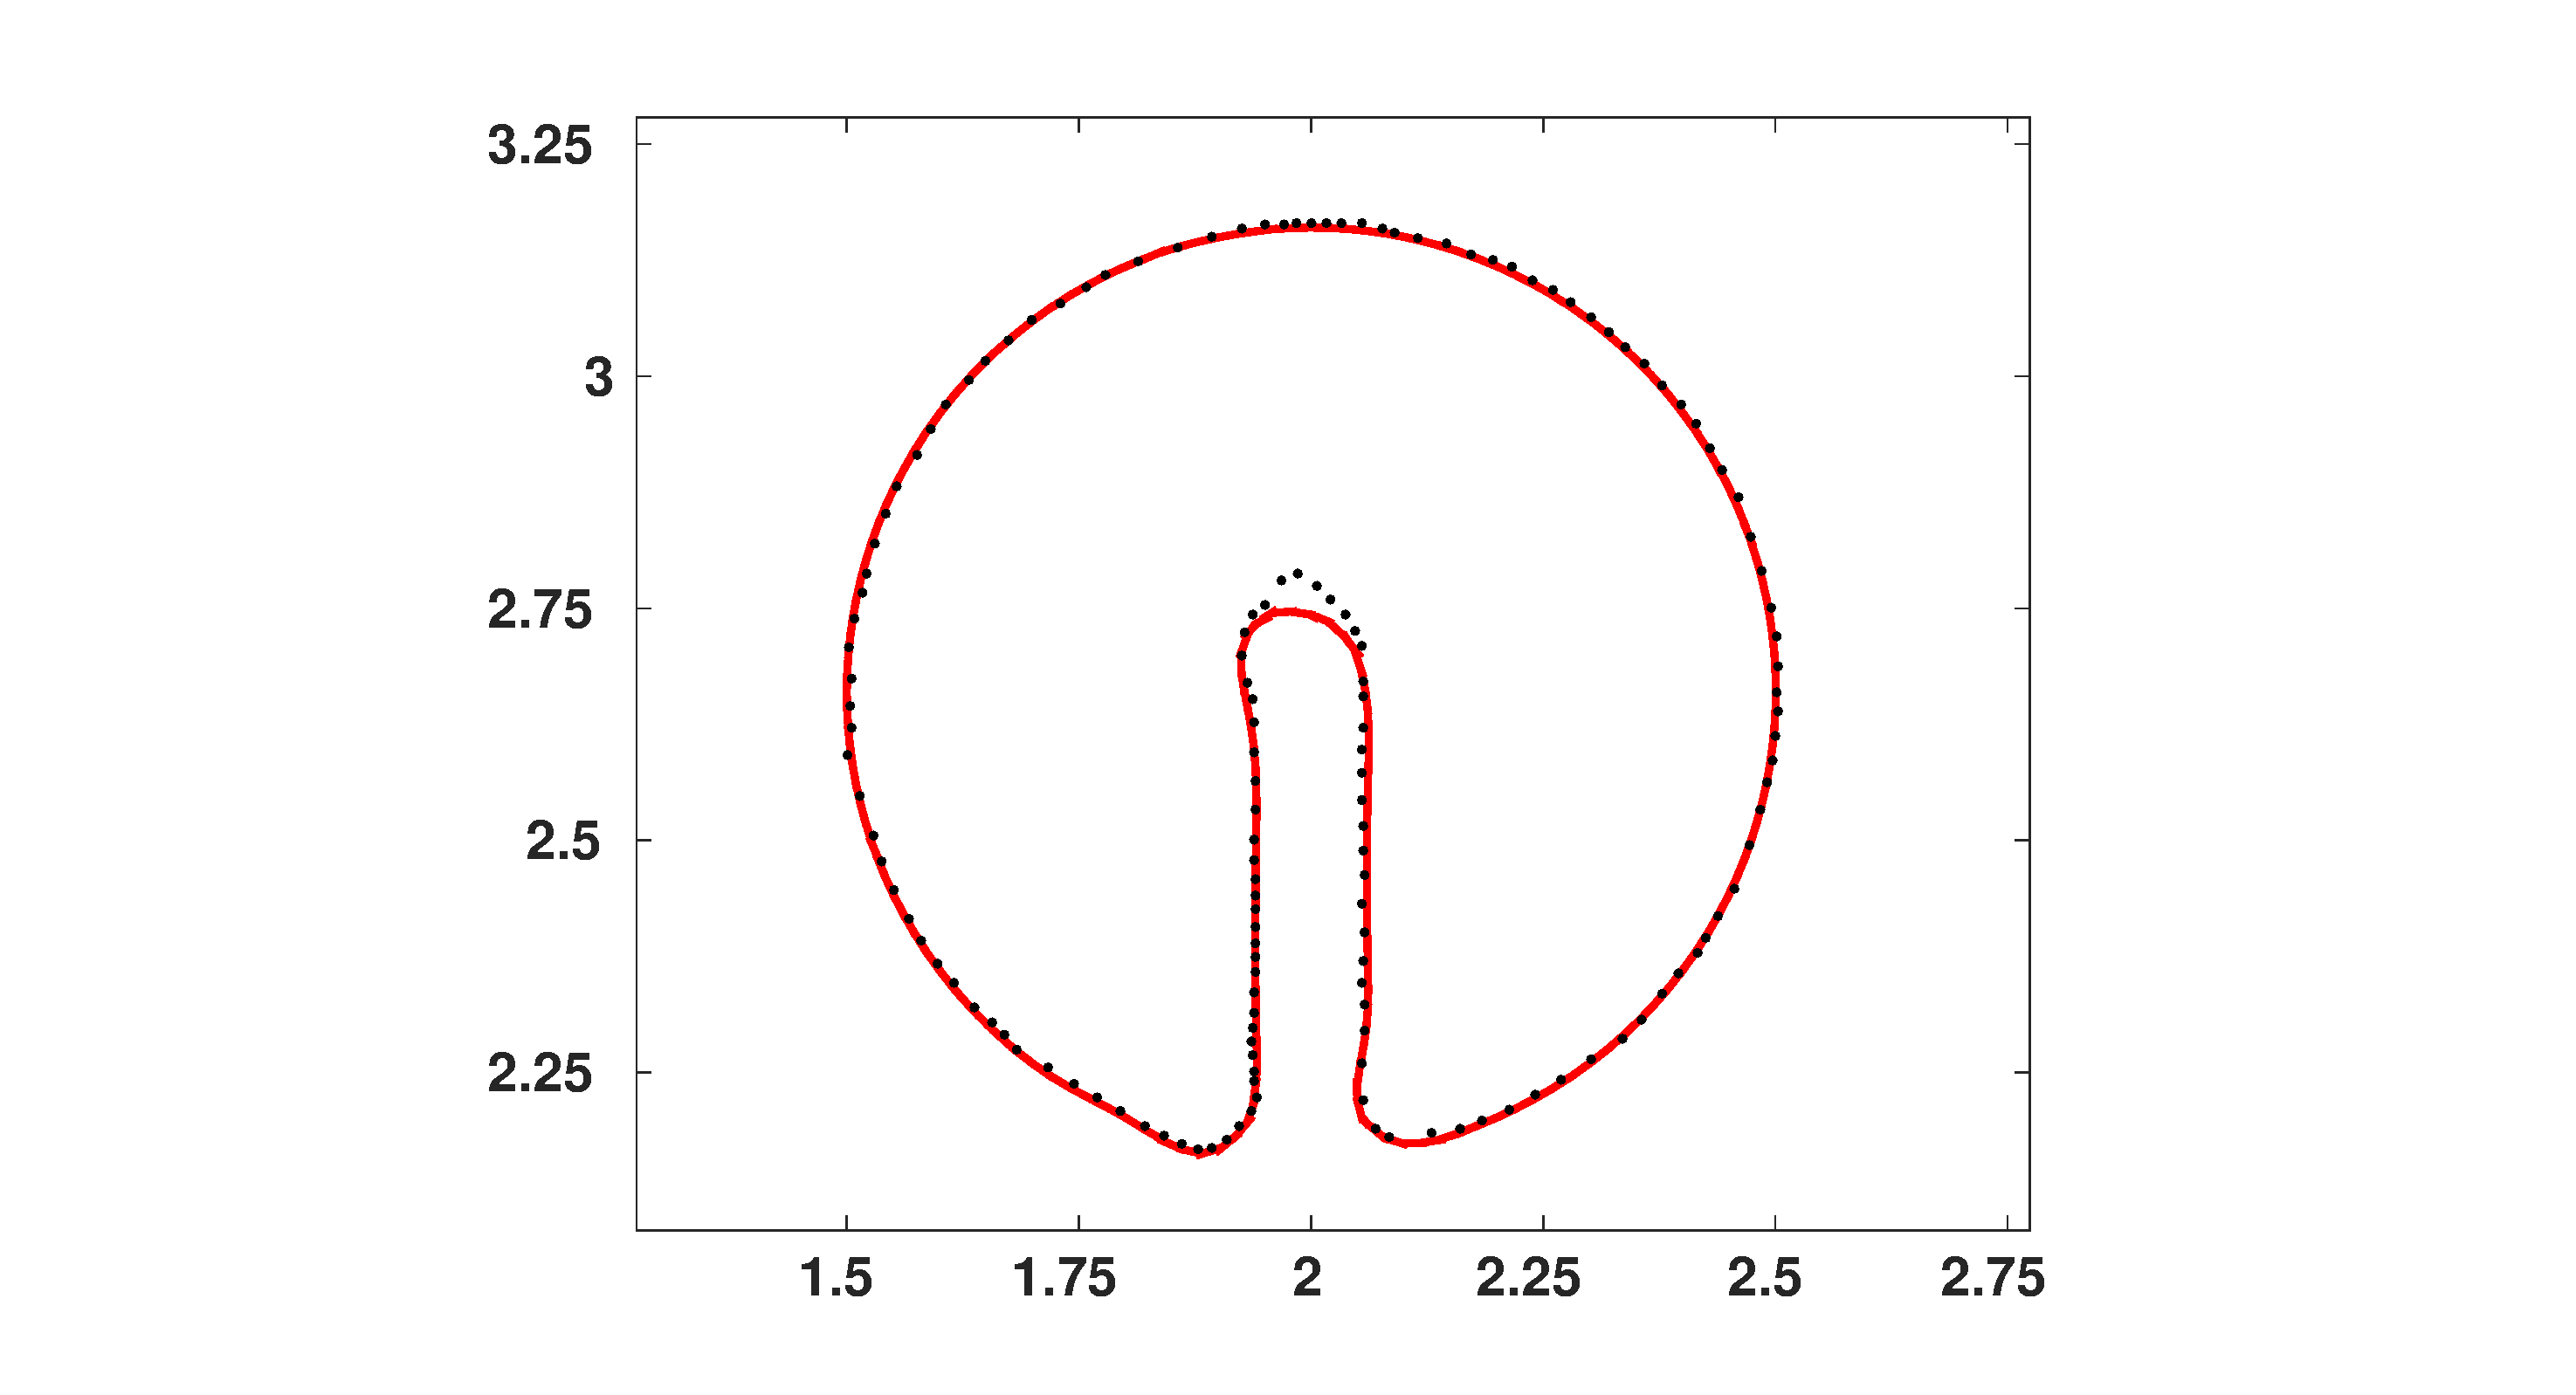
\includegraphics[width=0.5\textwidth]{SC_2513.eps}
      }
 \caption{Advection test result for solid body rotation}
 \label{Fig:rotation2}
\end{figure}
% 
\begin{figure}
 \centering 
 \subfloat[Initial Condition for solid body rotation test ]{%
      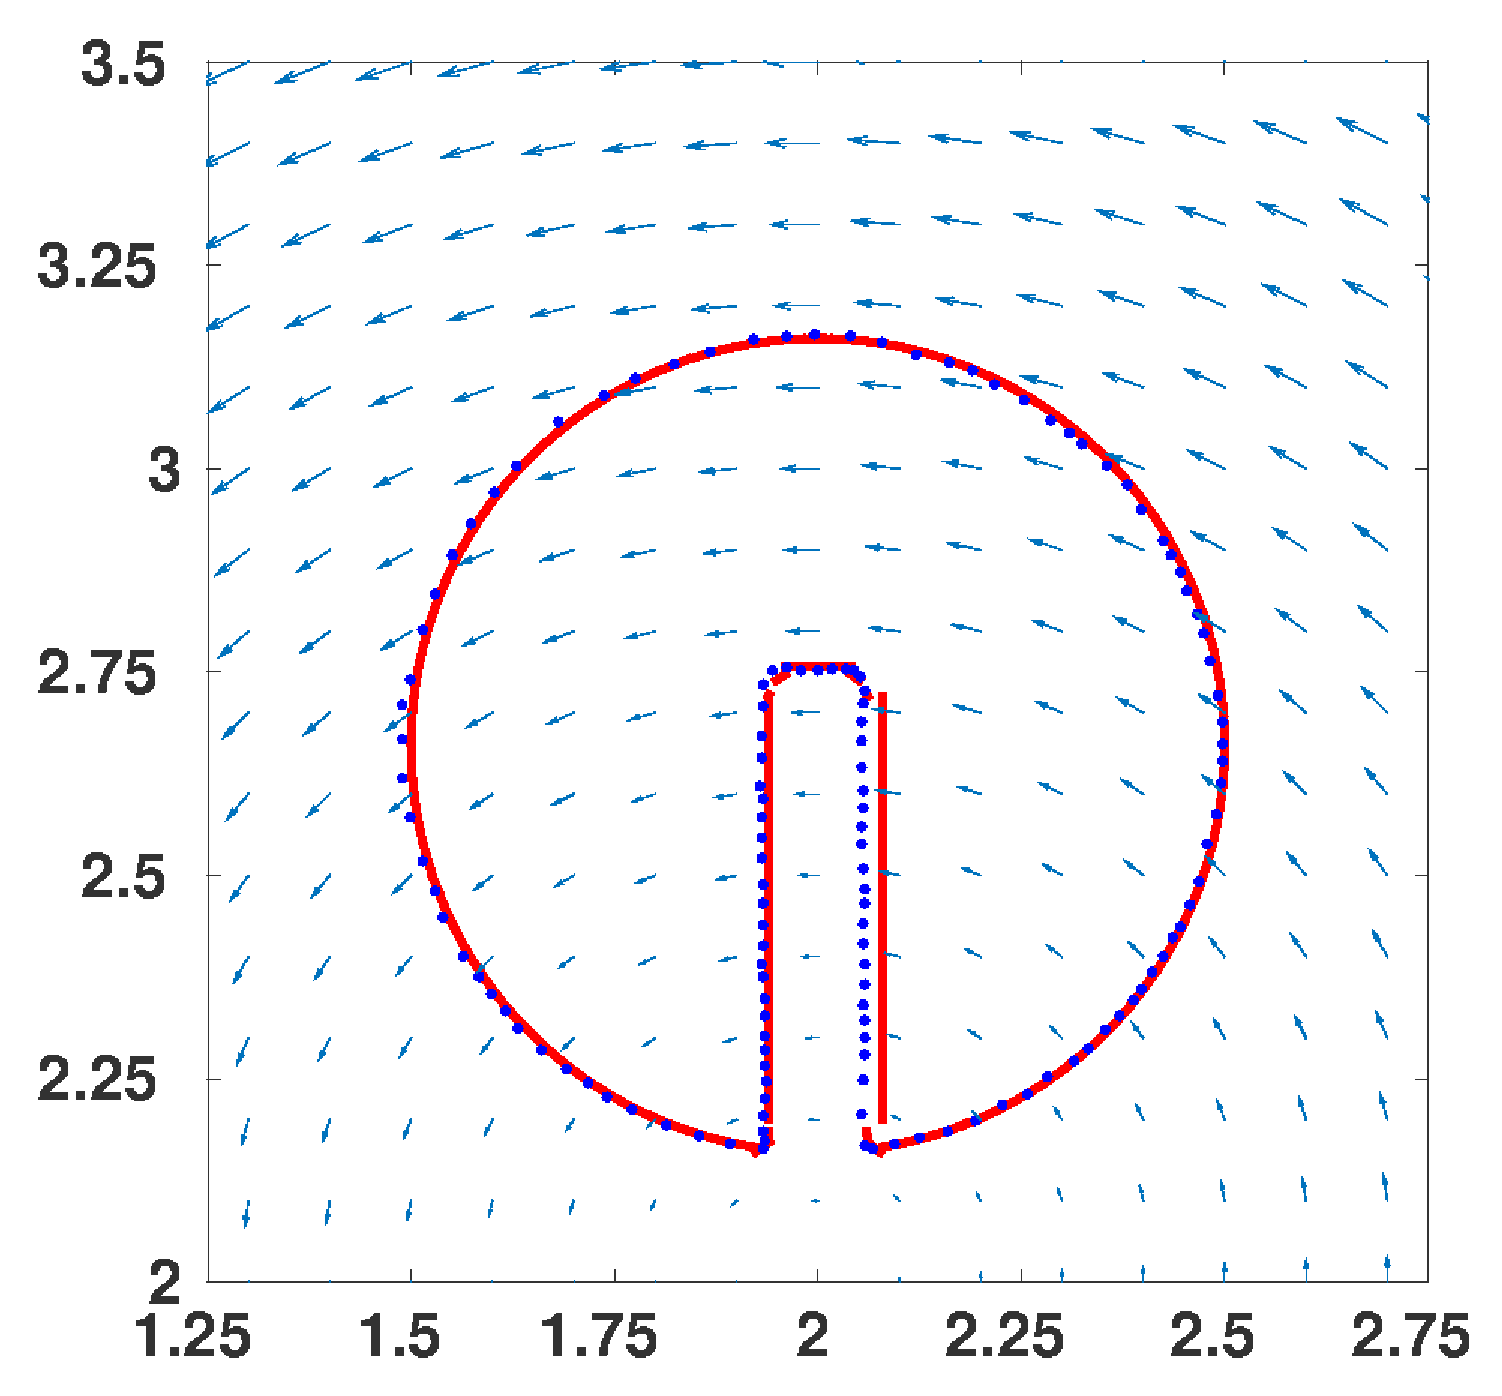
\includegraphics[width=0.5\textwidth]{SC_IC.eps}
      } 
  \subfloat[After one full rotation ]{%
      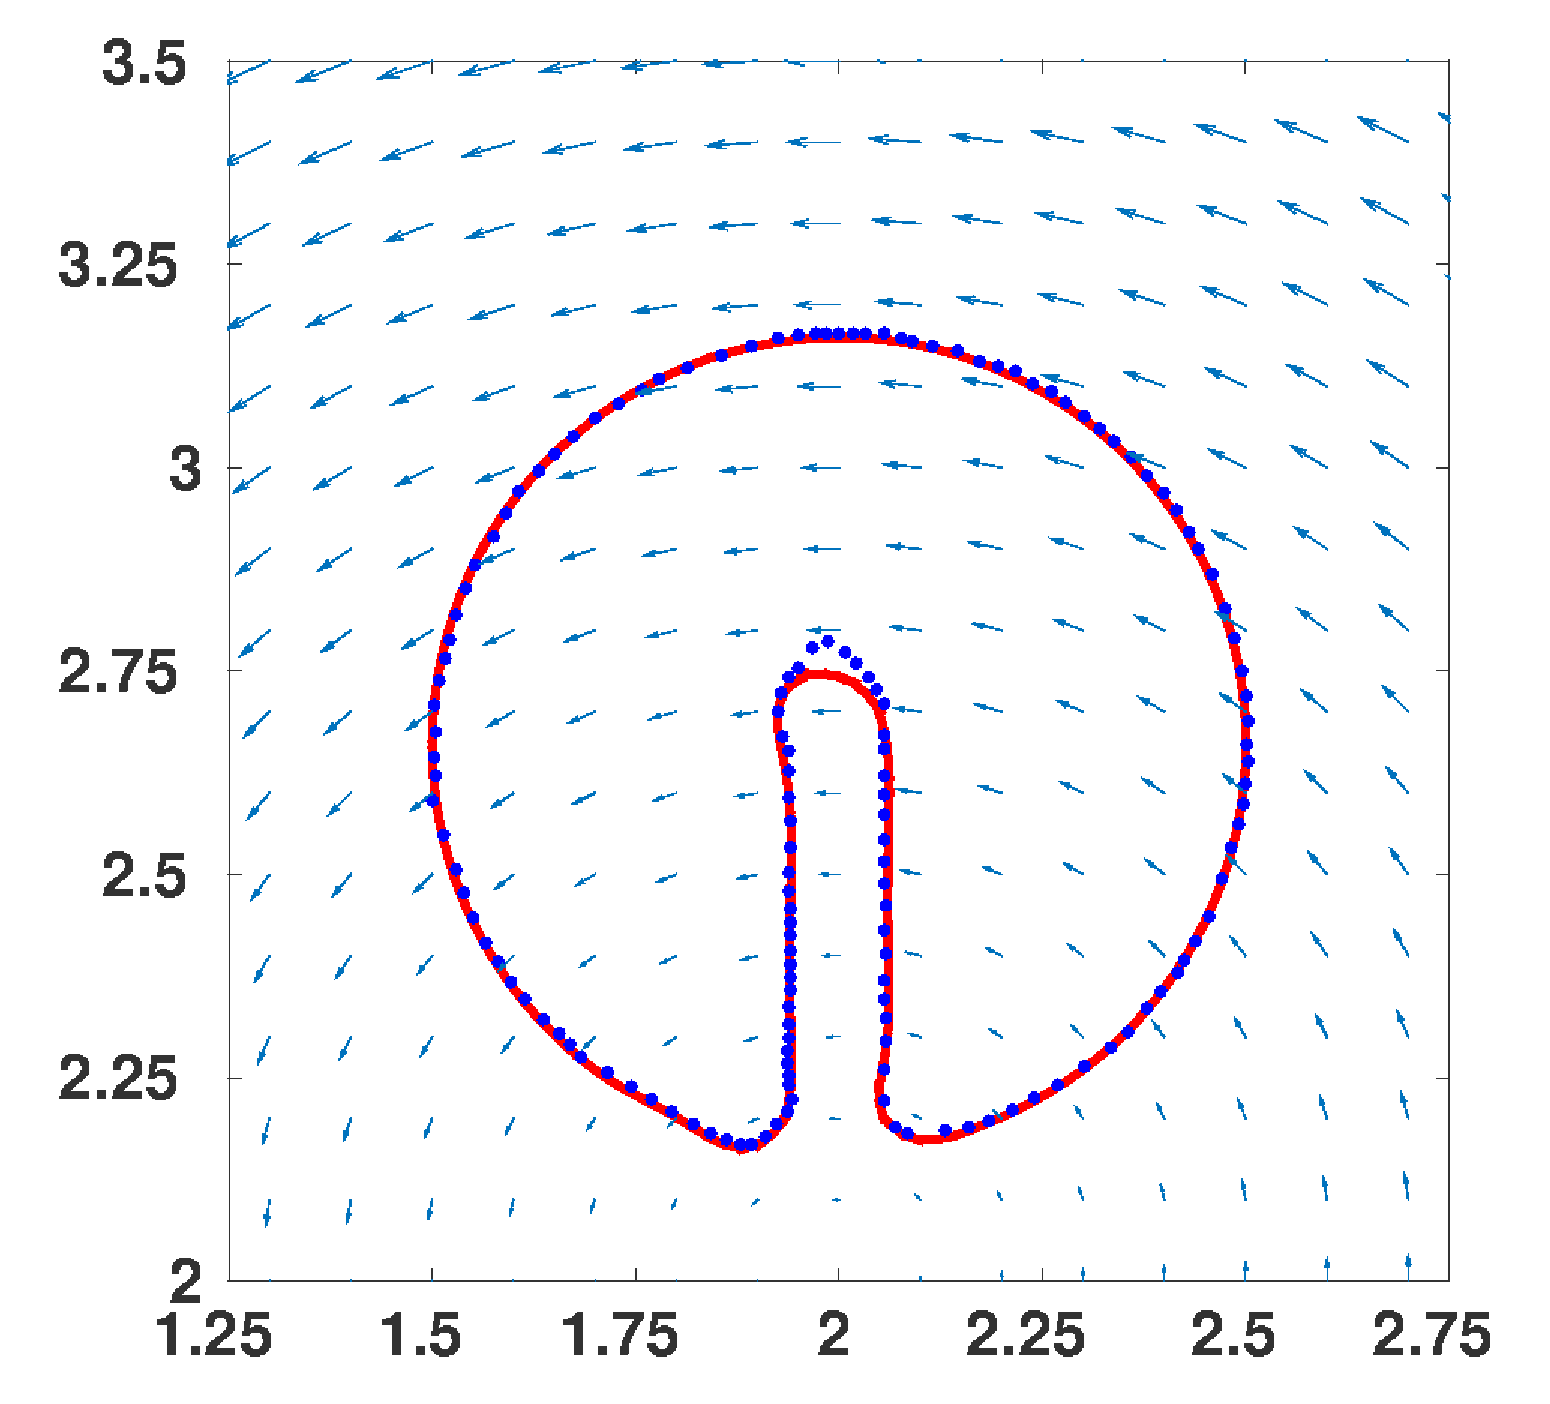
\includegraphics[width=0.5\textwidth]{SC_2513O.eps}
      }
 \caption{Comparison with \cite{Rudman1997} results. (Red LVIRA and Blue \cite{Rudman1997} data)}
 \label{Fig:rotation}
\end{figure}

\subsection{Shear Test}
The real problems typically encounters the interface deformation, which includes merging and deformation. Hence the algorithm has to be 
tested for shear velocity field (Figure \ref{Fig:shear}). The shear test problem verified with \cite{Gerlach2006}. (Figure \ref{Fig:shear_comparison}) 

   \begin{enumerate}
 \item Domain: [0,$\pi$] x [0,$\pi$]
 \item Grid Size: 100 x 100
 \item Radius of circle :$\frac{\pi}{5}$
 \item Center : $(\pi/2,\pi/4)$
 \item Velocity field(Forward):  $u=sin x cos y, v=-cos x sin y$
  \item Velocity field(Backward):  $u=-sin x cos y,v=cos x sin y$
 \end{enumerate}
 
\begin{figure}
\centering
   \subfloat[Initial condition for shear test ]{%
      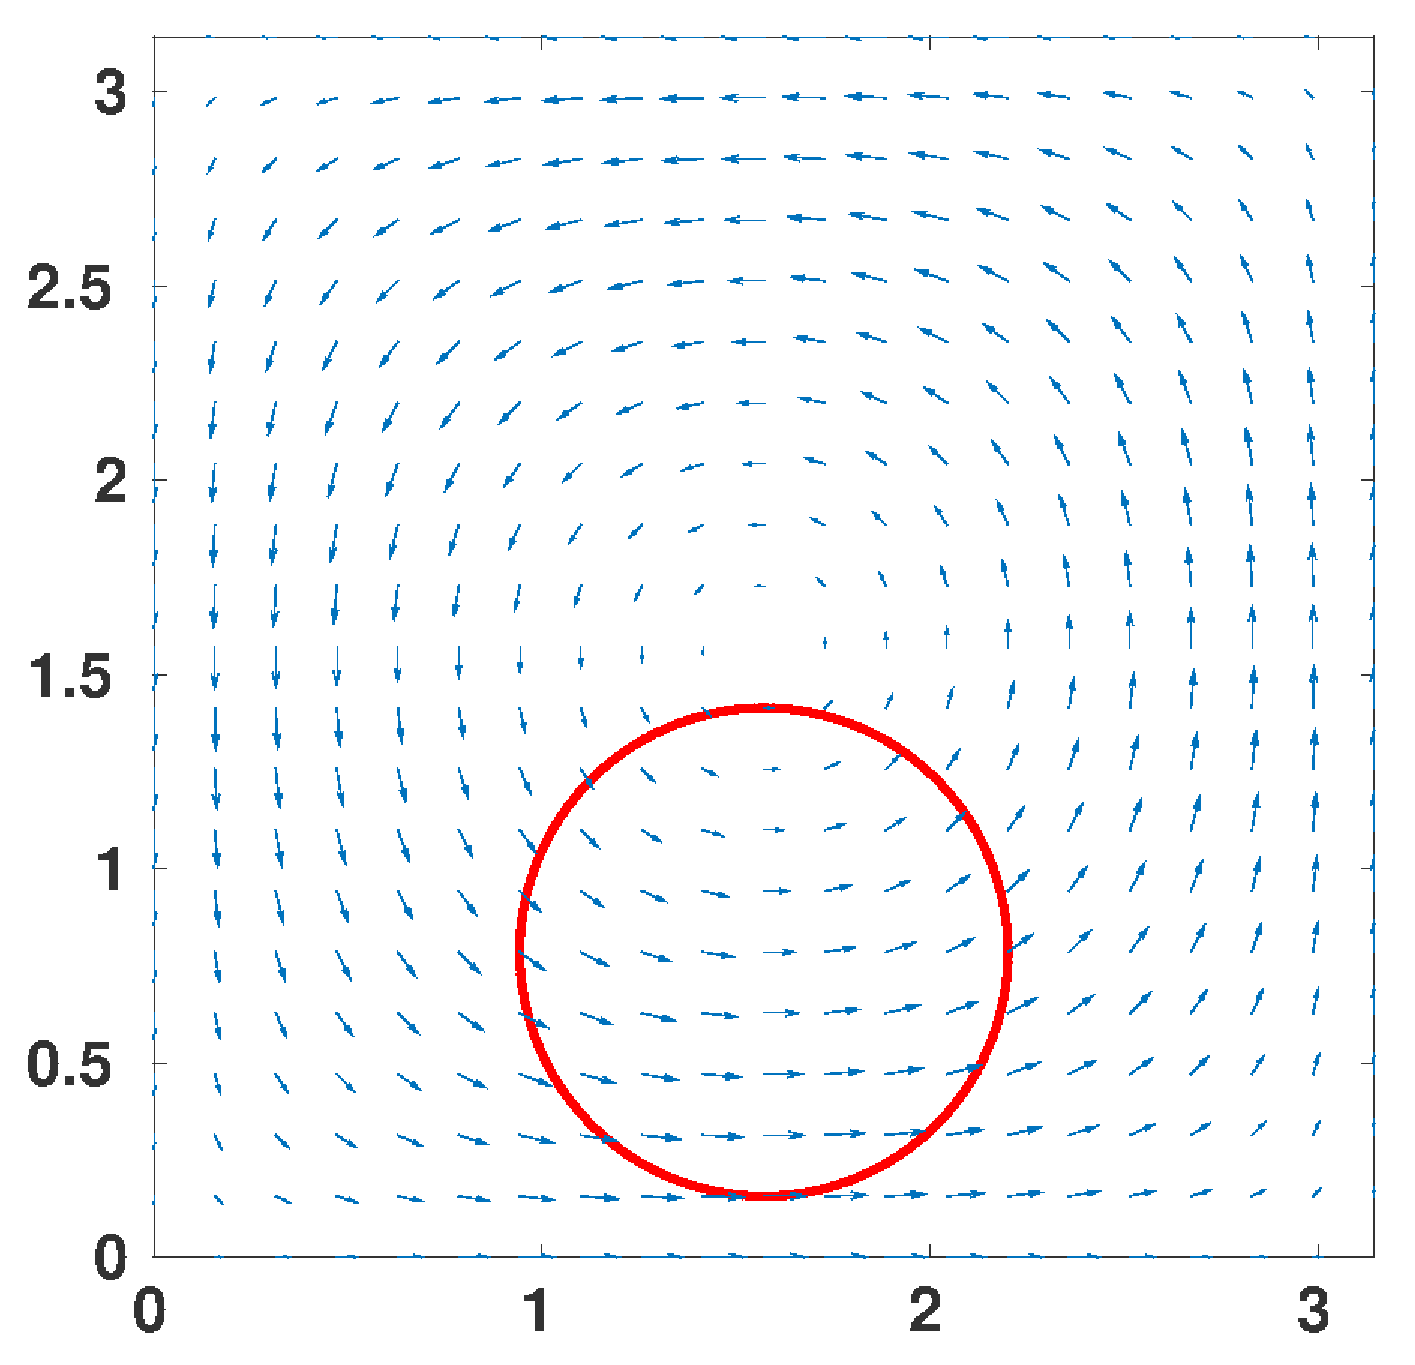
\includegraphics[width=0.5\textwidth]{shear_IC.eps}
      }
\subfloat[After advecting 250 steps ]{%
      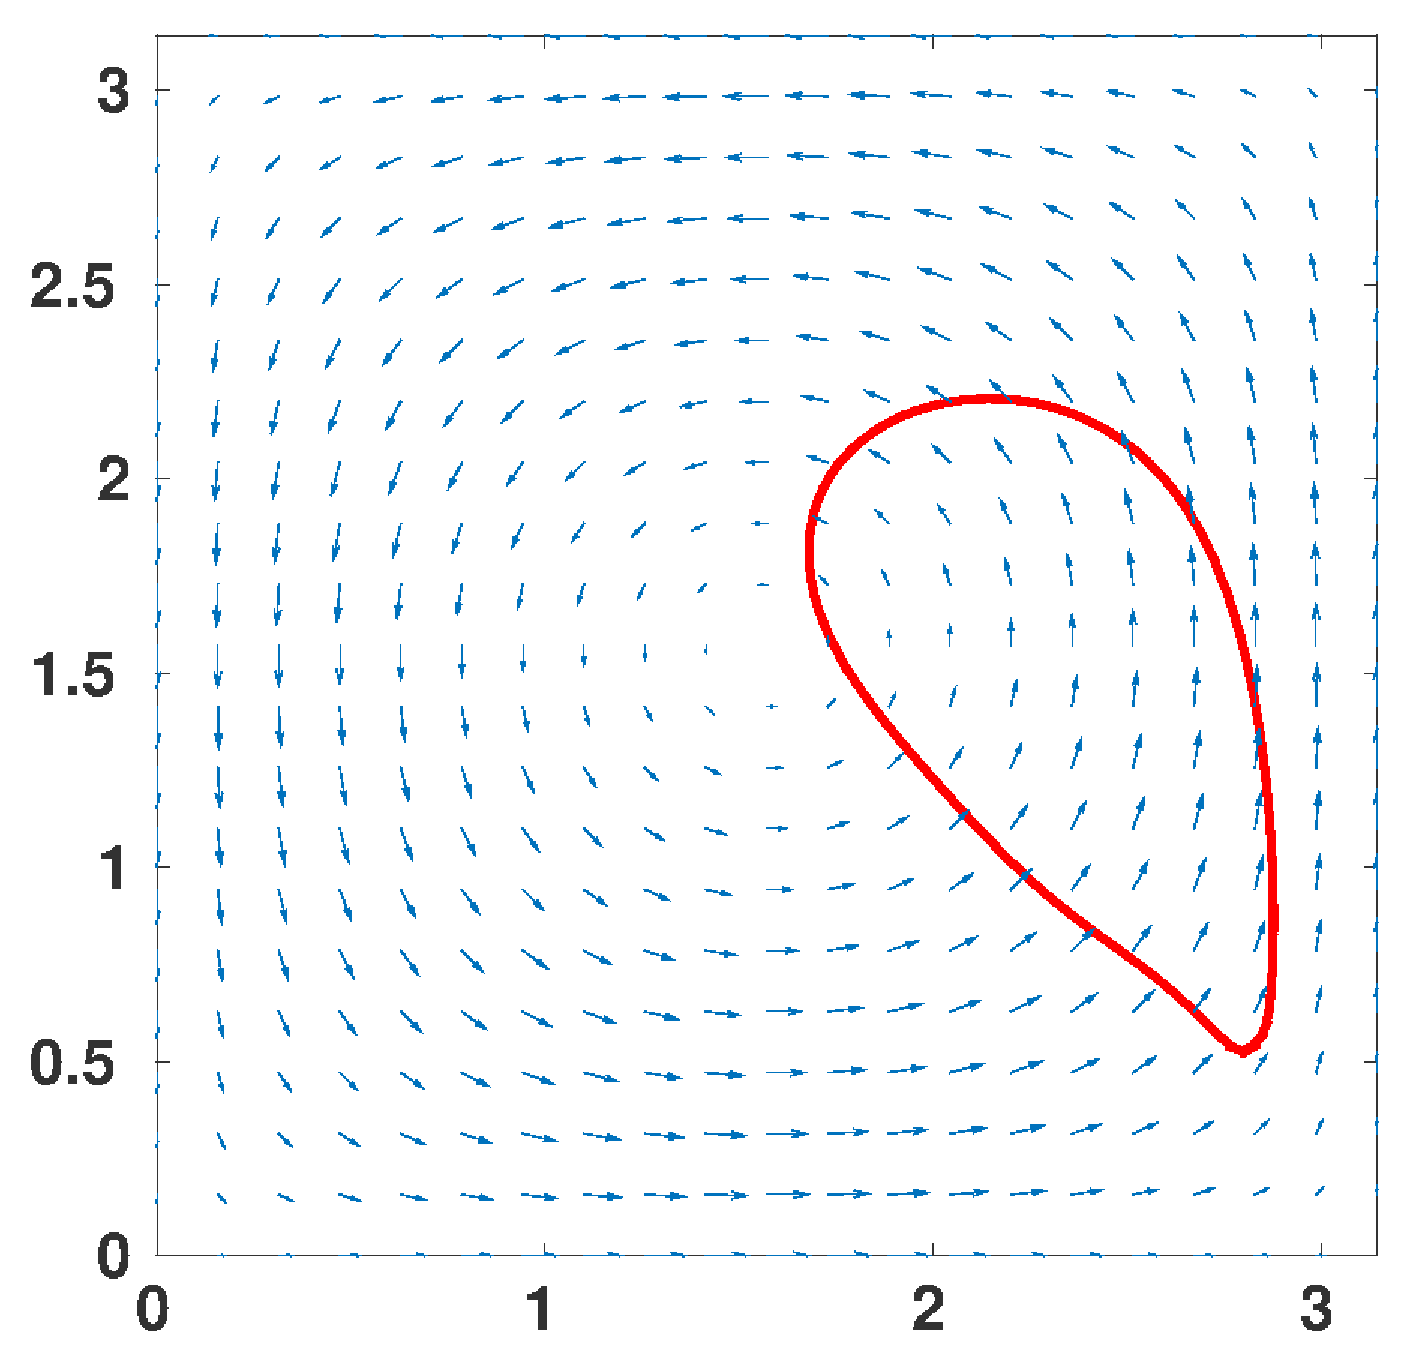
\includegraphics[width=0.5\textwidth]{shear_250.eps}
      } \\
      \subfloat[After advecting 500 steps ]{%
      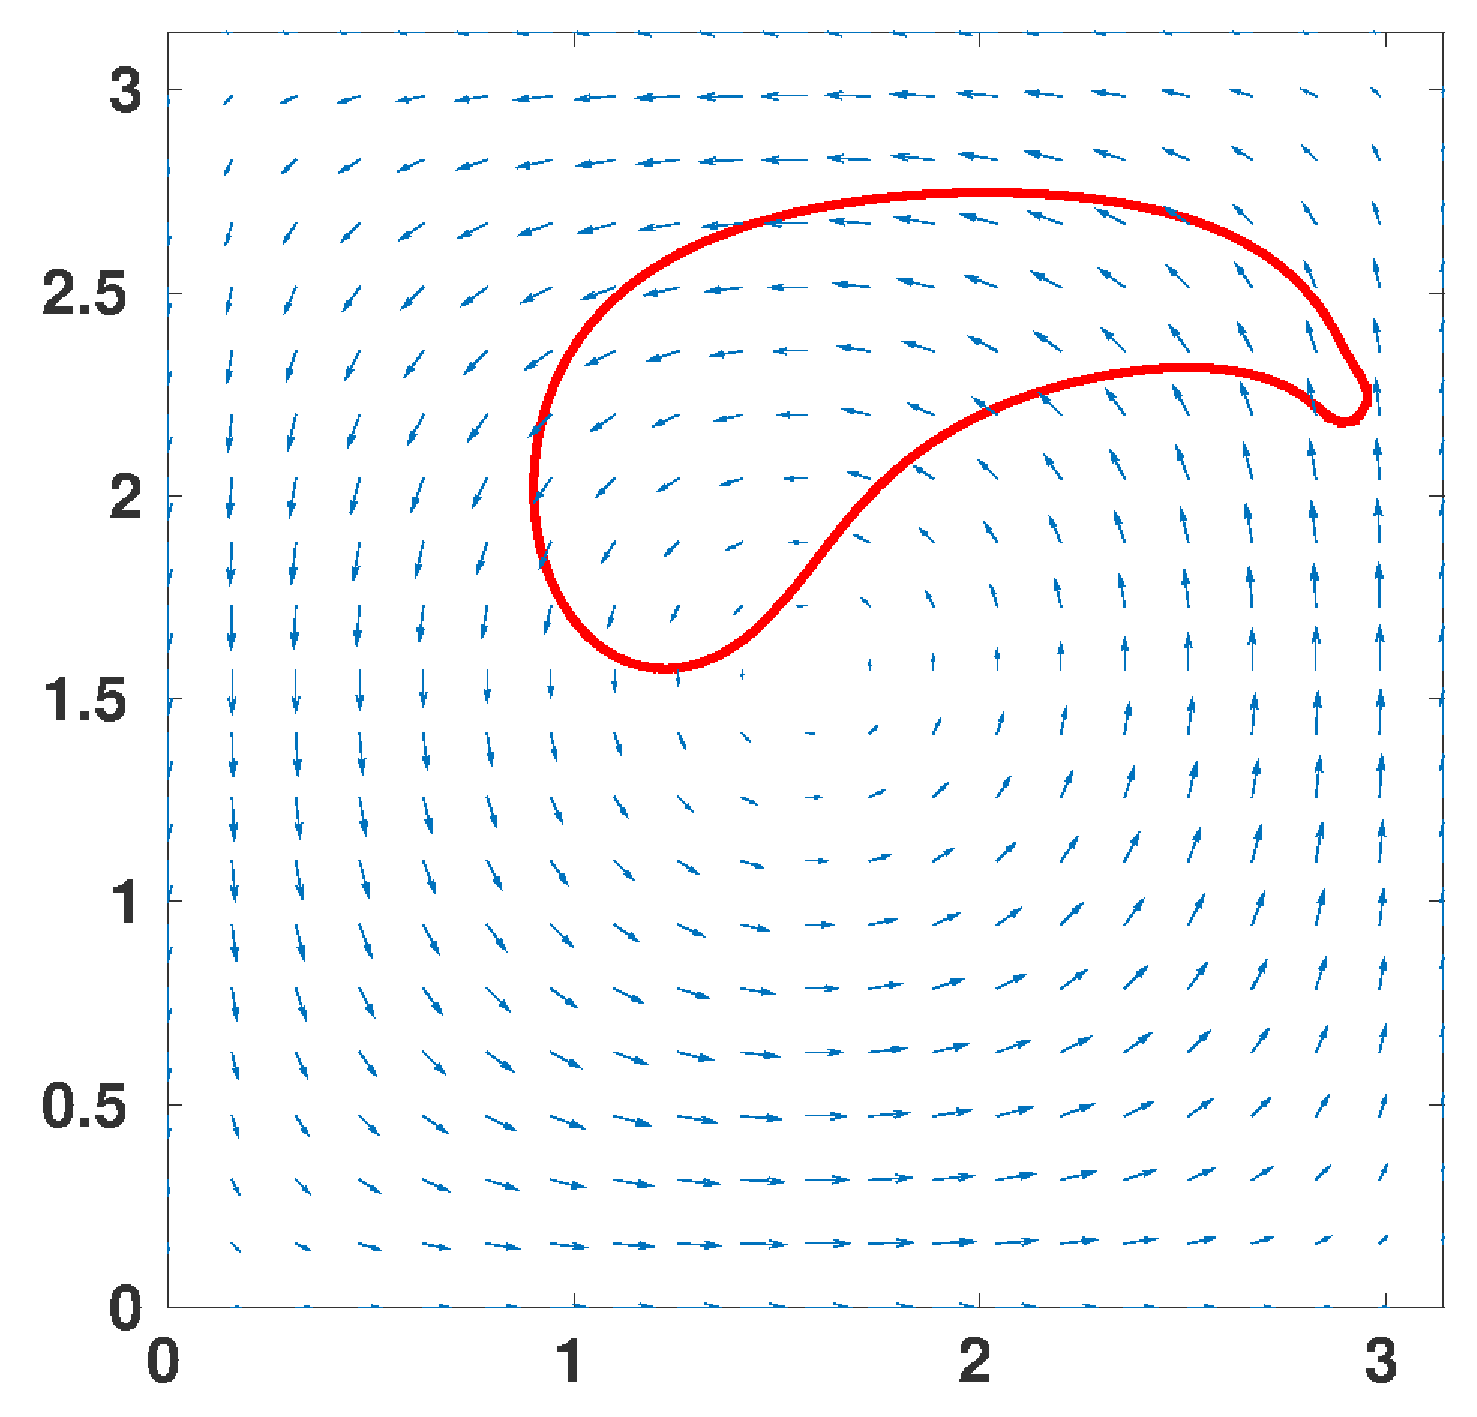
\includegraphics[width=0.5\textwidth]{shear_500.eps}
      }
      \subfloat[After advecting 1000 steps ]{%
      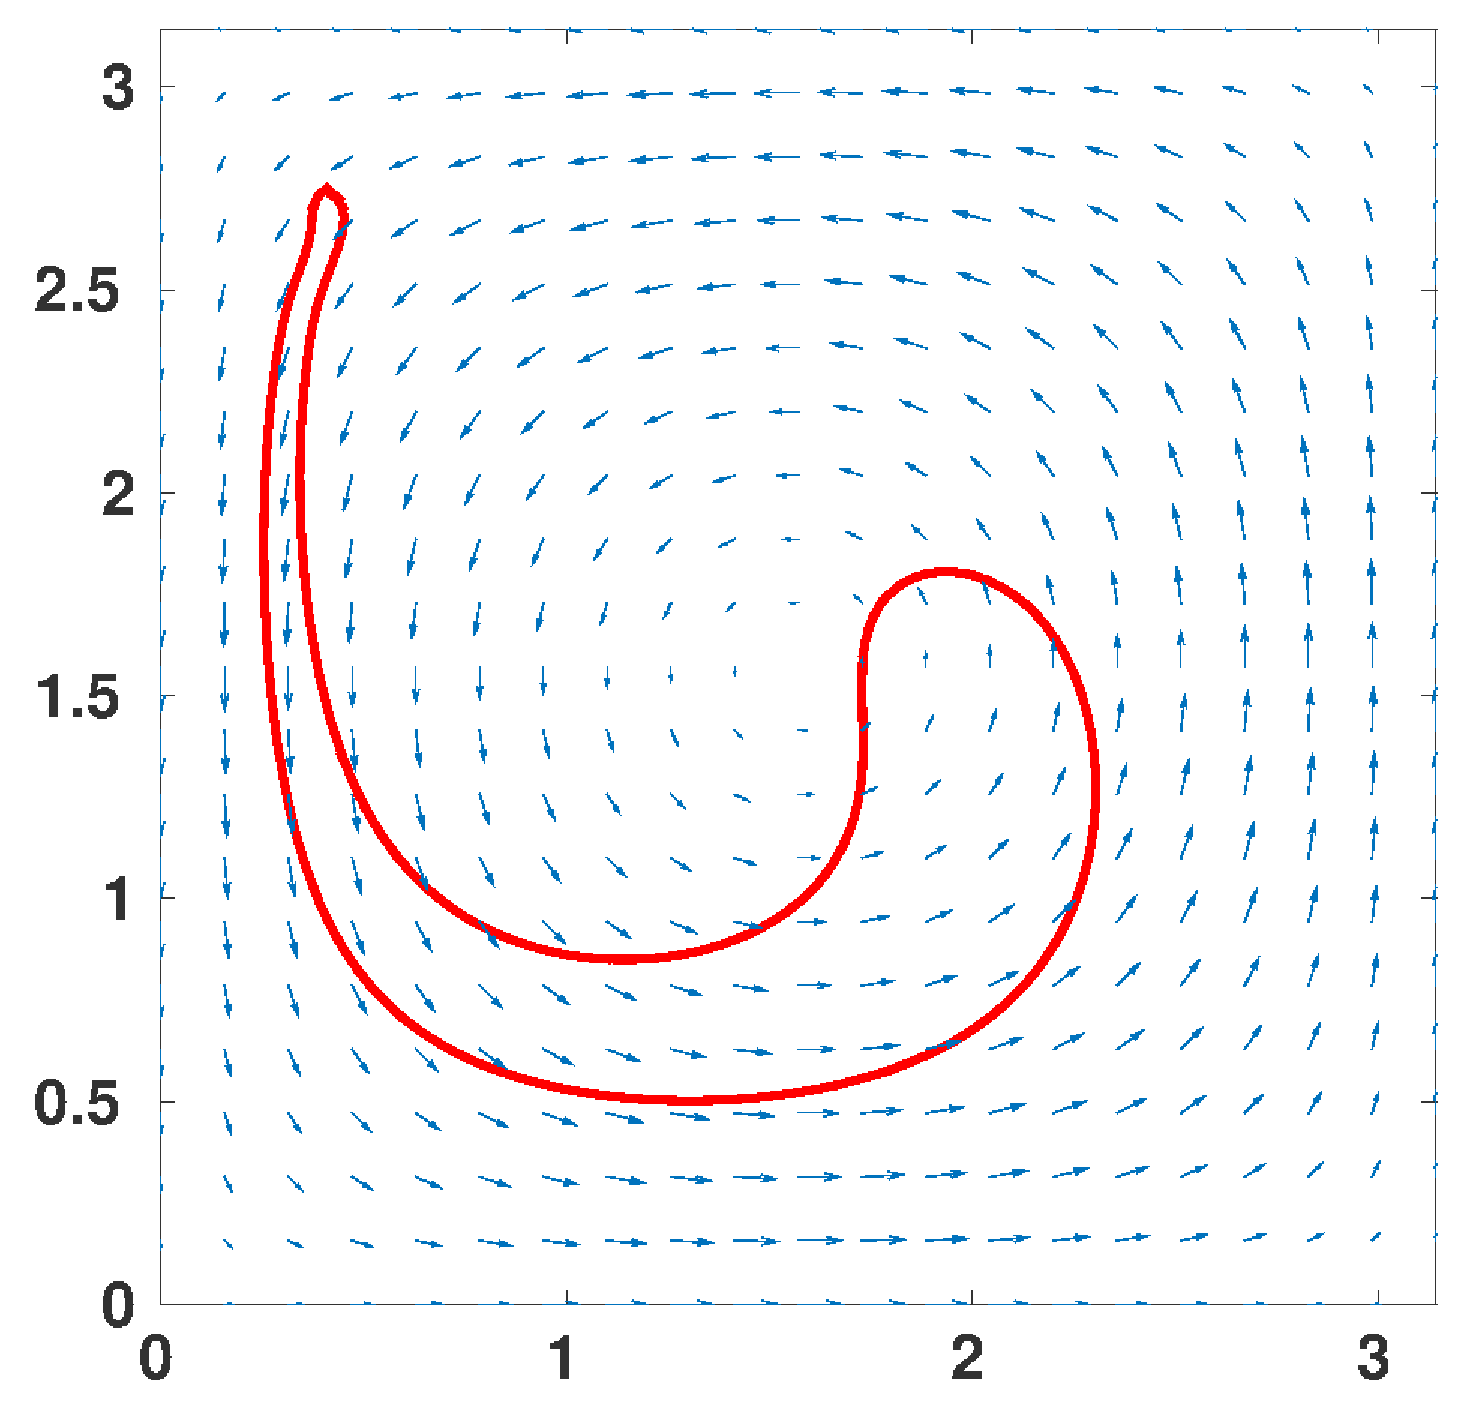
\includegraphics[width=0.5\textwidth]{shear_1000.eps}
      }
 \caption{Advection test result for shear velocity field}
 \label{Fig:shear}
\end{figure}

\begin{figure}
 \centering
 \subfloat[After 1000 steps forward ]{%
      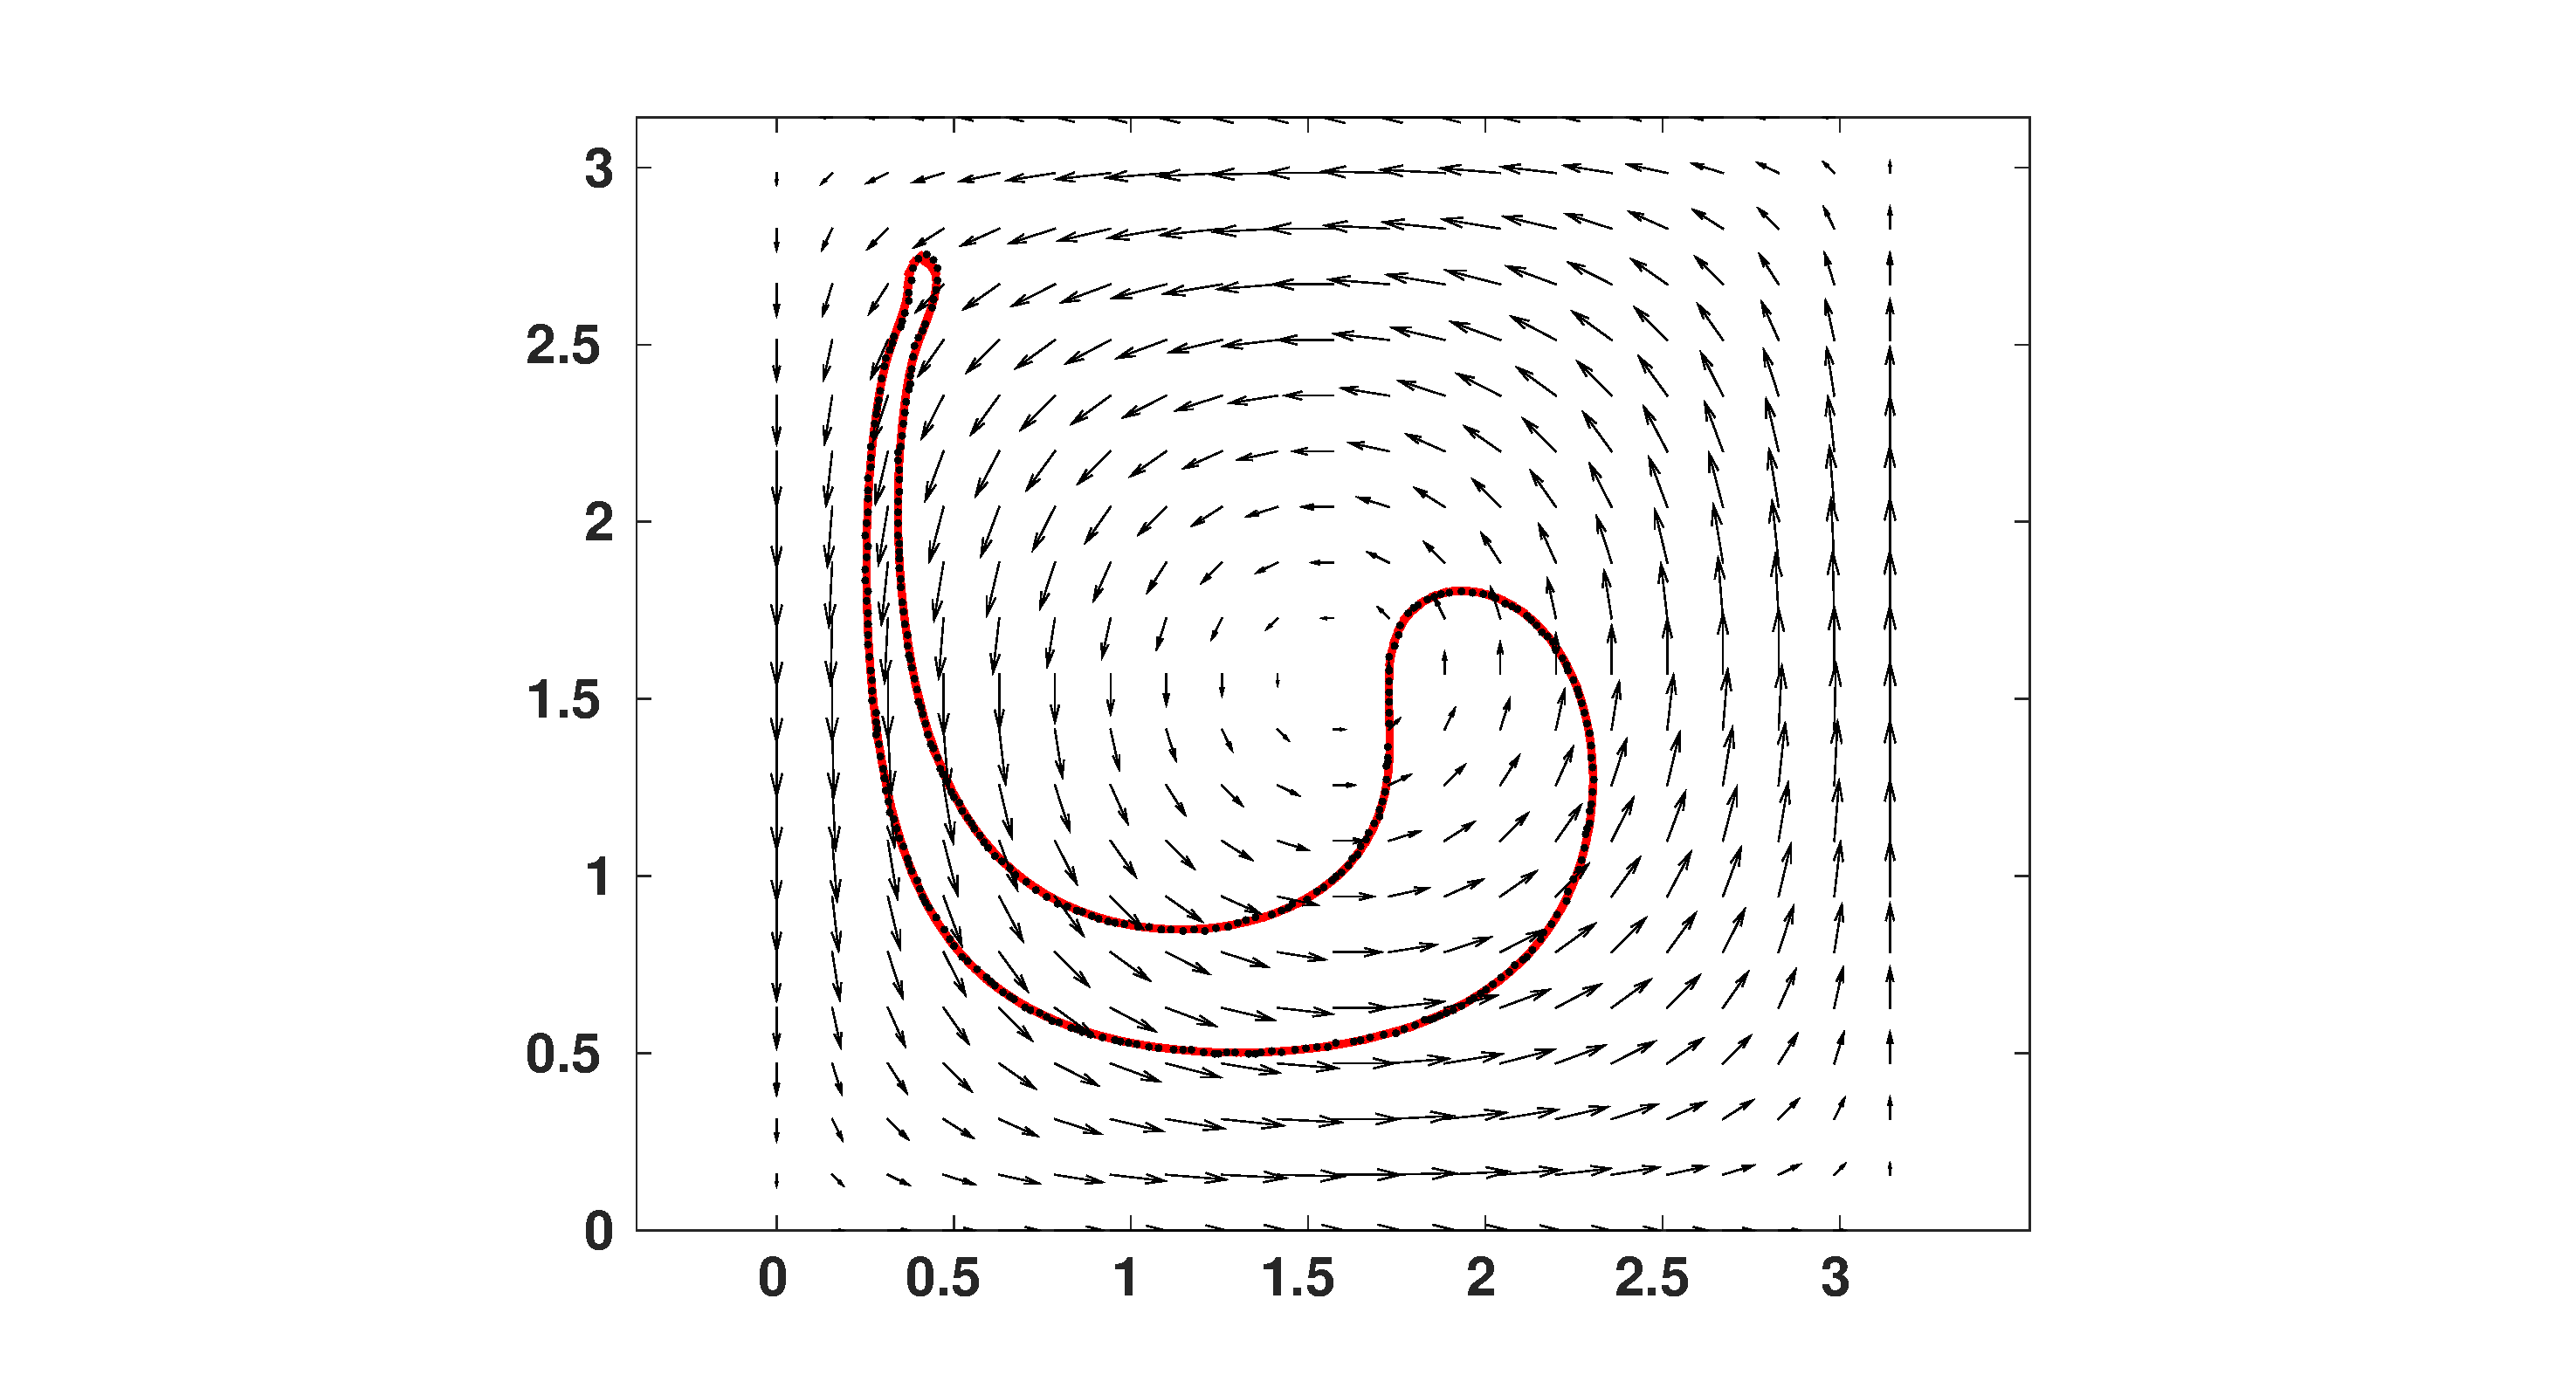
\includegraphics[width=0.5\textwidth]{shear_1000c.eps}
      }
  \subfloat[1000 steps backward followed by 1000 steps forward ]{%
      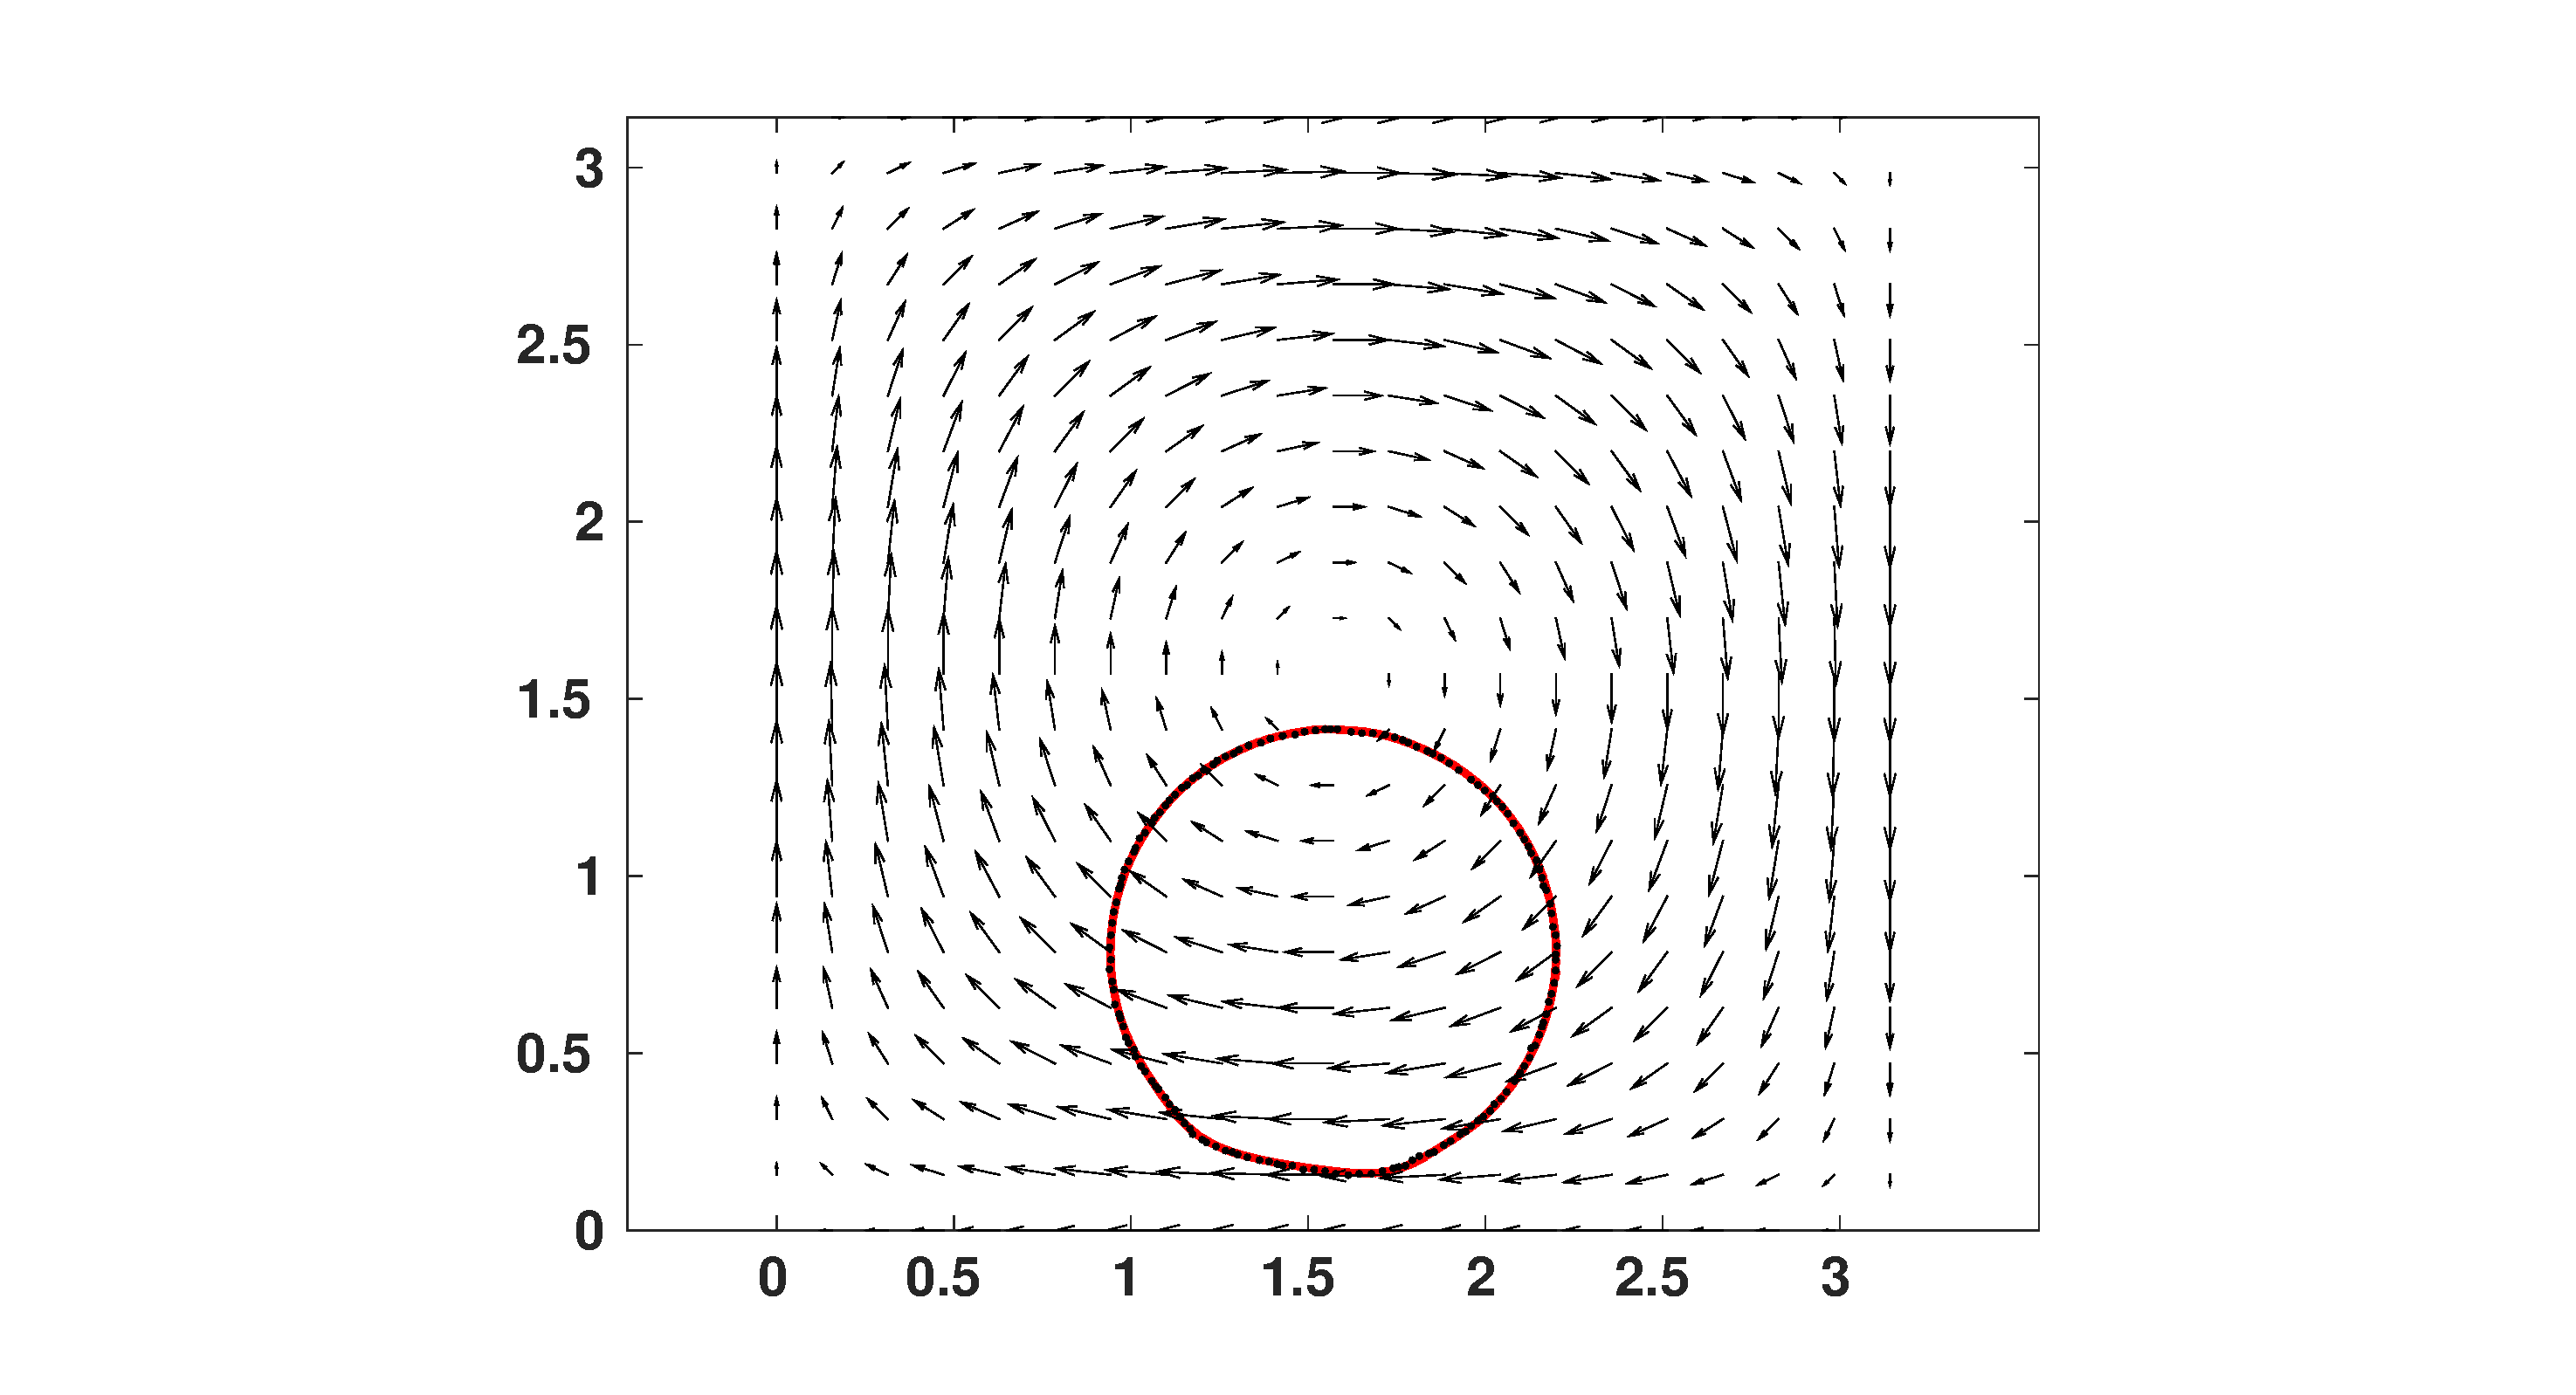
\includegraphics[width=0.5\textwidth]{shear_back.eps}
      }
 \caption{Comparison with \cite{Gerlach2006} results. (Red LVIRA and Blue \cite{Gerlach2006} data)}
 \label{Fig:shear_comparison}
\end{figure}

\subsection{Calculation of error}

The above results can be quantified by defining the error as
\begin{equation}
 E = \frac{\sum |{F^n_{r,c}-F^e_{r,c}}|}{\sum F^0_{r,c}}
\end{equation}
where E is the ratio of summation of difference between the volume fraction of cells of calculated solution and exact solution to the total sum inital volume fraction over all the cells.
where $F^n$ is the solution of volume fraction field after n time steps of computation, $F^e$ is the exact solution, and $F^0$ is the initial solution. The initial solution can be calculated by the initial 
volume fraction field, exact solution of field for translational velocity fields can be easily calculated by recreating the circle at the center which has moved with the velocity field. For solid body
rotation the exact solution is equal to the initial solution after one full rotation. For the shear test after 1000 backward steps the final solution should also be equal to initial solution.
The errors calculated for various tests are shown in Table \ref{Table:errors} and compared with \cite{Rudman1997}.

\begin{table}
  \begin{center}
    \caption{Errors for various tests}
 \label{Table:errors}
    \begin{tabular}{p{3cm}llll|a}
      \toprule 
       Test & SLIC & Hirt-Nichols & FCT-VOF & Youngs & LVIRA (Present Study)  \\ 
      \midrule
      Translational (V(1,0)) & $1.30 X 10^{-2}$ & $4.55 X 10^{-2}$ & $1.28 X 10^{-2}$ & $3.08 X 10^{-3}$ & $1.5 X 10^{-3}$  \\ 
        Translational (V(2,1)) & $9.18 X 10^{-2}$ & $1.9 X 10^{-1}$ & $3.99 X 10^{-2}$ & $2.98 X 10^{-2}$ & $1.05 X 10^{-2}$  \\ 
      Shear Flow & $4.59 X 10^{-2}$ & $6.66 X 10^{-2}$ & $3.14 X 10^{-2}$ & $8.60 X 10^{-3}$ & $6.90 X 10^{-3}$  \\ 
       Solid Body Rotation (Slotted circle) & $8.38 X 10^{-2}$ & $9.62 X 10^{-2}$ & $3.29 X 10^{-2}$ & $1.09 X 10^{-2}$ & $9.7 X 10^{-3}$  \\ 
        
      \bottomrule \\
    \end{tabular}
  \end{center}
\end{table}


\section{Conclusion}
The reconstruction and advection of an interface is calculated mostly geometrical techniques and does not require extensive knowledge of computational techniques. We found LVIRA
is more accurate than other methods available in the literature. We will couple this algorithm with a flow solver which we have discussed in the next chapter. 